%---------
% PREAMBLE
%---------
\documentclass[aspectratio=169, xcolor=dvipsnames]{beamer} % Set aspect-ratio and add color classes (svgnames, dvipsnames)

% PACKAGES
\usepackage{hyperref} % Allows including hyperlinks
\usepackage{graphicx} % Allows including images
\usepackage{csquotes} % Allows the use of quotations
\usepackage{xcolor}
\usepackage{subcaption} % Allows for side-by-side images
\usepackage{arydshln} 
\usepackage{comment} % Commenting out multiple lines
\usepackage{lmodern}
\usepackage[T1]{fontenc}
\usepackage{bm,graphics}
\usepackage{longtable}
\usepackage{beamerthemesplit}
\usepackage{makeidx,epsfig,lscape}
\usepackage{amsmath}
\usepackage{amssymb}
\usepackage{listings}
\usepackage{accents}

% PACKAGES | TIKZ
\usepackage{tikz}
\usetikzlibrary{decorations.pathreplacing,calc, fit}

% PACKAGES | TABLES
\usepackage{multirow}
\usepackage{booktabs} % Allows the use of \toprule, \midrule and \bottomrule in tables
\usepackage{tabularx}

% MATH
\newcommand{\ceil}[1]{\left\lceil #1 \right\rceil}

% BIBLIOGRAPHY
\usepackage[style=apa,sortcites=true,sorting=nyt,backend=biber]{biblatex}
\addbibresource{references.bib}
\AtBeginBibliography{\small} % Change reference font size to small

% HANDOUTS
\usepackage{pgfpages}
%\pgfpagesuselayout{2 on 1}[a4paper,border shrink=5mm]

% THEME
\usetheme{Warsaw}
\useinnertheme{rounded,circles} % Inner themes: default,circles,inmargins,rectangles,rounded

% COLOR
\definecolor{ashgrey}{rgb}{0.68, 0.75, 0.71}
\definecolor{ashgreyl}{rgb}{.96,.98,.98}
\definecolor{charcoal}{rgb}{0.21, 0.27, 0.31}
\definecolor{MyRed}{rgb}{0.93, 0.35, 0.35}
\definecolor{gray60}{rgb}{0.6, 0.6, 0.6}
\definecolor{gray20}{rgb}{0.2, 0.2, 0.2}

\usecolortheme{seagull} %innercolorthemes:seahorse,orchid,lily,rose,seagull,albatross,beetle,crane,dove,fly,whale

\setbeamercolor{frametitle}{bg=ashgrey, fg=black}
\setbeamercolor{title}{bg=ashgrey}
\setbeamercolor{itemize item}{fg=black}
\setbeamercolor{block title}{bg=ashgrey}
\setbeamercolor{block body}{bg=ashgreyl}
\setbeamercolor{example text}{fg=NavyBlue}
\setbeamercolor{umbcboxes}{bg=green!15,fg=black}
\setbeamercolor{example text}{fg=NavyBlue}
\setbeamercolor{umbcboxes}{bg=green!15,fg=black}

% FONT
\usefonttheme[onlymath]{serif}

% R CODE
\lstset{
    language=R,
    commentstyle=\color{gray60},
    keywordstyle=\color{gray20},
    numberstyle=\ttfamily\footnotesize\color{gray60},
    stringstyle=\color{black},
    basicstyle=\ttfamily\small,
    breakatwhitespace=false,         
    breaklines=true,                 
    captionpos=b,                    
    keepspaces=true,                 
    numbers=left,                    
    numbersep=5pt,                  
    showspaces=false,                
    showstringspaces=false,
    showtabs=false,                  
    tabsize=2,
    morekeywords={\%*\%}
}

% TEMPLATE
\setbeamertemplate{frametitle}[default][left]
\setbeamertemplate{headline}{} % Get rid of upper navigation menu
\setbeamertemplate{navigation symbols}{} % Get rid of navigation symbols 
\setbeamertemplate{footline}[frame number] % Use frame number rather than page number

\AtBeginSection[]{
    \begin{frame}
        \frametitle{Table of contents}
        \tableofcontents[currentsection]
    \end{frame}
}

\AtBeginSubsection[]{
  \begin{frame}
      \vfill
      \centering
      \begin{beamercolorbox}[sep=8pt,center,shadow=true,rounded=true]{title}
        \usebeamerfont{title}\insertsubsectionhead\par%
      \end{beamercolorbox}
      \vfill
  \end{frame}
}


%-----------
% TITLE PAGE  
%-----------
\title[]{Time Aggregation and Missing Time Frames in Causal Research With Panel Data}
\author[]{Jeroen D. Mulder\inst{1}, Manuel C. Voelkle\inst{2}, Ellen L. Hamaker\inst{1}}
\institute[]{
    \inst{1} Universiteit Utrecht\\
    \inst{2} Humboldt-Universität
}
\date{Donnerstag 26. September, 2024}

%--------------------
% PRESENTATION SLIDES
%--------------------
\begin{document}

\begin{frame}
    \titlepage % Print title page as first slide
\end{frame}

%---------------------
\section{Introduction}
%---------------------

\begin{frame}{Empirical example: Timing of measurements in LISS}
    Longitudinal Internet studies for the Social Sciences (LISS) panel gather \textbf{yearly} data of Dutch population on constructs such as \textit{physical activity} (average last week), \textit{mental health indicators} (average last month), \textit{self-esteem} (no measurement time-frame), etc.\\
    \bigskip
    \bigskip
    The analysis of such data typically involves:\\
    \bigskip
    \begin{itemize}
        \item Time-aggregation: ``How did you feel on average the last week/month?"\\
        \bigskip
        \item Missing time frames between discrete time time points. 
    \end{itemize}
\end{frame}

%-----------------------------------
\section{Single-Subject Analysis}
%-----------------------------------

%--------------------------------
\subsection{No Lagged Effects}
%--------------------------------

\begin{frame}{No lagged effects | \textcite{hickman_effects_1972}}
    Let capital letters refer to aggregated data, and small letters to disaggregated data. Further let the aggregation scheme for the \textbf{average} $R(L) = (1 + L + ... + L^{n - 1}) / n$, with $L$ the lag operator and $n$ the period of aggregation.\\
    \bigskip \pause
    Suppose we have the disaggregate model 
    \begin{equation} \label{eq:disaggregate-no-lagged}
        y_{t} = m x_{t} + u_{t}
    \end{equation}
    which we aggregate by applying $R(L)$ to both sides, giving
    \begin{equation} \label{eq:aggregate-no-lagged}
        Y_{t} = M X_{t} + U{t}. 
    \end{equation}
    \textcite{hickman_effects_1972} states that $m = M$, and that when $u_{t}$ is serially independent, then $U_{t}$ will also be. 
\end{frame} 

%----

\begin{frame}{No lagged effects | Data generation}
    \textbf{Exposure $X$:}\\
    Continuous Time Markov Chain with transition probabilities $q_{01} = 0.3$ and $q_{10} = 0.3$.\\
    \bigskip
    \textbf{Outcome $Y$:}\\
    Continuous measure, given by Equation~\ref{eq:disaggregate-no-lagged}.\\
    \bigskip
    \textbf{Aggregation-scheme:}\\
    Taking the mean over $n$ periods, where $n \in \{2, 3, 4\}$, and ensuring proper (i.e., nonoverlapping) aggregates. 
\end{frame}

%----

\begin{frame}{No lagged effect | Data visualization ($n = 4$)}
    \begin{figure}
        \centering
        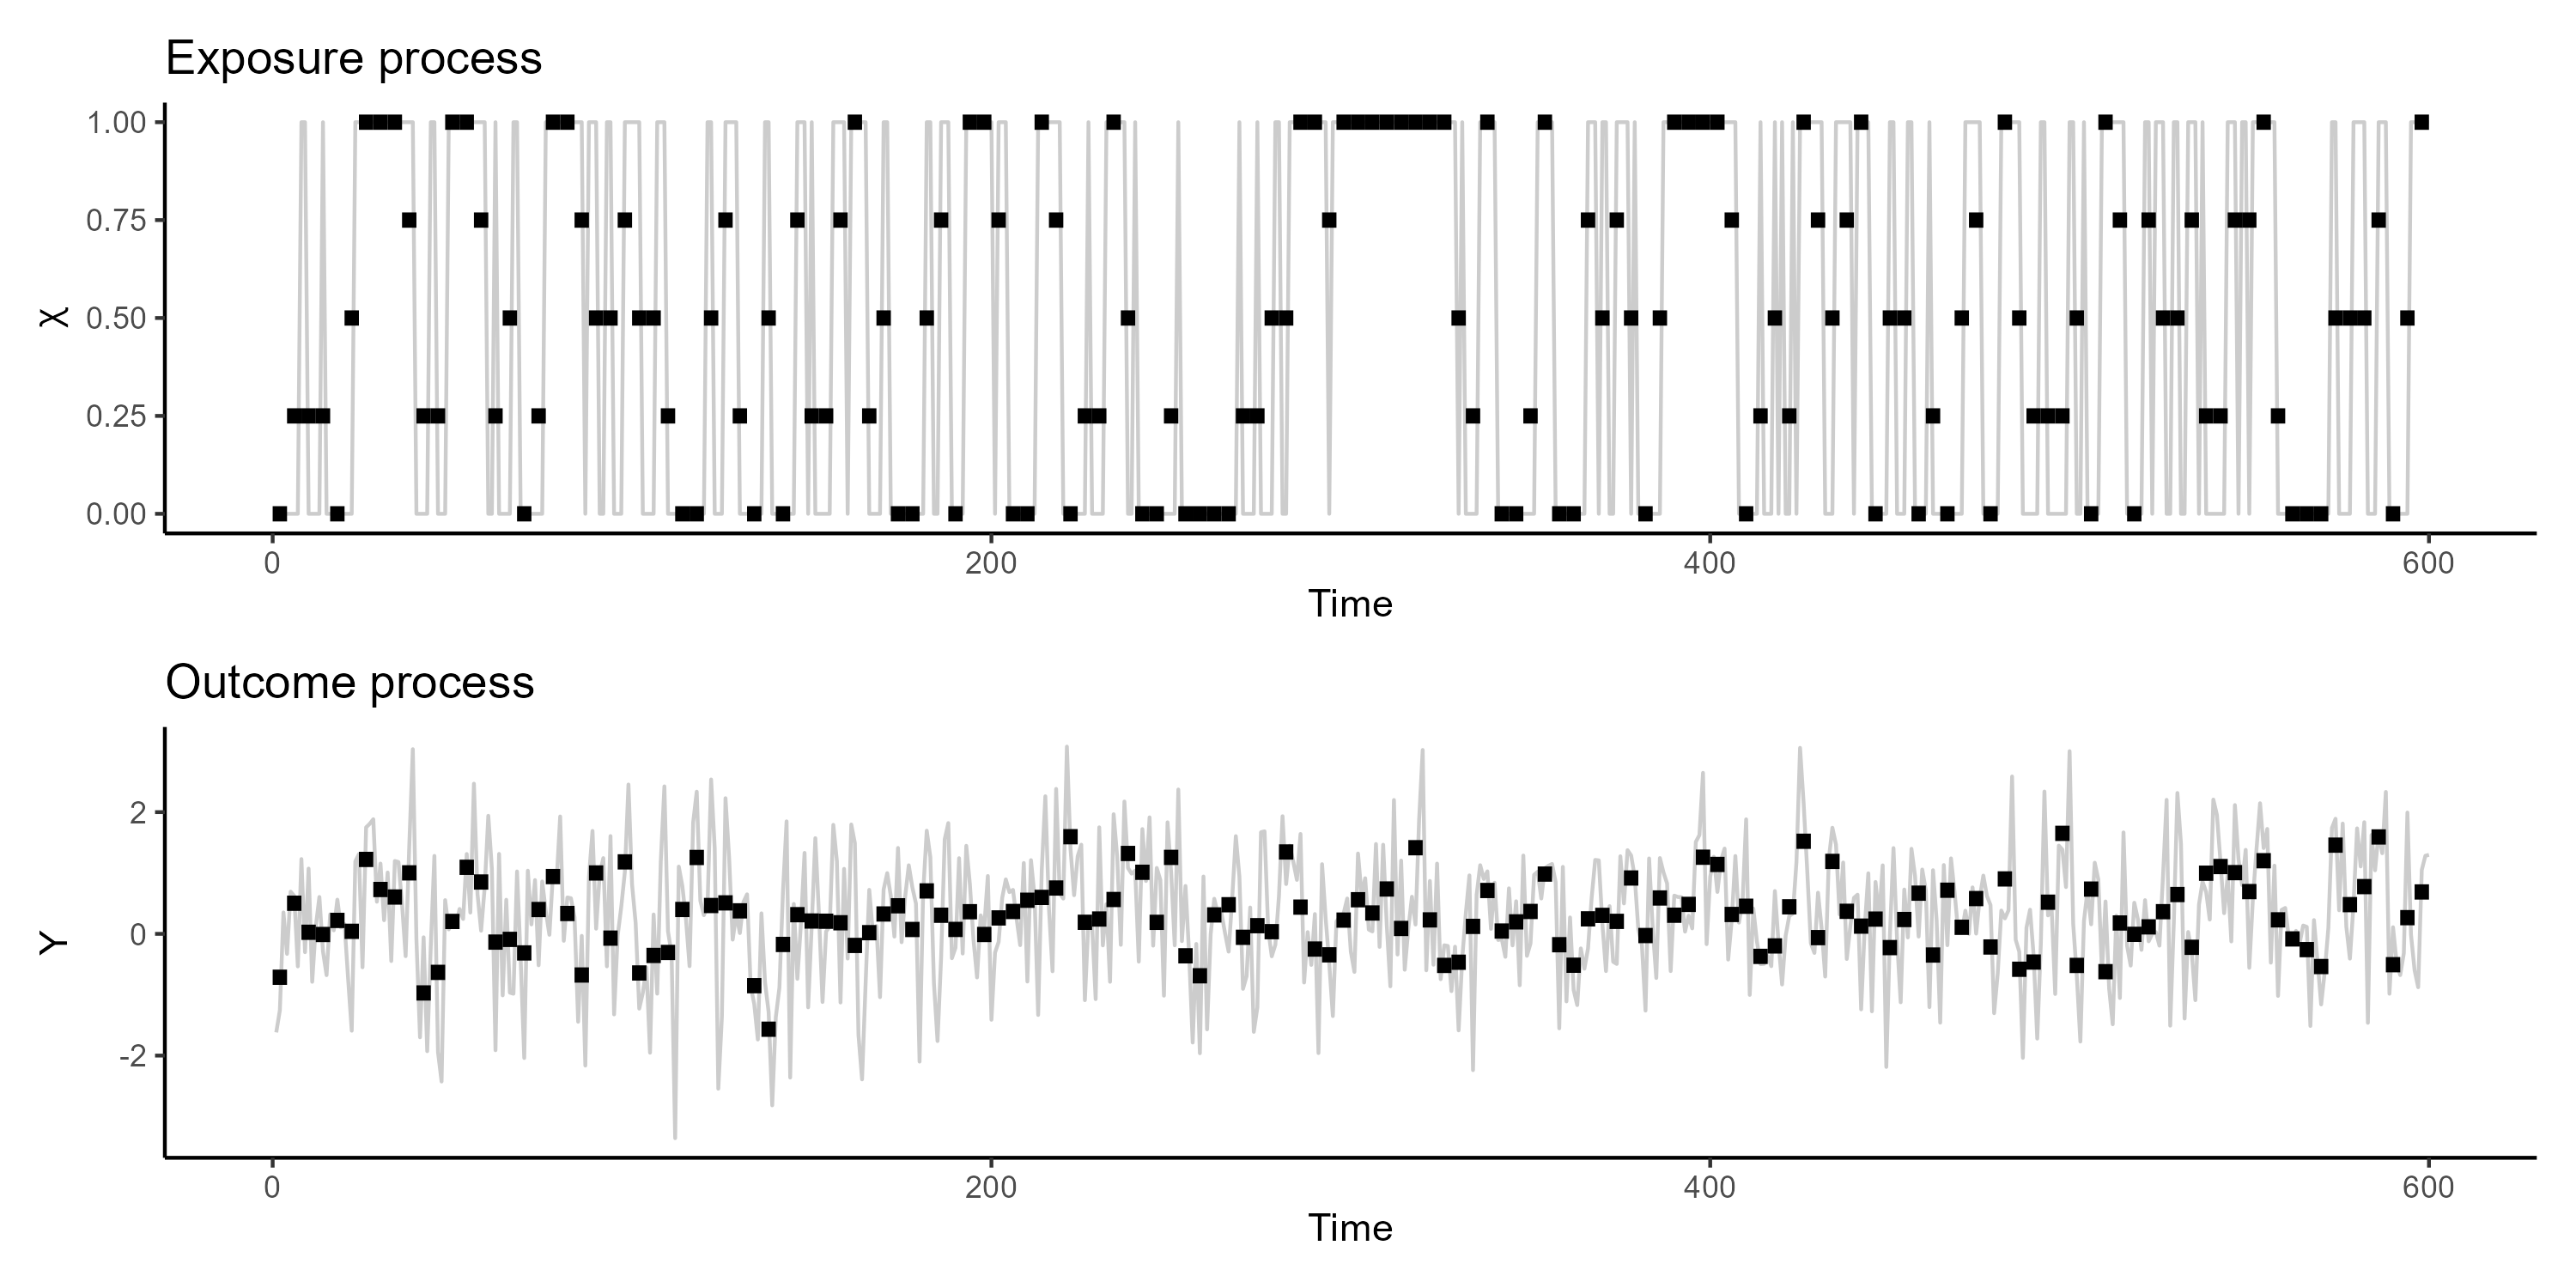
\includegraphics[width=1\textwidth]{figures/plot_singleSubject_noLag.png}
    \end{figure}
\end{frame}

%----

\begin{frame}{No lagged effects | Results (sampling distribution)}
    \begin{columns}
        \begin{column}{.5\textwidth}
            \begin{figure}
                \centering
                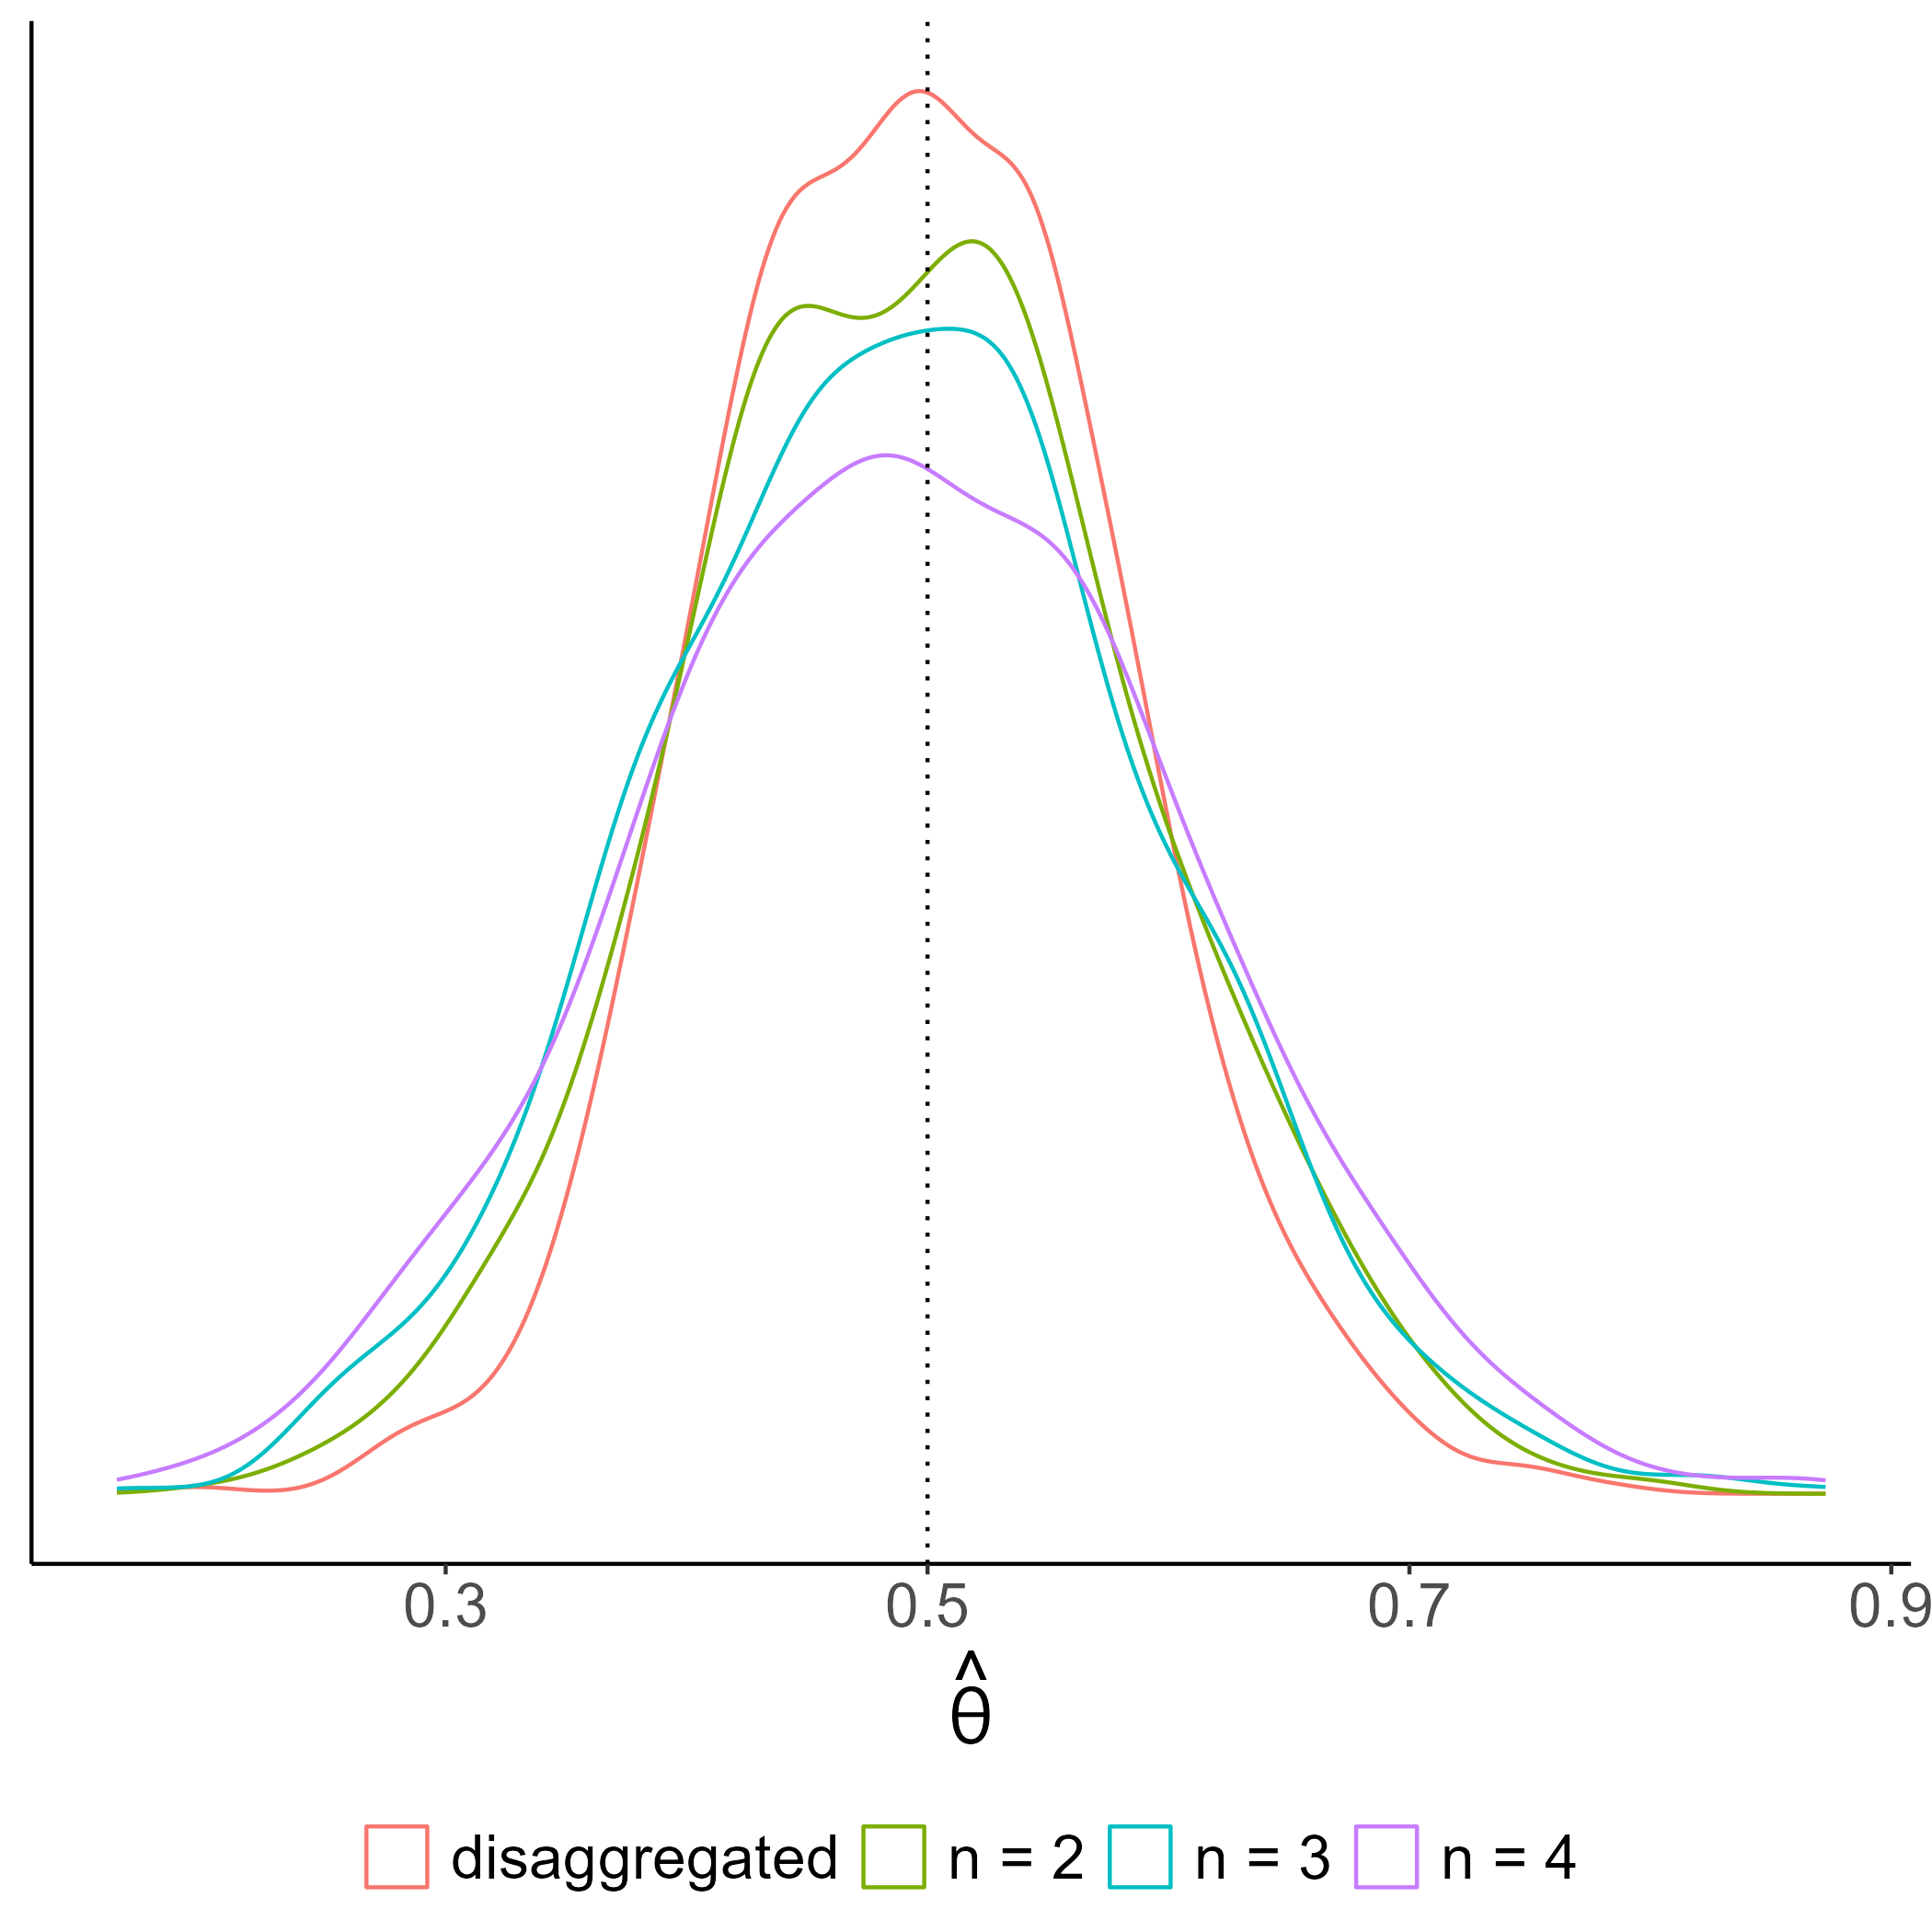
\includegraphics[width=1\linewidth]{figures/plot_mEstimates_noLag.png}
            \end{figure}
        \end{column}
        \begin{column}{.5\textwidth}
            \begin{table}[]
                \centering
                \begin{tabular}[t]{lrrr}
                    \toprule
                     $n$    & Avg. & Bias & MC-SE \\
                     \midrule
                    1 & 0.504 & 0.004 & 0.003 \\
                    2 & 0.505 & 0.005 & 0.003\\
                    3 & 0.503 & 0.003 & 0.003\\
                    4 & 0.505 & 0.005 & 0.004\\
                    \bottomrule
                \end{tabular}
                \caption{\footnotesize{Average estimate (Avg.), bias, and Monte Carlo standard errors (MC-SE) of the bias for the effect of the time-dependent predictor on the outcome. Based on 1000 replications. $n = 1$ denotes the disaggregated data.}}
            \end{table}
        \end{column}
    \end{columns}
\end{frame}

%--------------------
\subsection{AR(1)}
%--------------------

\begin{frame}{AR(1) | \textcite{hickman_effects_1972}}
    Suppose we have the disaggregate AR(1) process  $\bar{y}^{(3)}$
    \begin{equation}
        y_{t} = a y_{t-1} + u_{t},
    \end{equation}
    which, after applying the mean-aggregation scheme implies 
    \begin{equation}
        Y_{t} = a Y_{t - 1} + U_{t}.
    \end{equation}
    Repeated substitution results in
    \begin{equation}
        Y_{t} = a^{n} Y_{t - n} + U_{t} + a U_{t - 1} + a^{2} U_{t - 2} + ... + a^{n - 1} U_{t - n + 1}.
    \end{equation}
    We can then write the proper (nonoverlapping) aggregated model as 
    \begin{equation} \label{eq:aggregate_AR1}
        Y_{t} = A Y_{t - n} + V_{t},
    \end{equation}
    and compare $A$ with $a^{n}$. 
\end{frame}

%----

\begin{frame}{AR(1) | \textcite{hickman_effects_1972} II}
    \begin{quote}
        ``(...) it is misleading to say that because (1-13) and (1-14) agree except for the error term, they are the same model. The structure of the error term is very important for any estimation procedure and cannot be ignored in the specification of the model.''
    \end{quote}
    \begin{flushright} - \textcite{hickman_effects_1972} \end{flushright}
    \bigskip
    Ordinary least squares of Equation~\ref{eq:aggregate_AR1} is biased because the error term $V_{t}$ and the lagged regressor are correlated.     
\end{frame}

%----

\begin{frame}{AR(1) | OLS estimates of aggregated model ($n = 2$) I}
    Assuming a stationary process, the lag-$s$ autocovariance of an AR(1) process can be written as:
    \begin{equation}
        \text{plim} \frac{y'y_{-s}}{T} = a^{s} \sigma^{2}_{y}. 
    \end{equation}
    The OLS-estimate of the aggregated model is $\hat{A}$
    \begin{equation}
        \hat{A} = (Y_{-n} ' Y_{-n})^{-1}(Y_{-n} ' Y),
    \end{equation}
    which can rewritten (by covariance stationarity) to
    \begin{equation}
        \hat{A} = (Y'Y)^{-1}(Y_{-3}'Y),
    \end{equation}
    and in the limit ($T \rightarrow \infty$) is equal to
    \begin{equation} 
         \text{plim} \; \hat{A} = \frac{\text{plim} \; Y_{-3}'Y}{\text{plim} \; Y'Y}
    \end{equation}
\end{frame}

%----

\begin{frame}{AR(1) | OLS estimates of aggregated model ($n = 2$) II}
    For aggregation of $n = 2$ periods, we can write: 
    \begin{align}
        \text{plim} \; \hat{A}^{(2)} &= \frac{\text{plim} \; (y_{-2} + y_{-3})'(y + y_{-1})}{\text{plim} \; (y + y_{-1})'(y + y_{-1})} \\
        &= \frac{\text{plim} \; (y'y_{-2} + y_{-1}'y_{-2} + y'y_{-3} + y_{-1}'y_{-3})}{\text{plim} \; (y^{2} + 2y'y_{-1} + y^{2}_{-1})}\\
        &= \frac{a + 2 a^{2} + a^{3}}{2 + 2a}\\
        &= \frac{1 + 2a + a^{2}}{2 + 2a}a
    \end{align}
    When $-1 < a < 1$, the numerator is smaller than the denominator, and $\hat{A}^{(2)} < a$
\end{frame}

%----

\begin{frame}{AR(1) | OLS estimates of aggregated model ($n = 3$)}
    For aggregation of $n = 3$ periods: 
    \begin{align}
        \text{plim} \; \hat{A}^{(3)} &= \frac{\text{plim} (y_{-3} + y_{-4} + y_{-5})'(y + y_{-1} + y_{-2})}{\text{plim} (y + y_{-1} + y_{-2})'(y + y_{-1} + y_{-2})}\\
        &= \frac{a + 2a^{2} + 3a^{3} + 2a^{4} + a^{5}}{3 + 4a + 2a^{2}}\\
        &= \frac{(3a^{3}) + (2a^{2} + 2a^{4}) + (a + a^{5})}{3a^{3} + 4a^{4} + 2a^{5}} a^{3} \label{eq:bias_n3_AR1}
    \end{align}
    \textcite{hickman_effects_1972} use this grouping of terms to show that $\hat{A}^{(3)} > a^{3}$. 
\end{frame}

%----

\begin{frame}{AR(1) | OLS estimates of aggregated model ($n = 4$)}
    For aggregation of $n = 4$ periods: 
    \begin{align}
        \text{plim} \; \hat{A}^{(4)} &= \frac{\text{plim} (y_{-4} + y_{-5} + y_{-6} + y_{-7})'(y + y_{-1} + y_{-2} + y_{-3})}{\text{plim} (y + y_{-1} + y_{-2} + y_{-3})'(y + y_{-1} + y_{-2} + y_{-3})}\\
        &= \frac{a + 2a^{2} + 3a^{3} + 4a^{4} + 3a^{5} + 2a^{6} + a^{7}}{4 + 6a + 4a^{2} + 2a^{3}}
    \end{align}
    \bigskip
    For aggregation of $n = 6$ periods: 
    \footnotesize{
        \begin{align}
            \text{plim} \; \hat{A}^{(6)} &= \frac{\text{plim} (y_{-6} + y_{-7} + y_{-8} + y_{-9} + y_{-10} + y_{-11})'(y + y_{-1} + y_{-2} + y_{-3} + y_{-4} + y_{-5})}{\text{plim} (y + y_{-1} + y_{-2} + y_{-3} + y_{-4} + y_{-5})'(y + y_{-1} + y_{-2} + y_{-3} + y_{-4} + y_{-5})}\\
            &= \frac{a + 2a^{2} + 3a^{3} + 4a^{4} + 5a^{5} + 6a^{6} + 5a^{7} + 4a^{8} + 3a^{9} + 2a^{10} + a^{11}}{6 + 10a + 8a^{2} + 6a^{3} + 4a^{4} + 2a^{5}}
        \end{align}
    }
\end{frame}

%----

\begin{frame}{AR(1) | OLS estimates $\hat{A}$ for $n \rightarrow \infty$}
    \begin{figure}
        \centering
        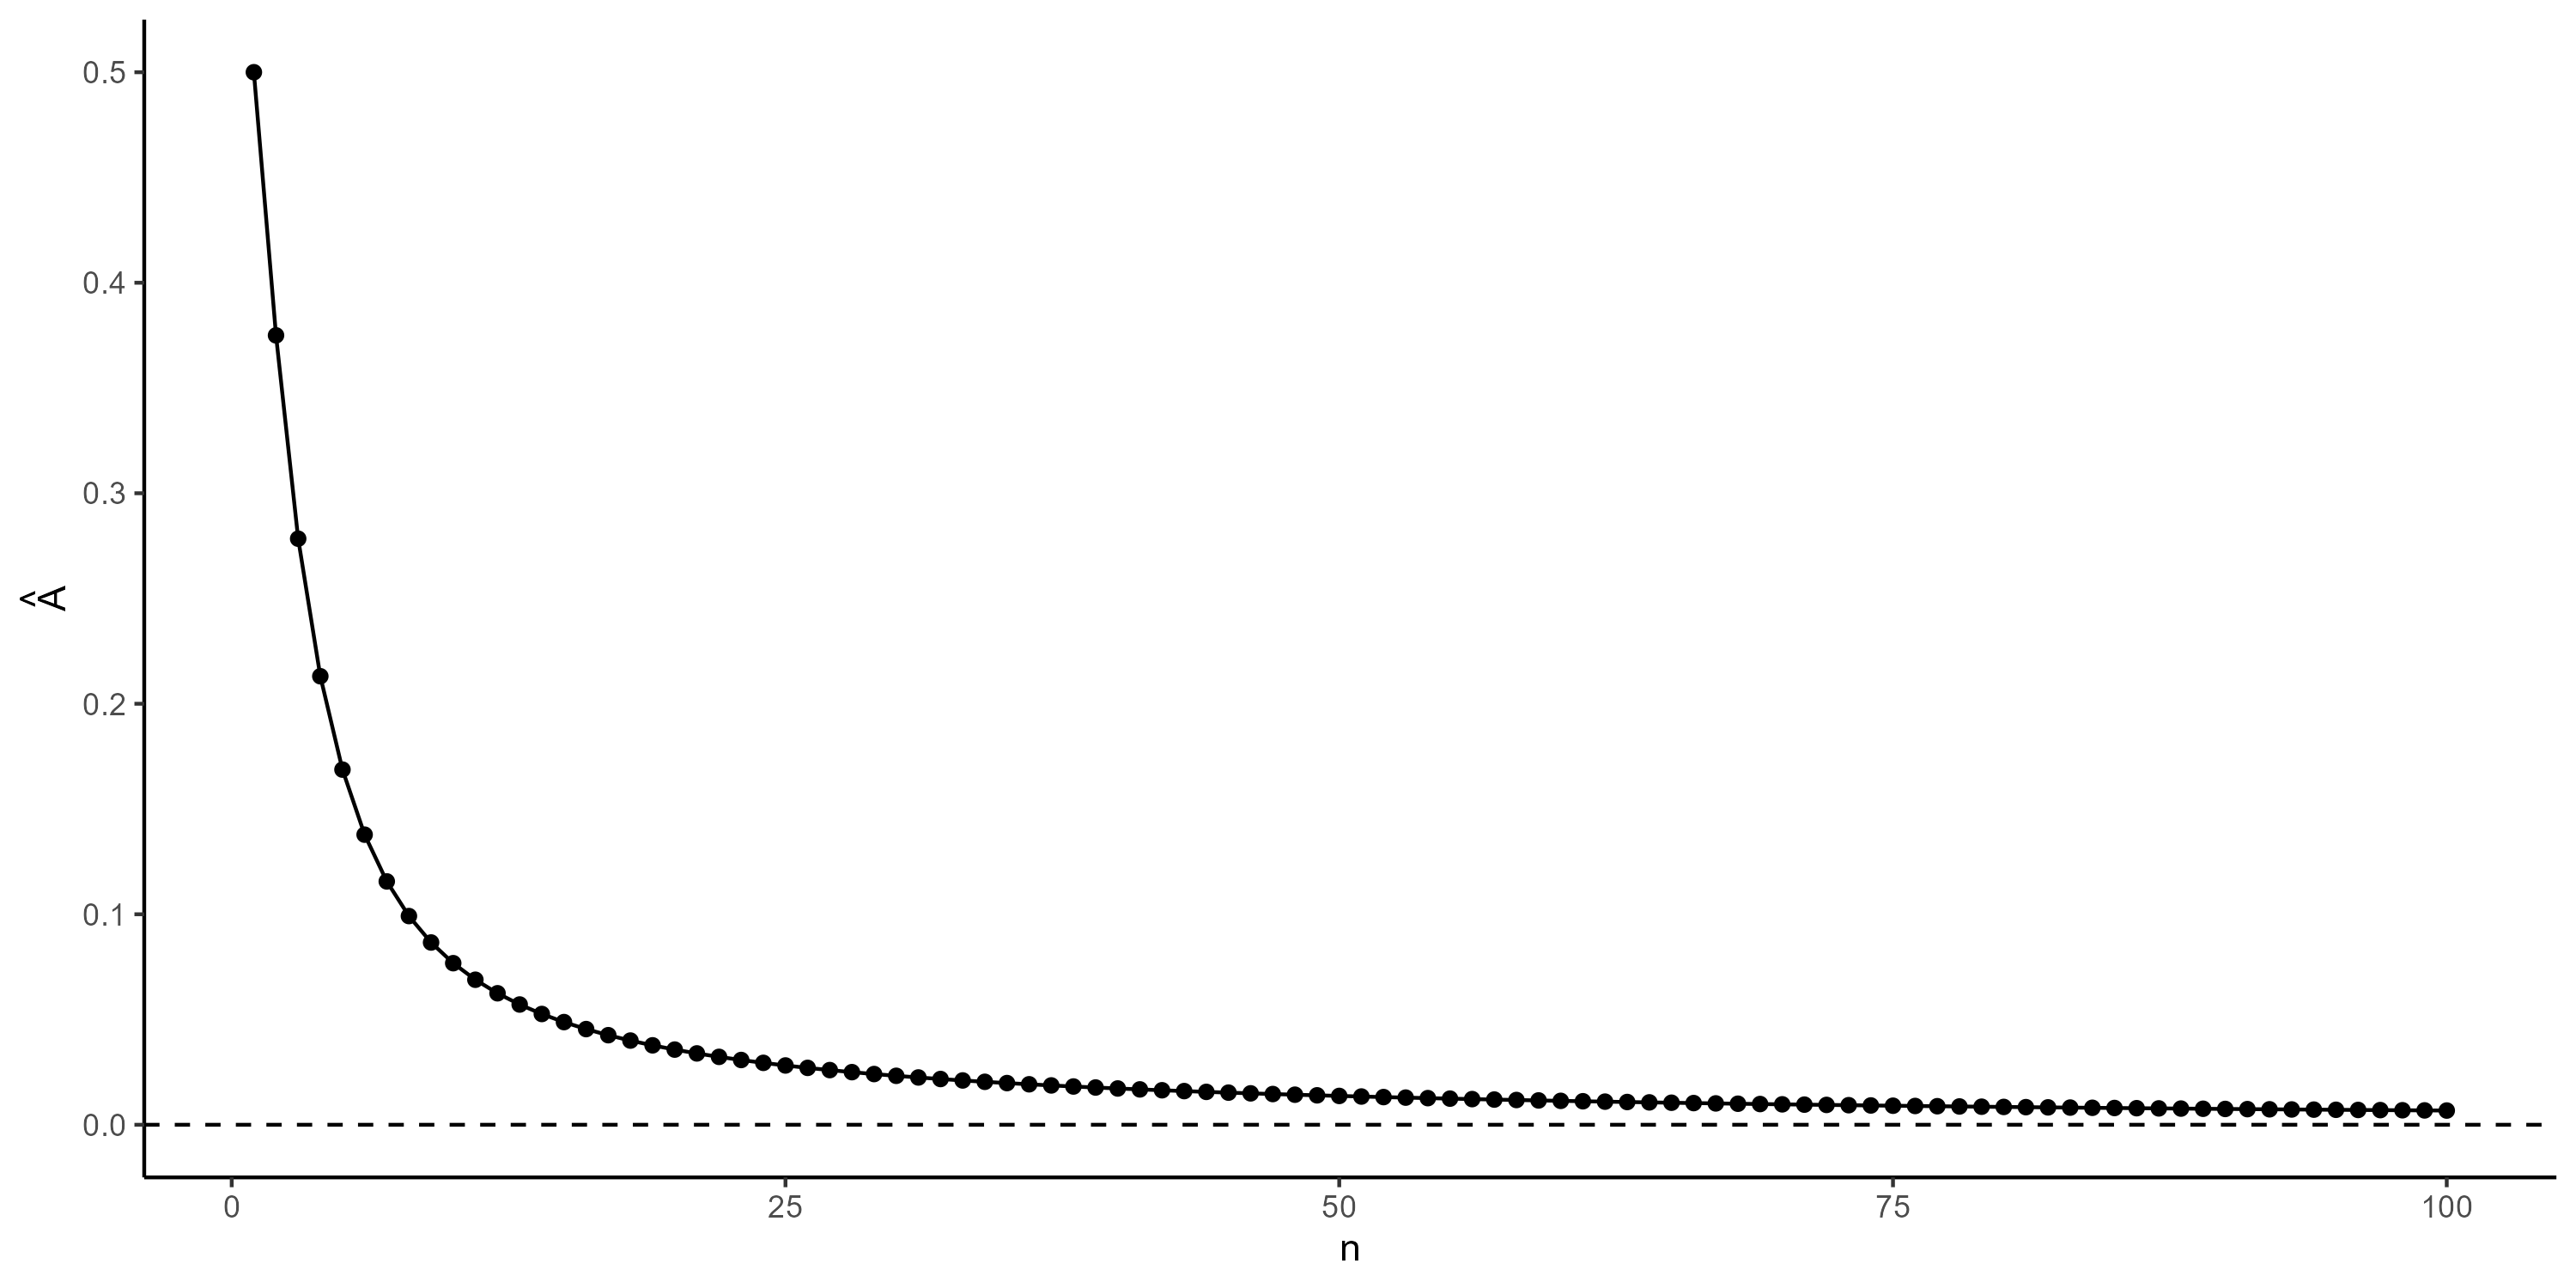
\includegraphics[width=1\linewidth]{figures/plot_AHat_nToInf.png}
    \end{figure}
\end{frame}

%----

\begin{frame}{AR(1) | Data file ($n = 2$)}
    \footnotesize
    \begin{table}[]
        \centering
        \begin{tabular}{ccc}
            \toprule
            Y & t & unit \\
            \midrule
            \textcolor{red}{0.18} & 1 & 1 \\
            \textcolor{red}{-0.66} & 2 & 1 \\
            \textcolor{green}{0.52} & 3 & 1\\
            \textcolor{green}{0.43} & 4 & 1 \\
            \textcolor{blue}{1.41} & 5 & 1 \\
            \textcolor{blue}{1.33} & 6 & 1 \\
            \bottomrule
        \end{tabular}
        \caption{First six rows of disaggregated data.}
    \end{table} \\
    \bigskip
    \begin{table}[ht]
        \centering
        \begin{tabularx}{.39\linewidth}{ccccc}
            \toprule
            Y & t & unit & frame & Y\_mean \\
            \midrule
            -0.66 & 2 & 1 & 1 & \textcolor{red}{-0.24} \\
            0.43 & 4 & 1 & 2 & \textcolor{green}{0.48} \\
            0.33 & 6 & 1 & 3 & \textcolor{blue}{1.37} \\
            \bottomrule
        \end{tabularx}
        \caption{Corresponding aggregated data ($n = 2$).}
    \end{table}
\end{frame}

%----

\begin{frame}{AR(1) | Data visualization ($n = 4$)}
    \begin{figure}
        \centering
        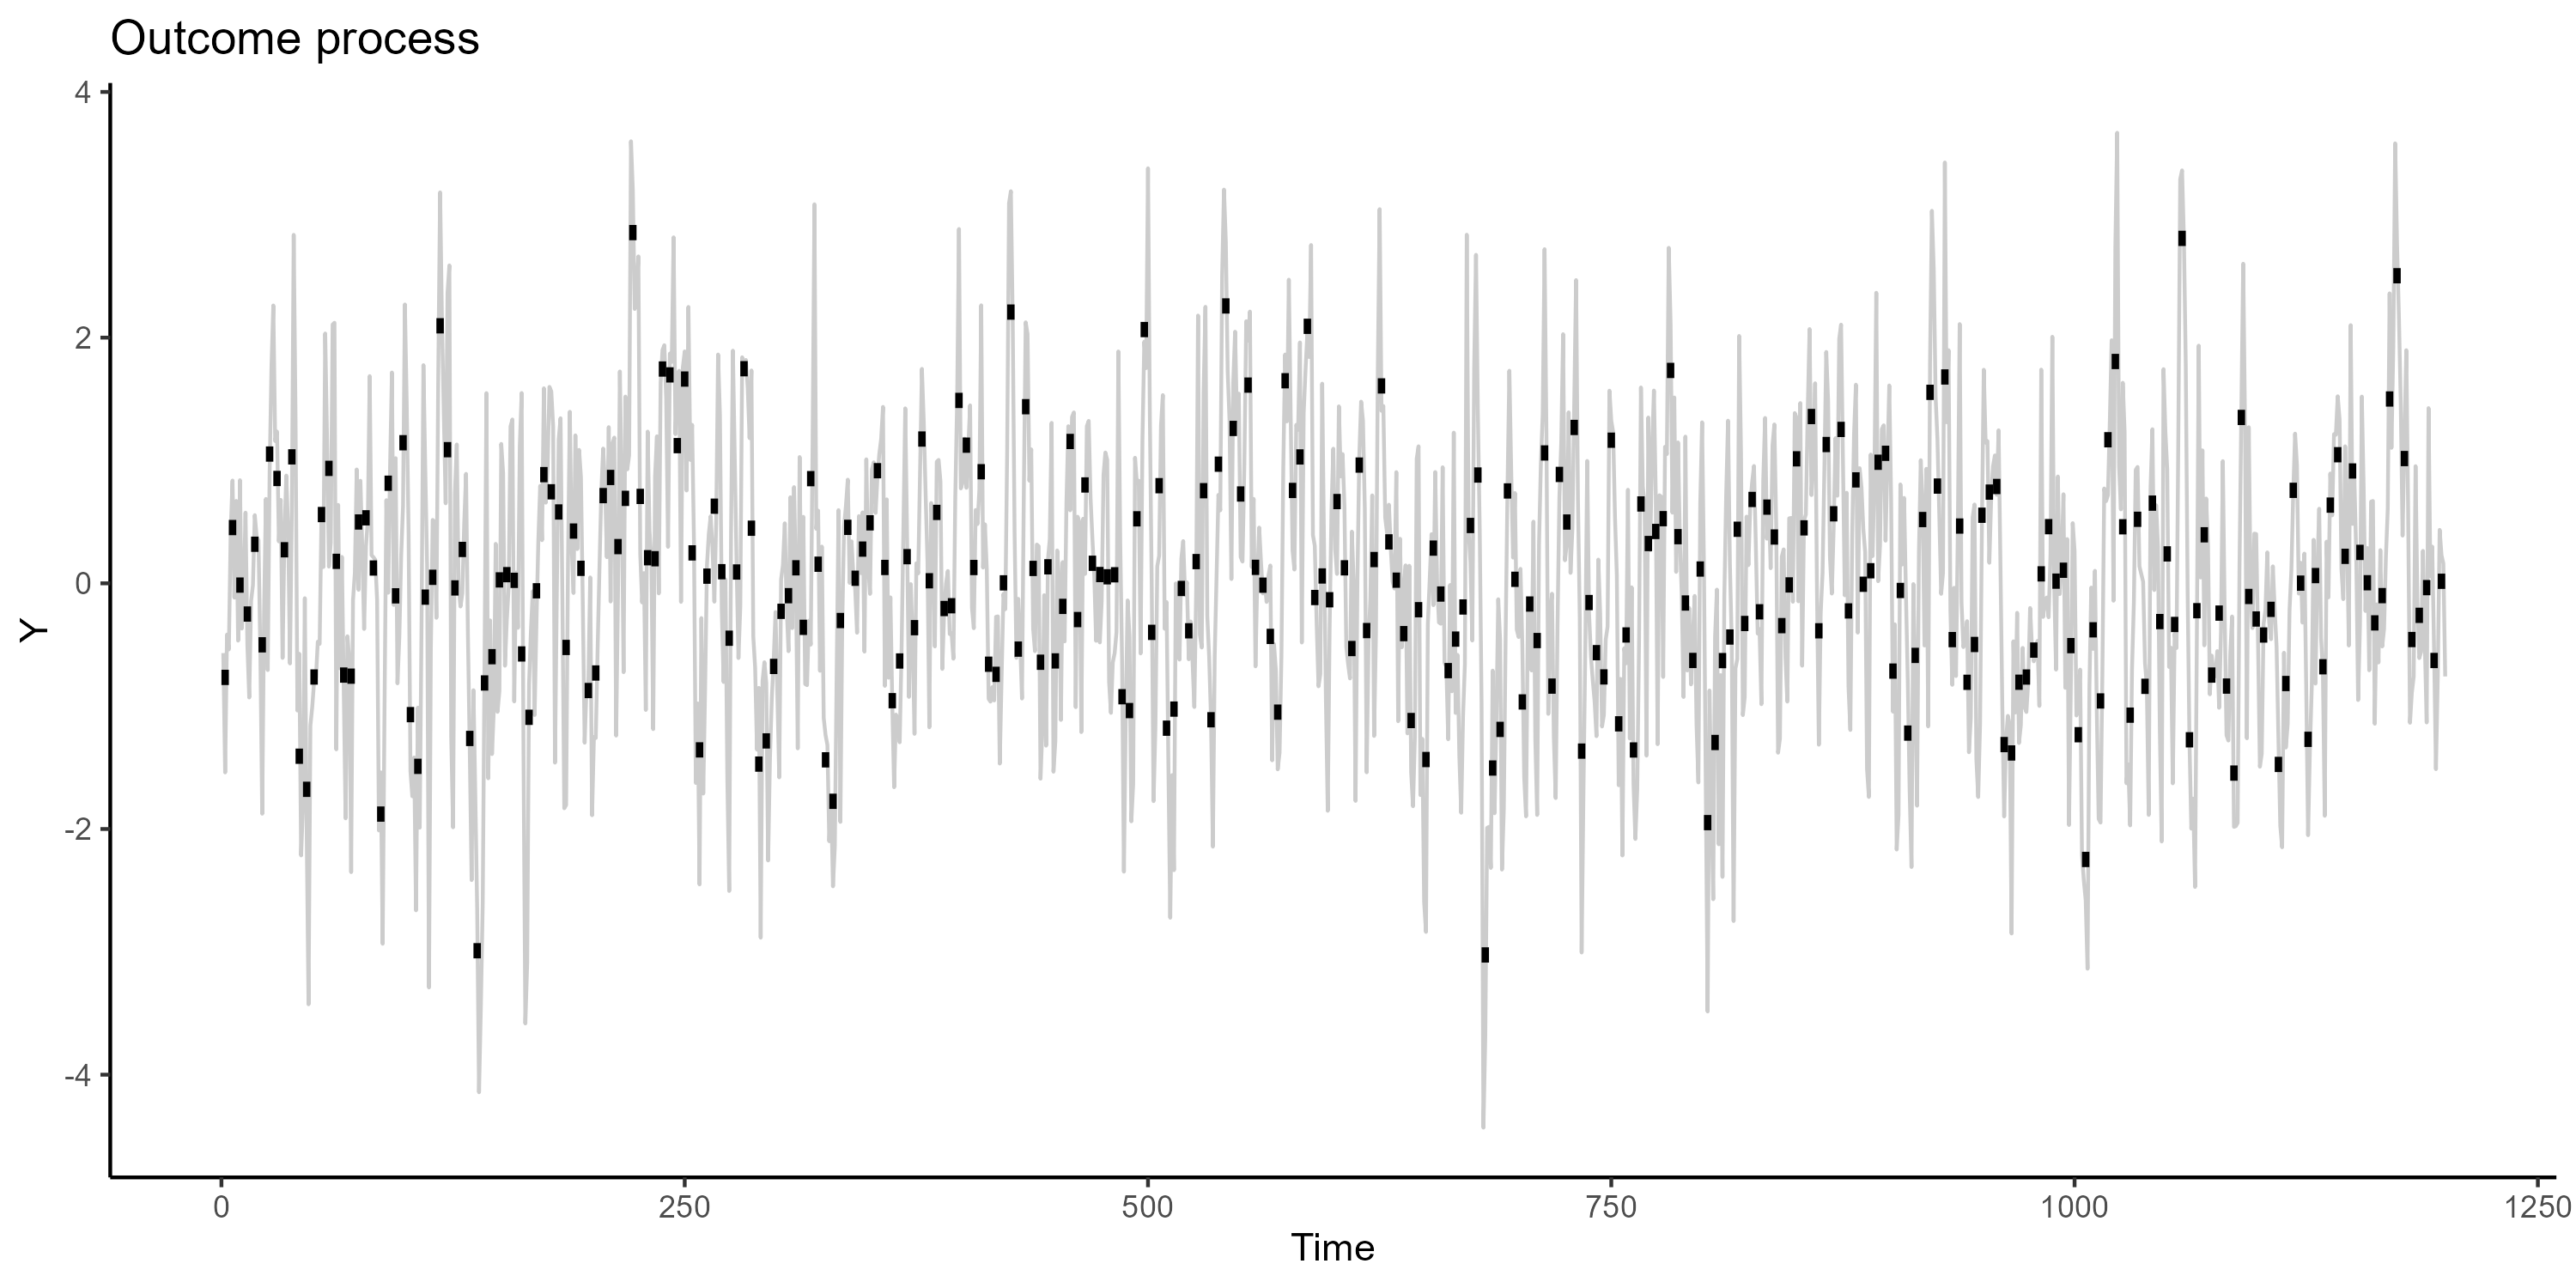
\includegraphics[width=1\linewidth]{figures/plot_singleSubject_AR1.png}
    \end{figure}
\end{frame}

%----

\begin{frame}{AR(1) | Results AR(1) model (sampling distribution)}
    \begin{columns}
        \begin{column}{.5\textwidth}
            \begin{figure}
                \centering
                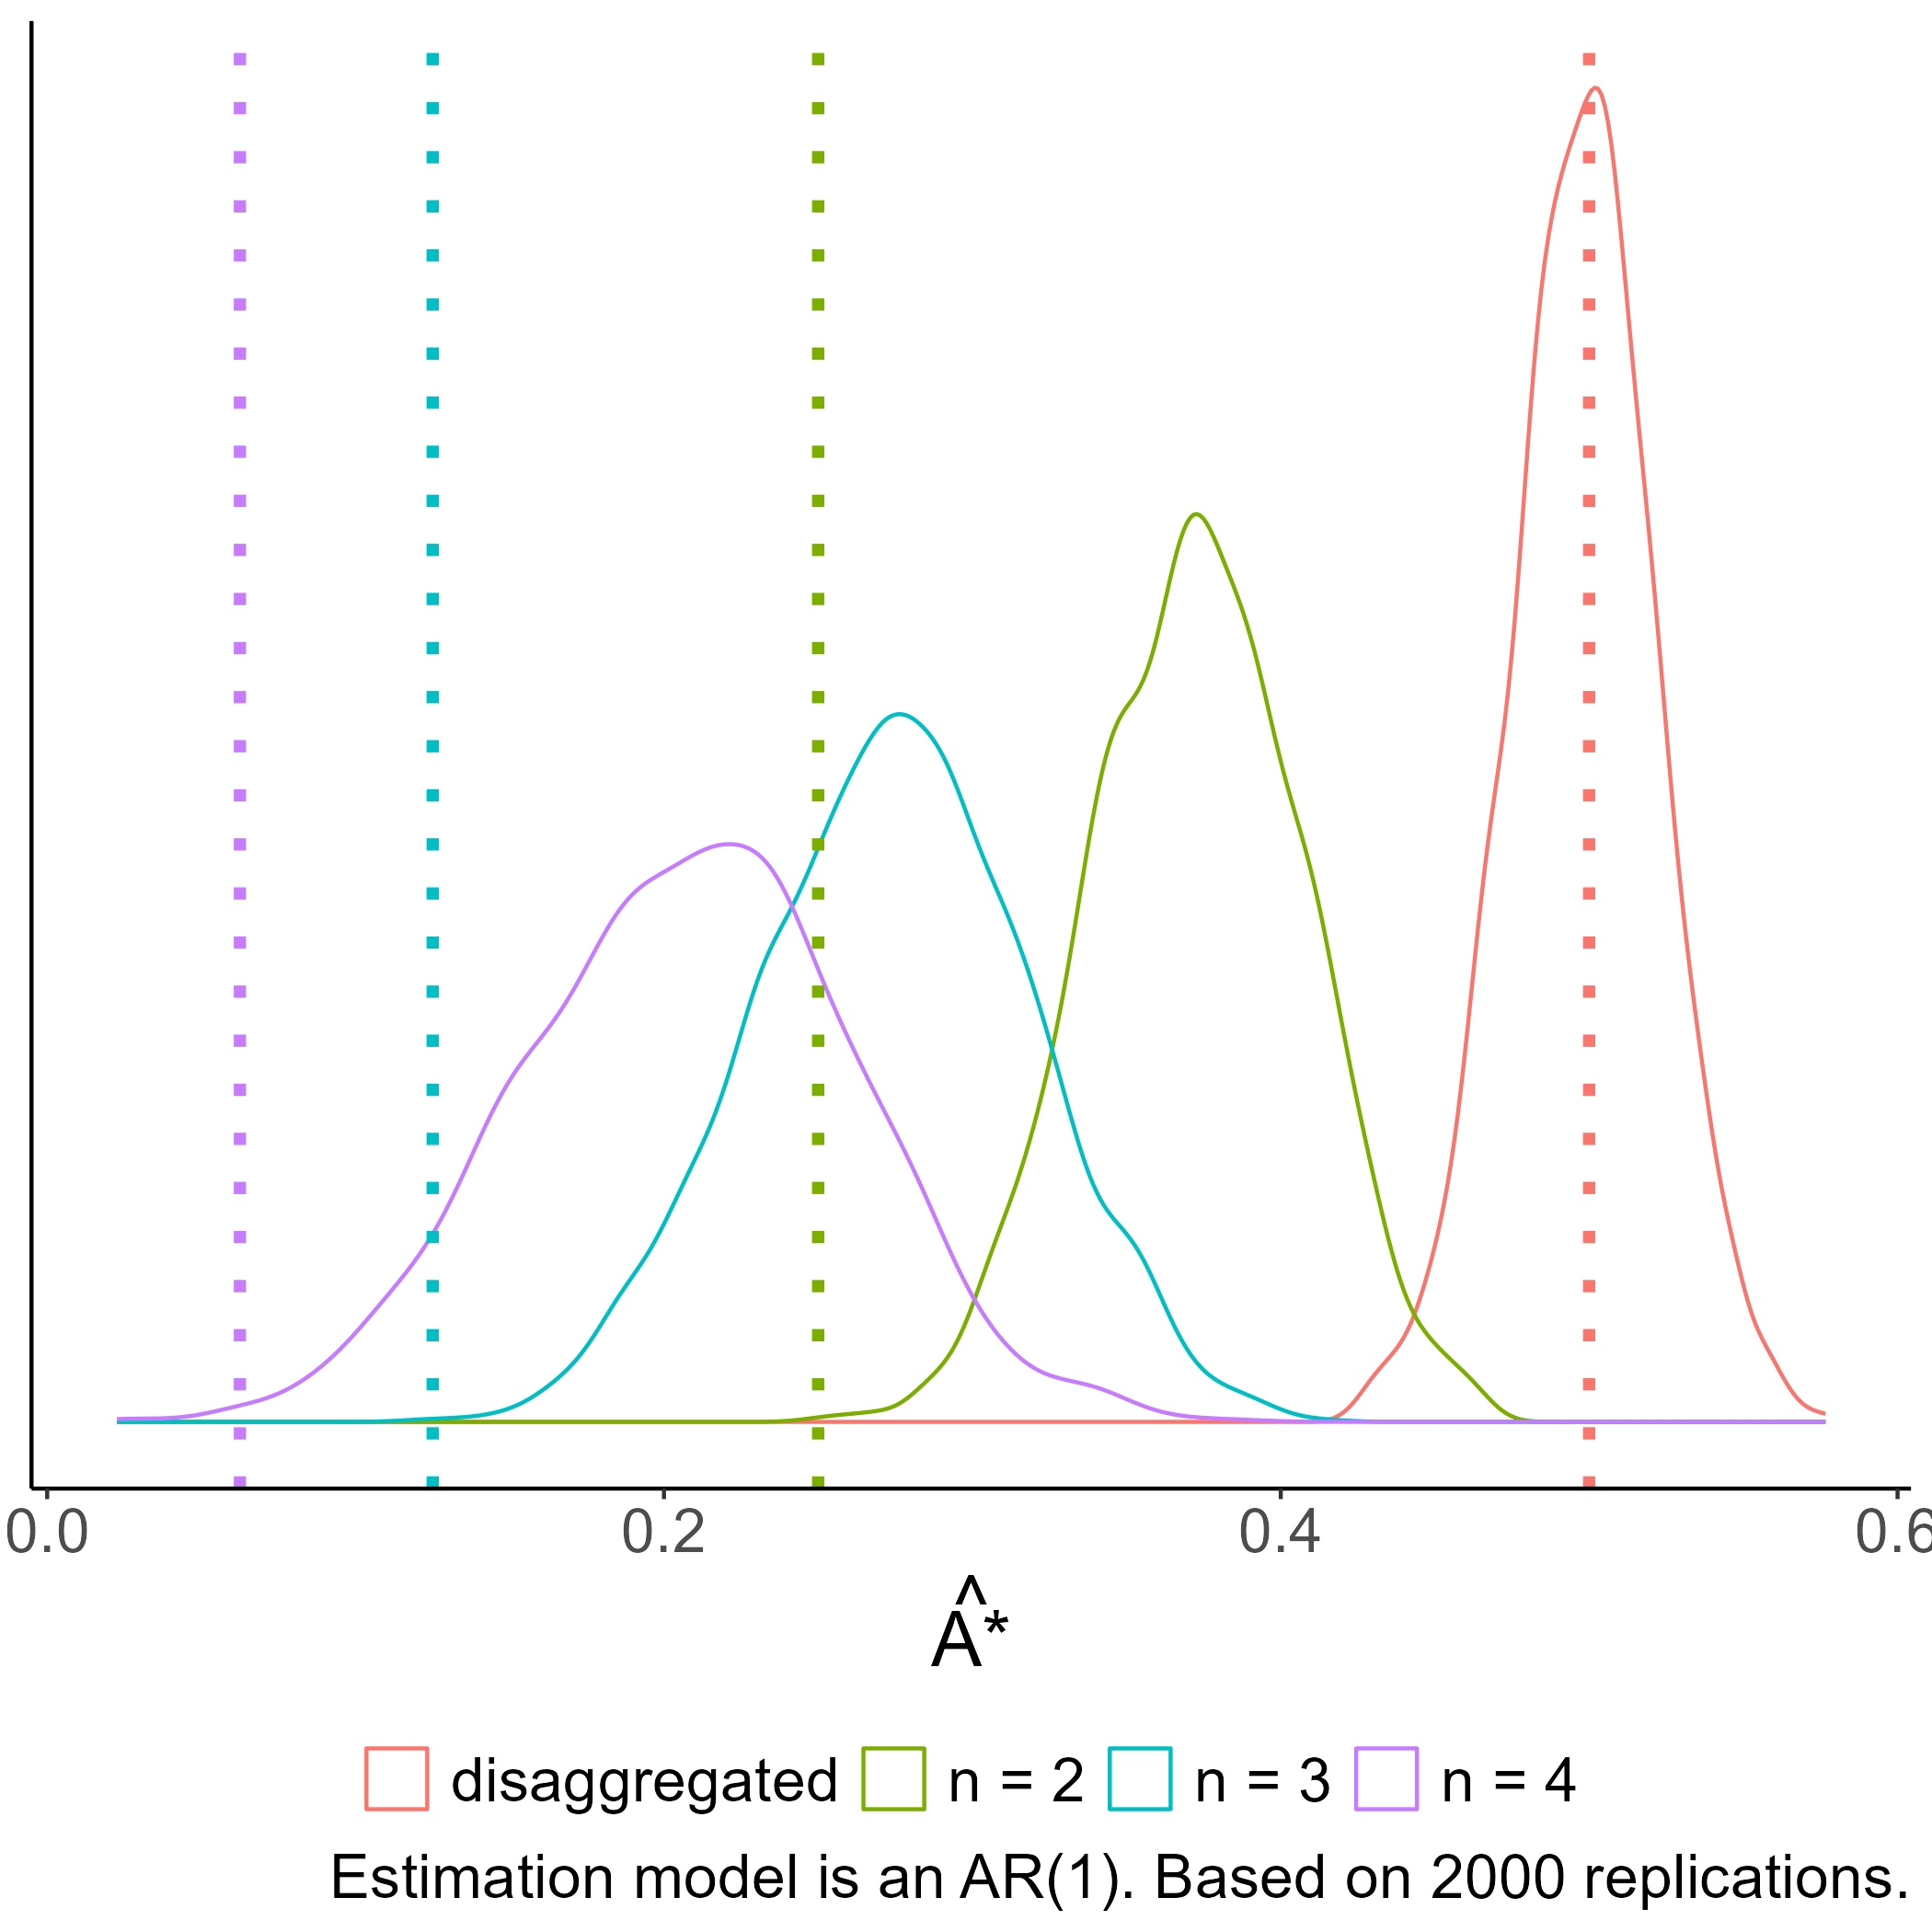
\includegraphics[width=1\linewidth]{figures/plot_AStarEstimates_AR1.png}
            \end{figure}
        \end{column}
        \begin{column}{.5\textwidth}
            \begin{table}[]
                \centering
                \begin{tabular}[t]{lrrr}
                    \toprule
                     $n$    & Avg. & Bias & MC-SE \\
                     \midrule
                    1 & 0.498 & -0.002 & 0.001 \\
                    2 & 0.372 & 0.122 & 0.001\\
                    3 & 0.274 & 0.149 & 0.001\\
                    4 & 0.208 & 0.145 & 0.001\\
                    \bottomrule
                \end{tabular}
                \caption{\footnotesize{Average estimate (Avg.), bias, and Monte Carlo standard errors (MC-SE) of the bias for the autoregressive effect, estimated using an AR(1) model. Based on 2000 replications. $n = 1$ denotes the disaggregated data. Dividing the average estimate for $n = 3$ by the bias term of Equation~\ref{eq:bias_n3_AR1} results in $0.123$.}}
            \end{table}
        \end{column}
    \end{columns}
\end{frame}

%----

\begin{frame}{AR(1) | Results ARMA(1,1) model (sampling distribution)}
    \begin{columns}
        \begin{column}{.5\textwidth}
            \begin{figure}
                \centering
                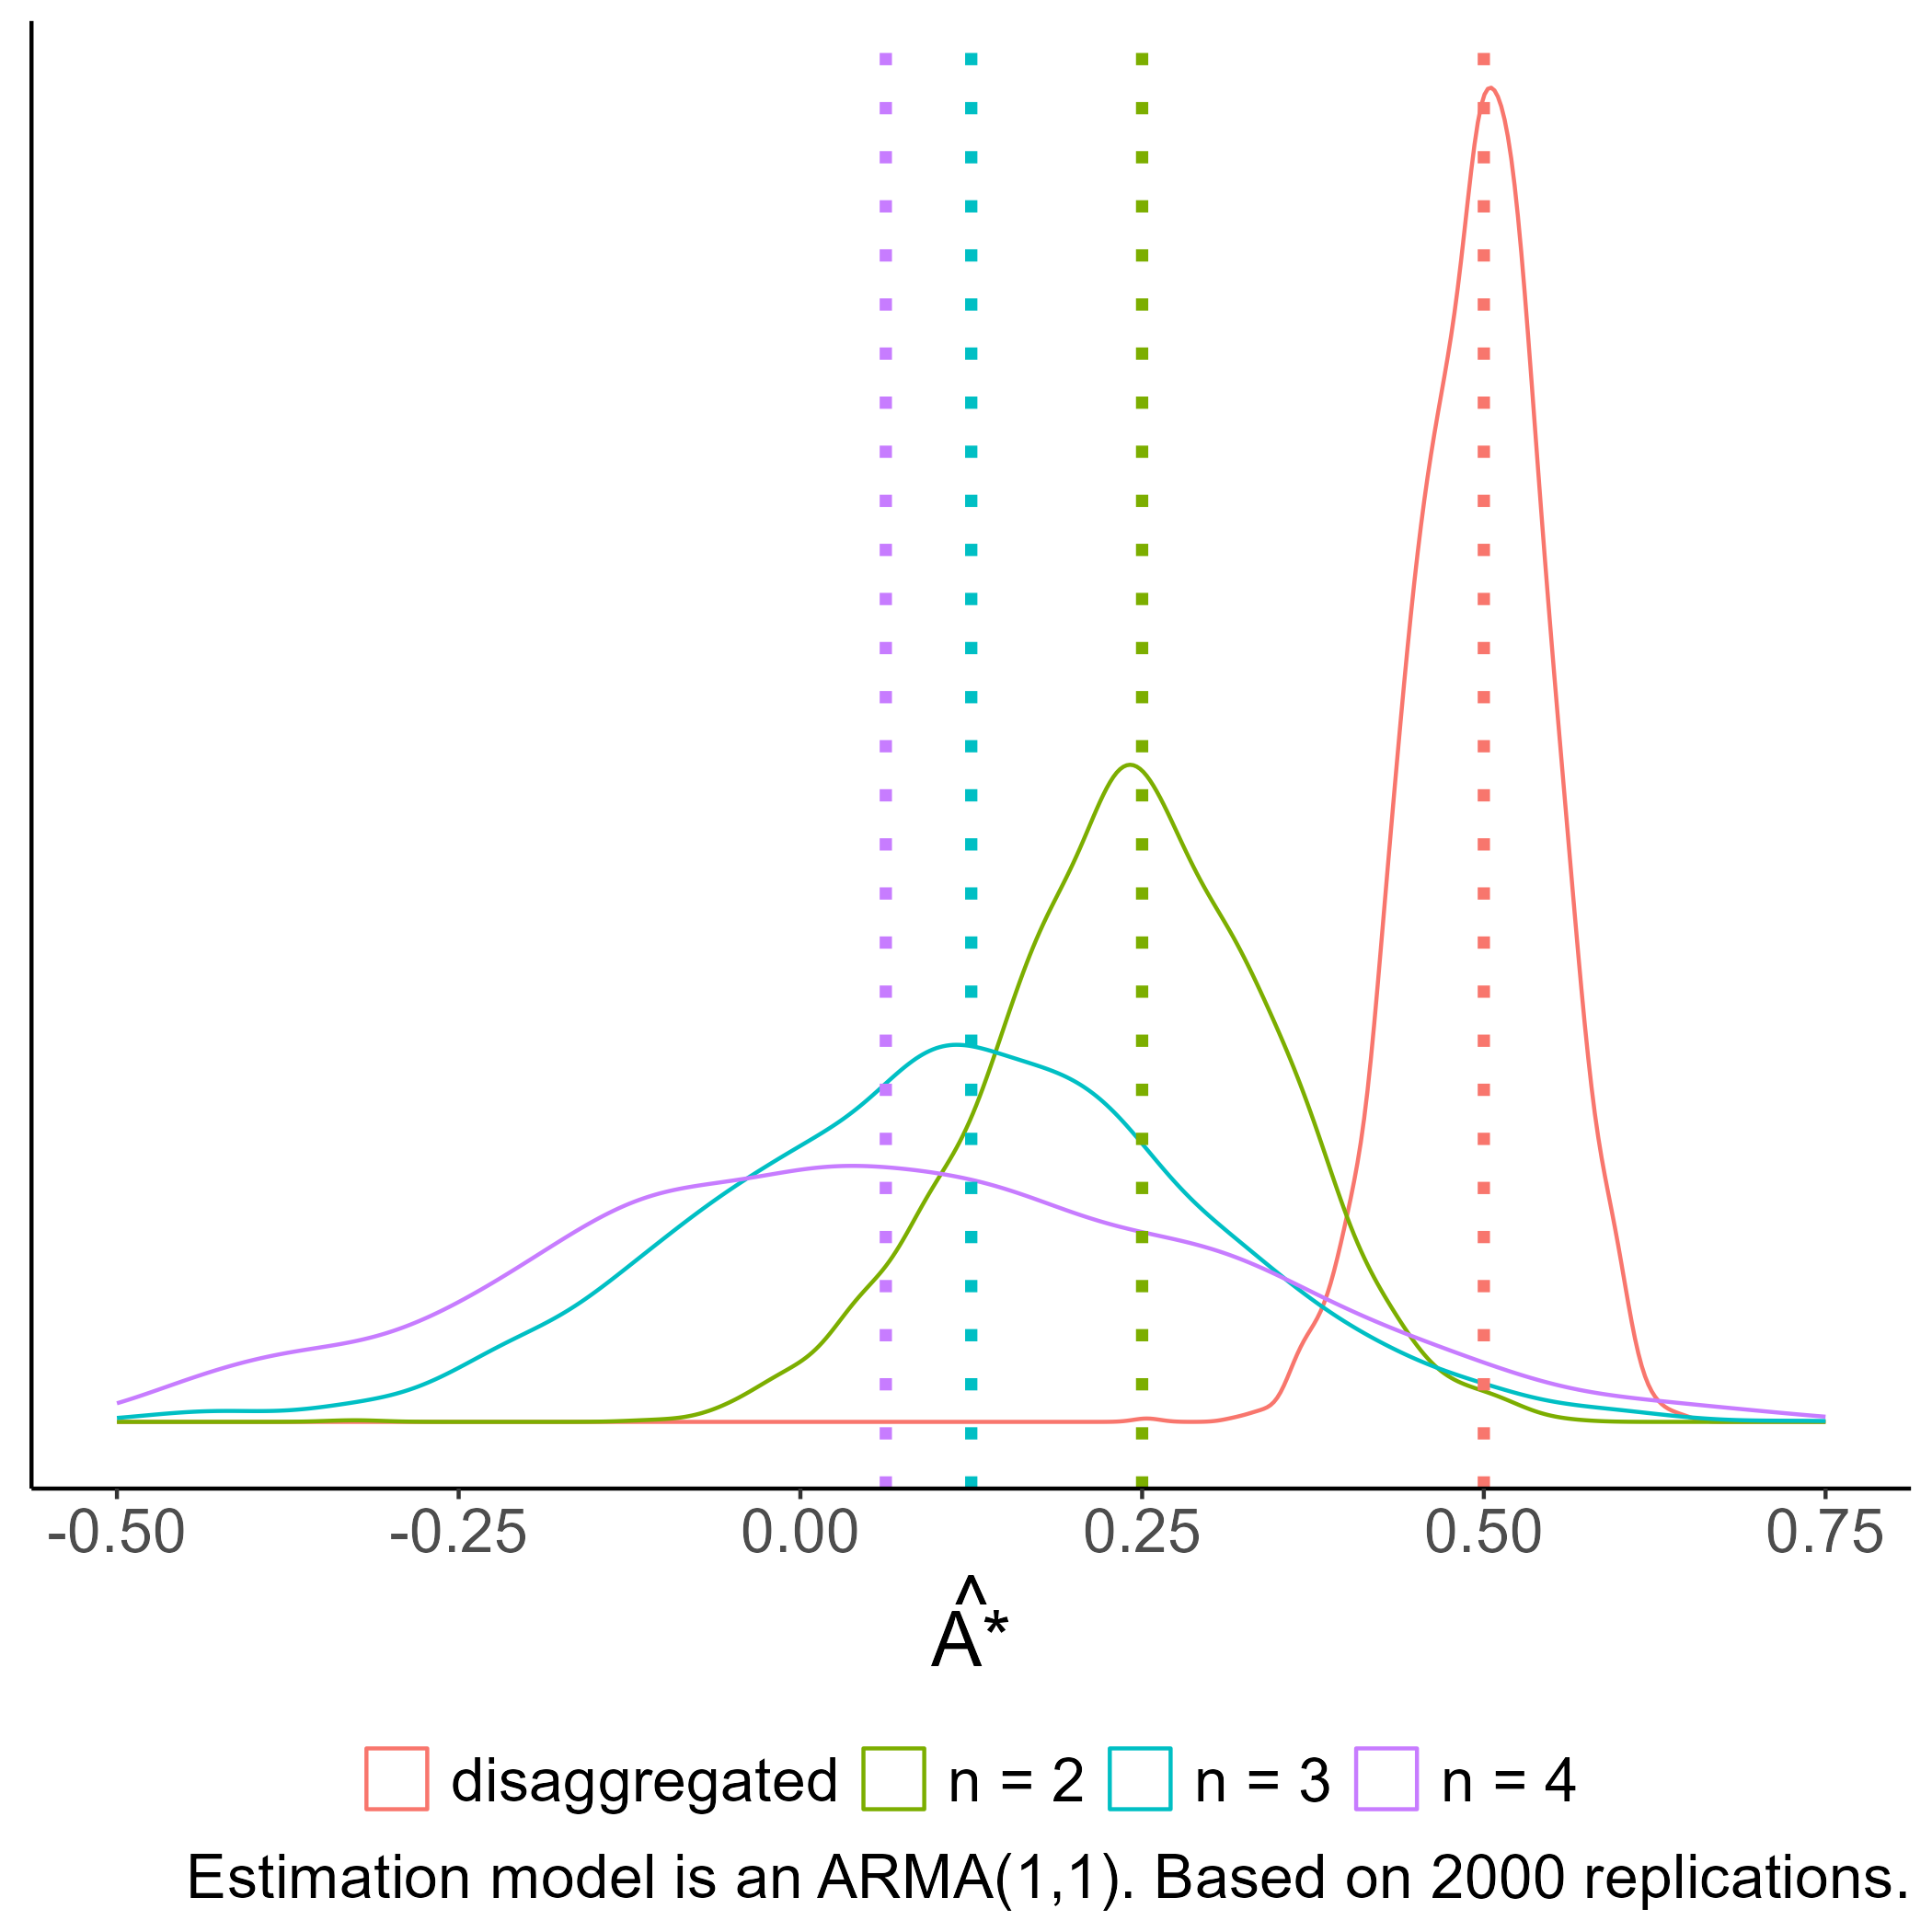
\includegraphics[width=1\linewidth]{figures/plot_AStarEstimates_ARMA11.png}
            \end{figure}
        \end{column}
        \begin{column}{.5\textwidth}
            \begin{table}[]
                \centering
                \begin{tabular}[t]{lrrr}
                    \toprule
                     $n$    & Avg. & Bias & MC-SE \\
                     \midrule
                    1 & 0.496 & -0.004 & 0.001 \\
                    2 & 0.240 & -0.010 & 0.002\\
                    3 & 0.109 & -0.016 & 0.004\\
                    4 & 0.044 & -0.019 & 0.006\\
                    \bottomrule
                \end{tabular}
                \caption{\footnotesize{Average estimate (Avg.), bias, and Monte Carlo standard errors (MC-SE) of the bias for the autoregressive effect, estimated using an AR(1) model. Based on 2000 replications. $n = 1$ denotes the disaggregated data.}}
            \end{table}
        \end{column}
    \end{columns}
\end{frame}

%----

\begin{frame}{ARX(1) | \textcite{hickman_effects_1972} I}
    Combining time-dependent predictors with lagged effects, we get
    \begin{equation}
        Y = AY_{-n} + BX + V. 
    \end{equation}
    Using spectral density representation, the plim of the autoregressive parameter is:\\
    \bigskip
    \begin{figure}
        \centering
        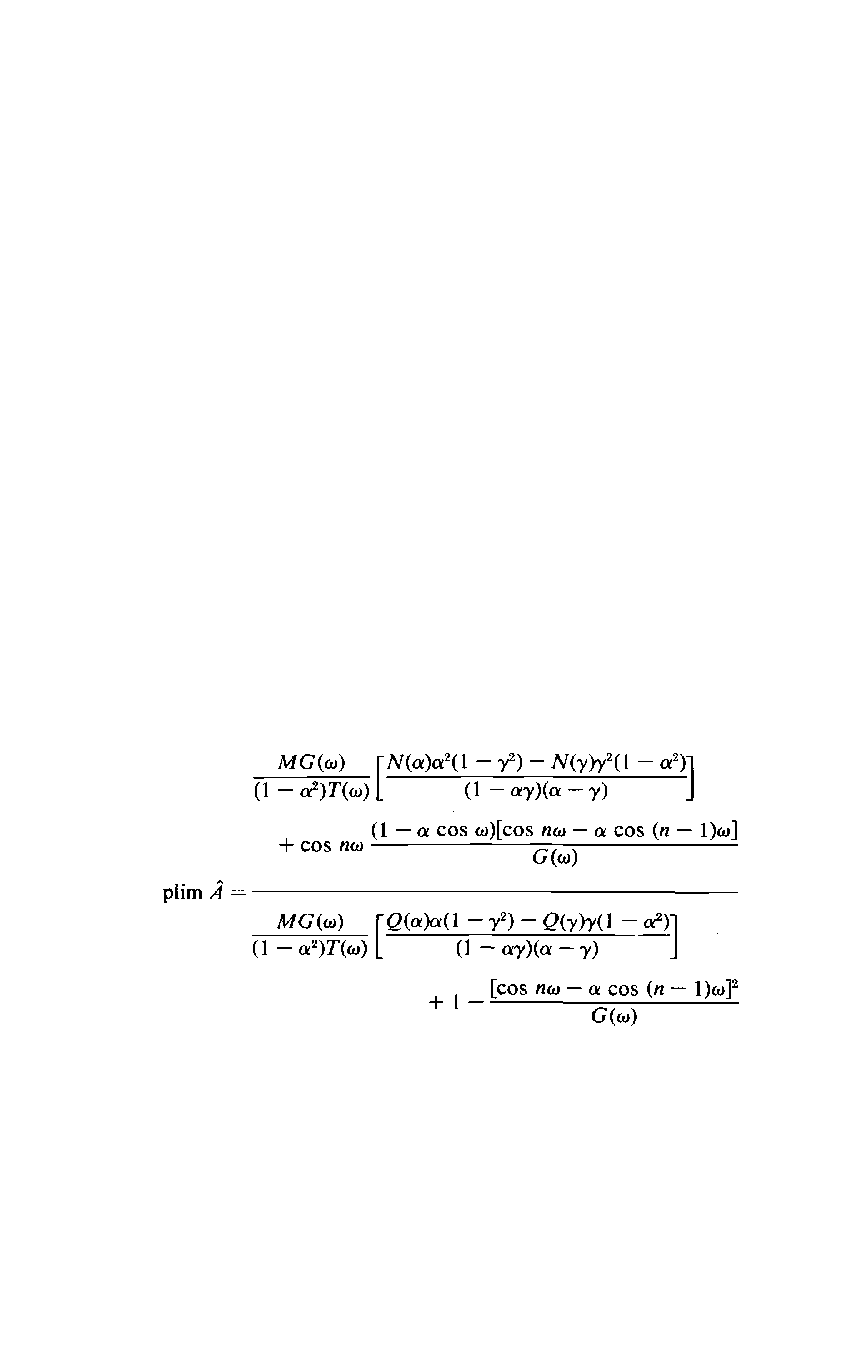
\includegraphics[width=0.6\linewidth]{figures/equation_ARX1_aggregation.pdf}
    \end{figure}
\end{frame}

%----

\begin{frame}{ARX(1) | \textcite{hickman_effects_1972} II}
    \textcite{hickman_effects_1972} also derive the plim of the estimator $\hat{B}$.\\
    \bigskip
    Under the assumption that variance is mainly ``trend-driven'' (i.e., long-term), they derive:
    \begin{equation}
        \text{plim} \hat{B} = \frac{\beta}{1 - a}[1 - \text{plim}\hat{A}]
    \end{equation}
    Concerning the plim of $\hat{A}$ (and by extension, also for $\hat{B}$), \textcite{hickman_effects_1972} state: \\
    \bigskip
    \begin{quote}
        ``This relationship is so complicated that no general tendencies can be observed until simplifying approximations are made.''
    \end{quote}
\end{frame}

%----

\begin{frame}{ARX(1) | Data file ($n = 2$)}
    \footnotesize
    \begin{table}[]
        \centering
        \begin{tabular}{cccc}
            \toprule
            chi & Y & t & unit \\
            \midrule
            1 & \textcolor{red}{0.18} & 1 & 1 \\
            1 & \textcolor{red}{-0.66} & 2 & 1 \\
            1 & \textcolor{green}{0.52} & 3 & 1 \\
            1 & \textcolor{green}{0.43} & 4 & 1 \\
            1 & \textcolor{blue}{1.41} & 5 & 1 \\
            0 & \textcolor{blue}{1.33} & 6 & 1 \\
            \bottomrule
        \end{tabular}
        \caption{First six rows of disaggregated data.}
    \end{table} \\
    \bigskip
    \begin{table}[ht]
        \centering
        \begin{tabularx}{.6\linewidth}{ccccccc}
            \toprule
            chi & Y & t & unit & frame & chi\_mean & Y\_mean \\
            \midrule
            1 & -0.66 & 2 & 1 & 1 & 1.0 & \textcolor{red}{-0.24} \\
            1 & 0.43 & 4 & 1 & 2 & 1.0 & \textcolor{green}{0.48}\\
            0 & 1.33 & 6 & 1 & 3 & 0.5 & \textcolor{blue}{1.37} \\
            \bottomrule
        \end{tabularx}
        \caption{Corresponding aggregated data ($n = 2$).}
    \end{table}
\end{frame}

%----

\begin{frame}{ARX(1) | Results ARX(1) model (sampling distribution $\hat{M}$)}
    \begin{columns}
        \begin{column}{.5\textwidth}
            \begin{figure}
                \centering
                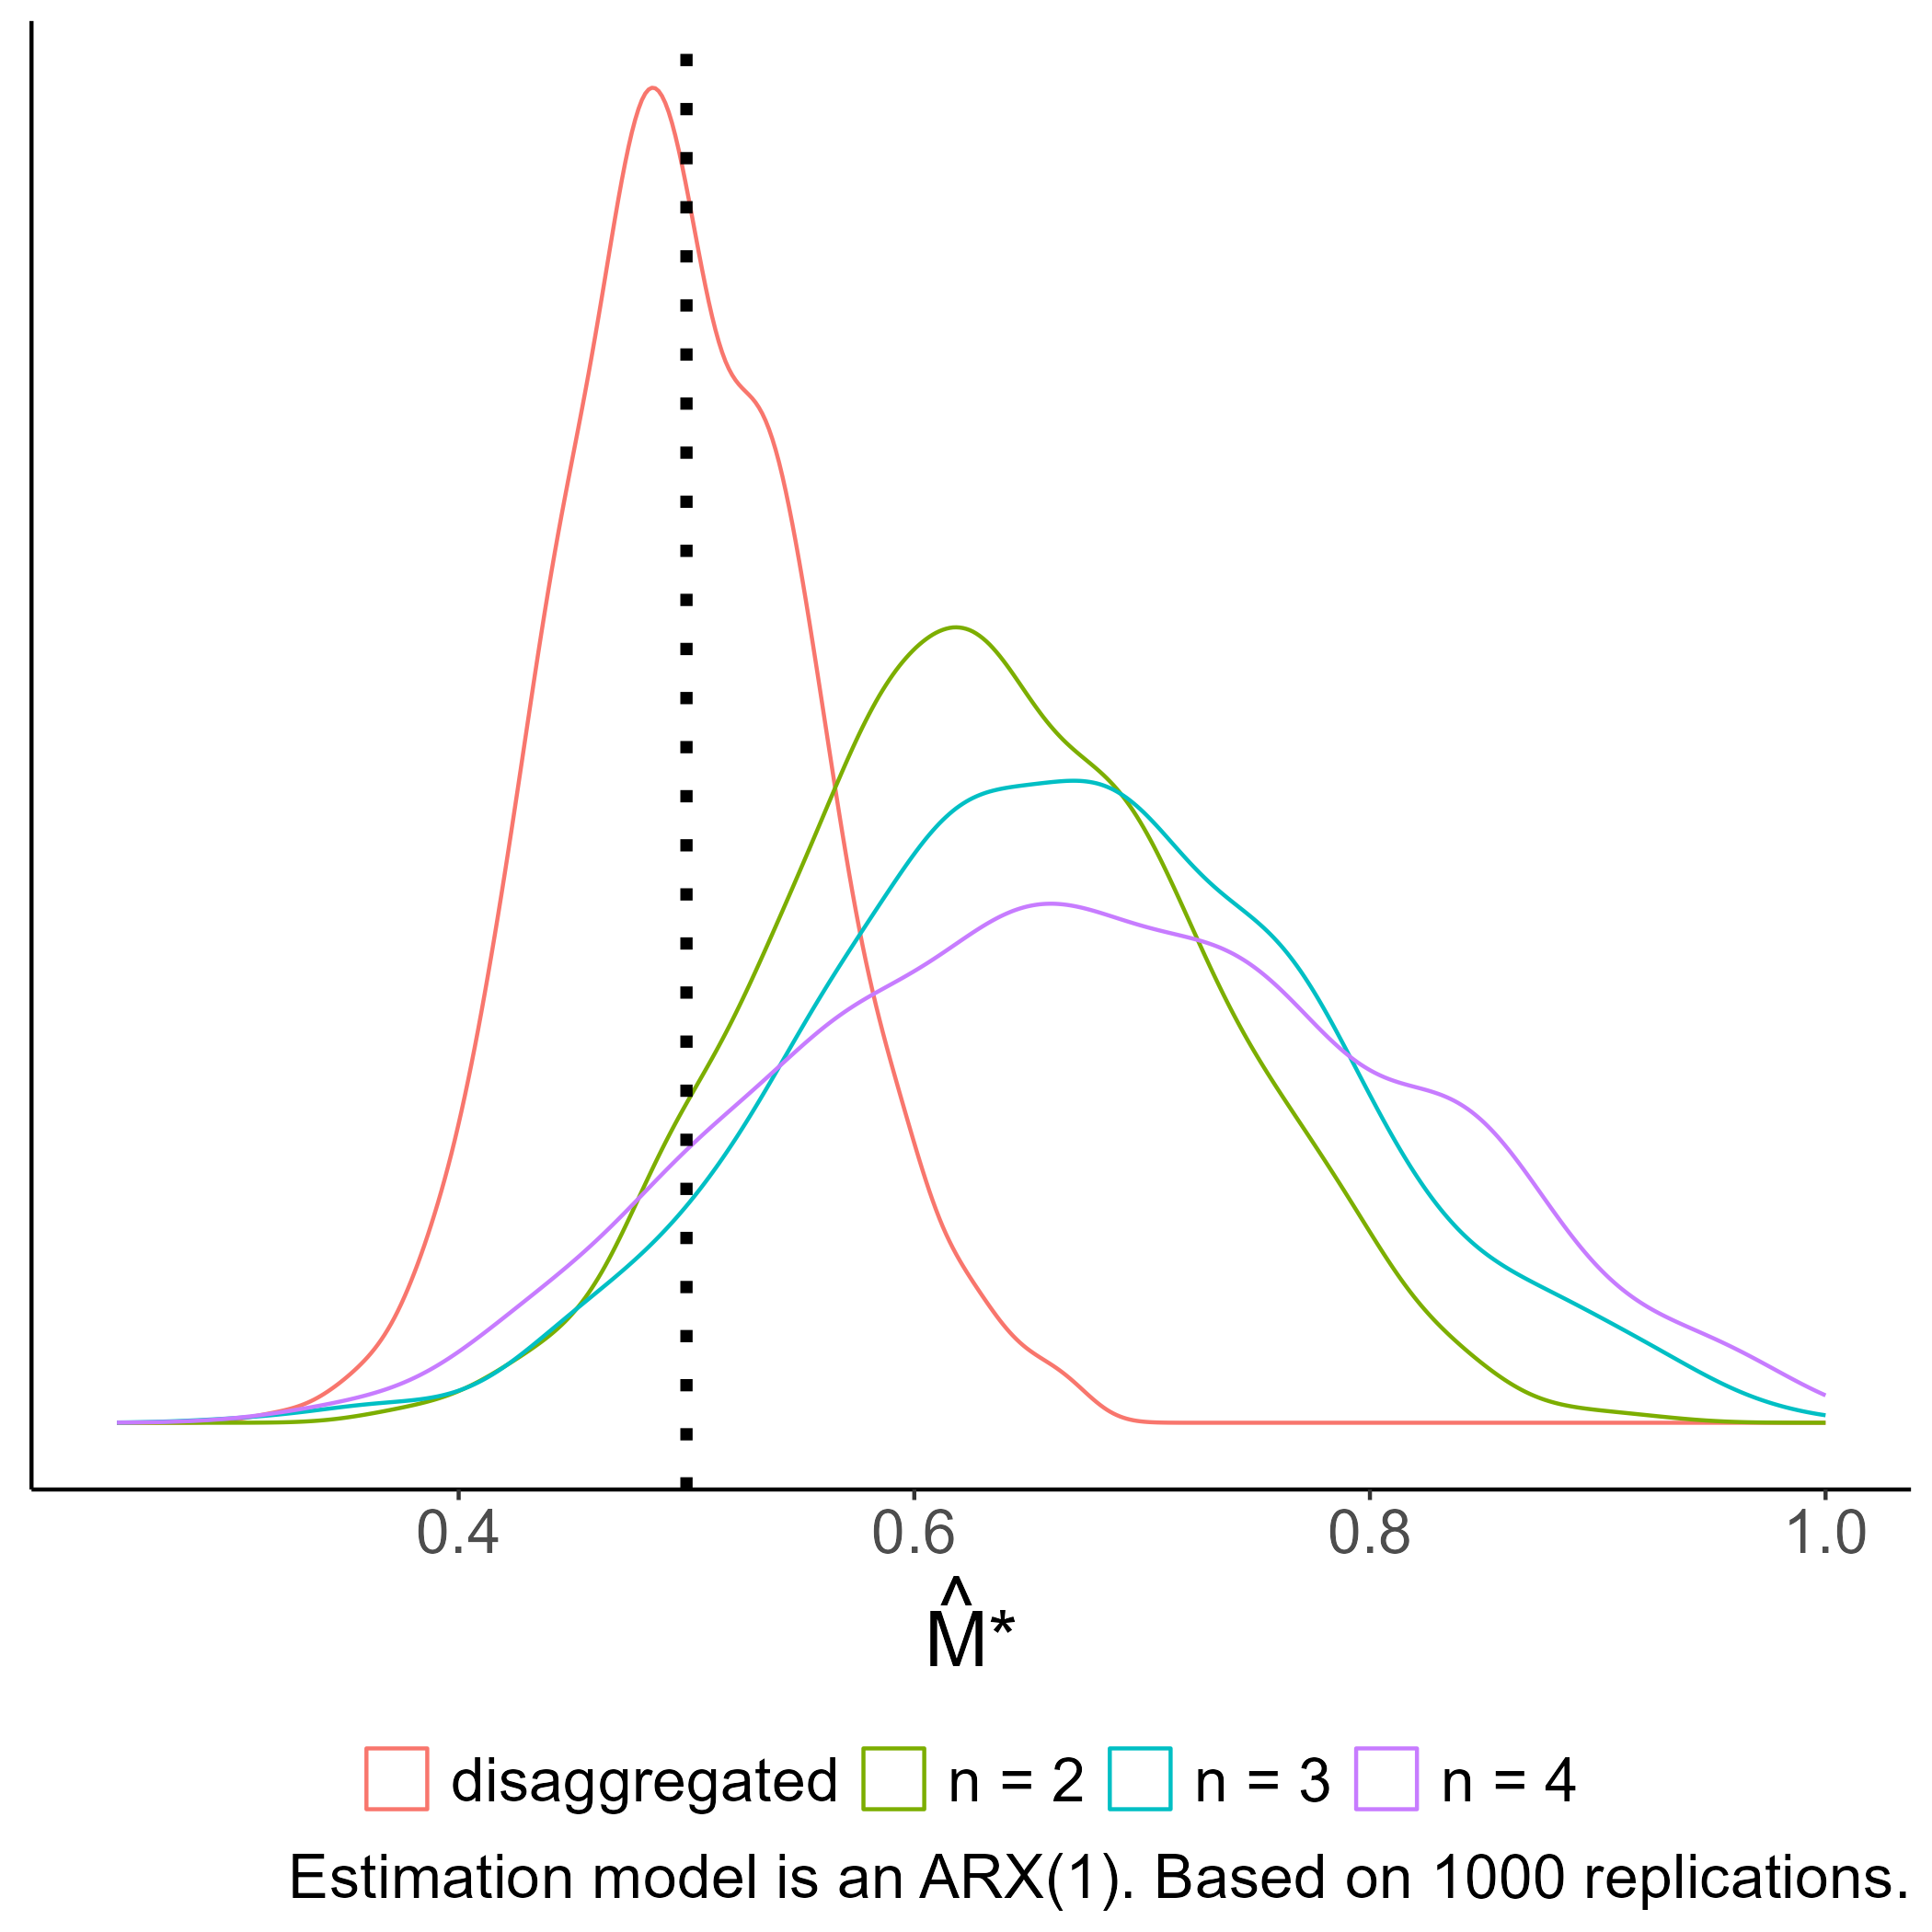
\includegraphics[width=1\linewidth]{figures/plot_MEstimates_ARX1.png}
            \end{figure}
        \end{column}
        \begin{column}{.5\textwidth}
            \begin{table}[]
                \centering
                \begin{tabular}[t]{lrrr}
                    \toprule
                     $n$    & Avg. & Bias & MC-SE \\
                     \midrule
                    1 & 0.498 & -0.002 & 0.002 \\
                    2 & 0.633 & 0.133 & 0.003\\
                    3 & 0.670 & 0.170 & 0.004\\
                    2 & 0.679 & 0.179 & 0.004\\
                    \bottomrule
                \end{tabular}
                \caption{\footnotesize{Average estimate (Avg.), bias, and Monte Carlo standard errors (MC-SE) of the bias for the effect $M$ of the time-dependent predictor, estimated using an ARX(1) model. Based on 1000 replications. $n = 1$ denotes the disaggregated data.}}
            \end{table}
        \end{column}
    \end{columns}
\end{frame}

%----

\begin{frame}{ARX(1) | Results ARMAX(1,1) model (sampling distribution $\hat{M}$)}
    \begin{columns}
        \begin{column}{.5\textwidth}
            \begin{figure}
                \centering
                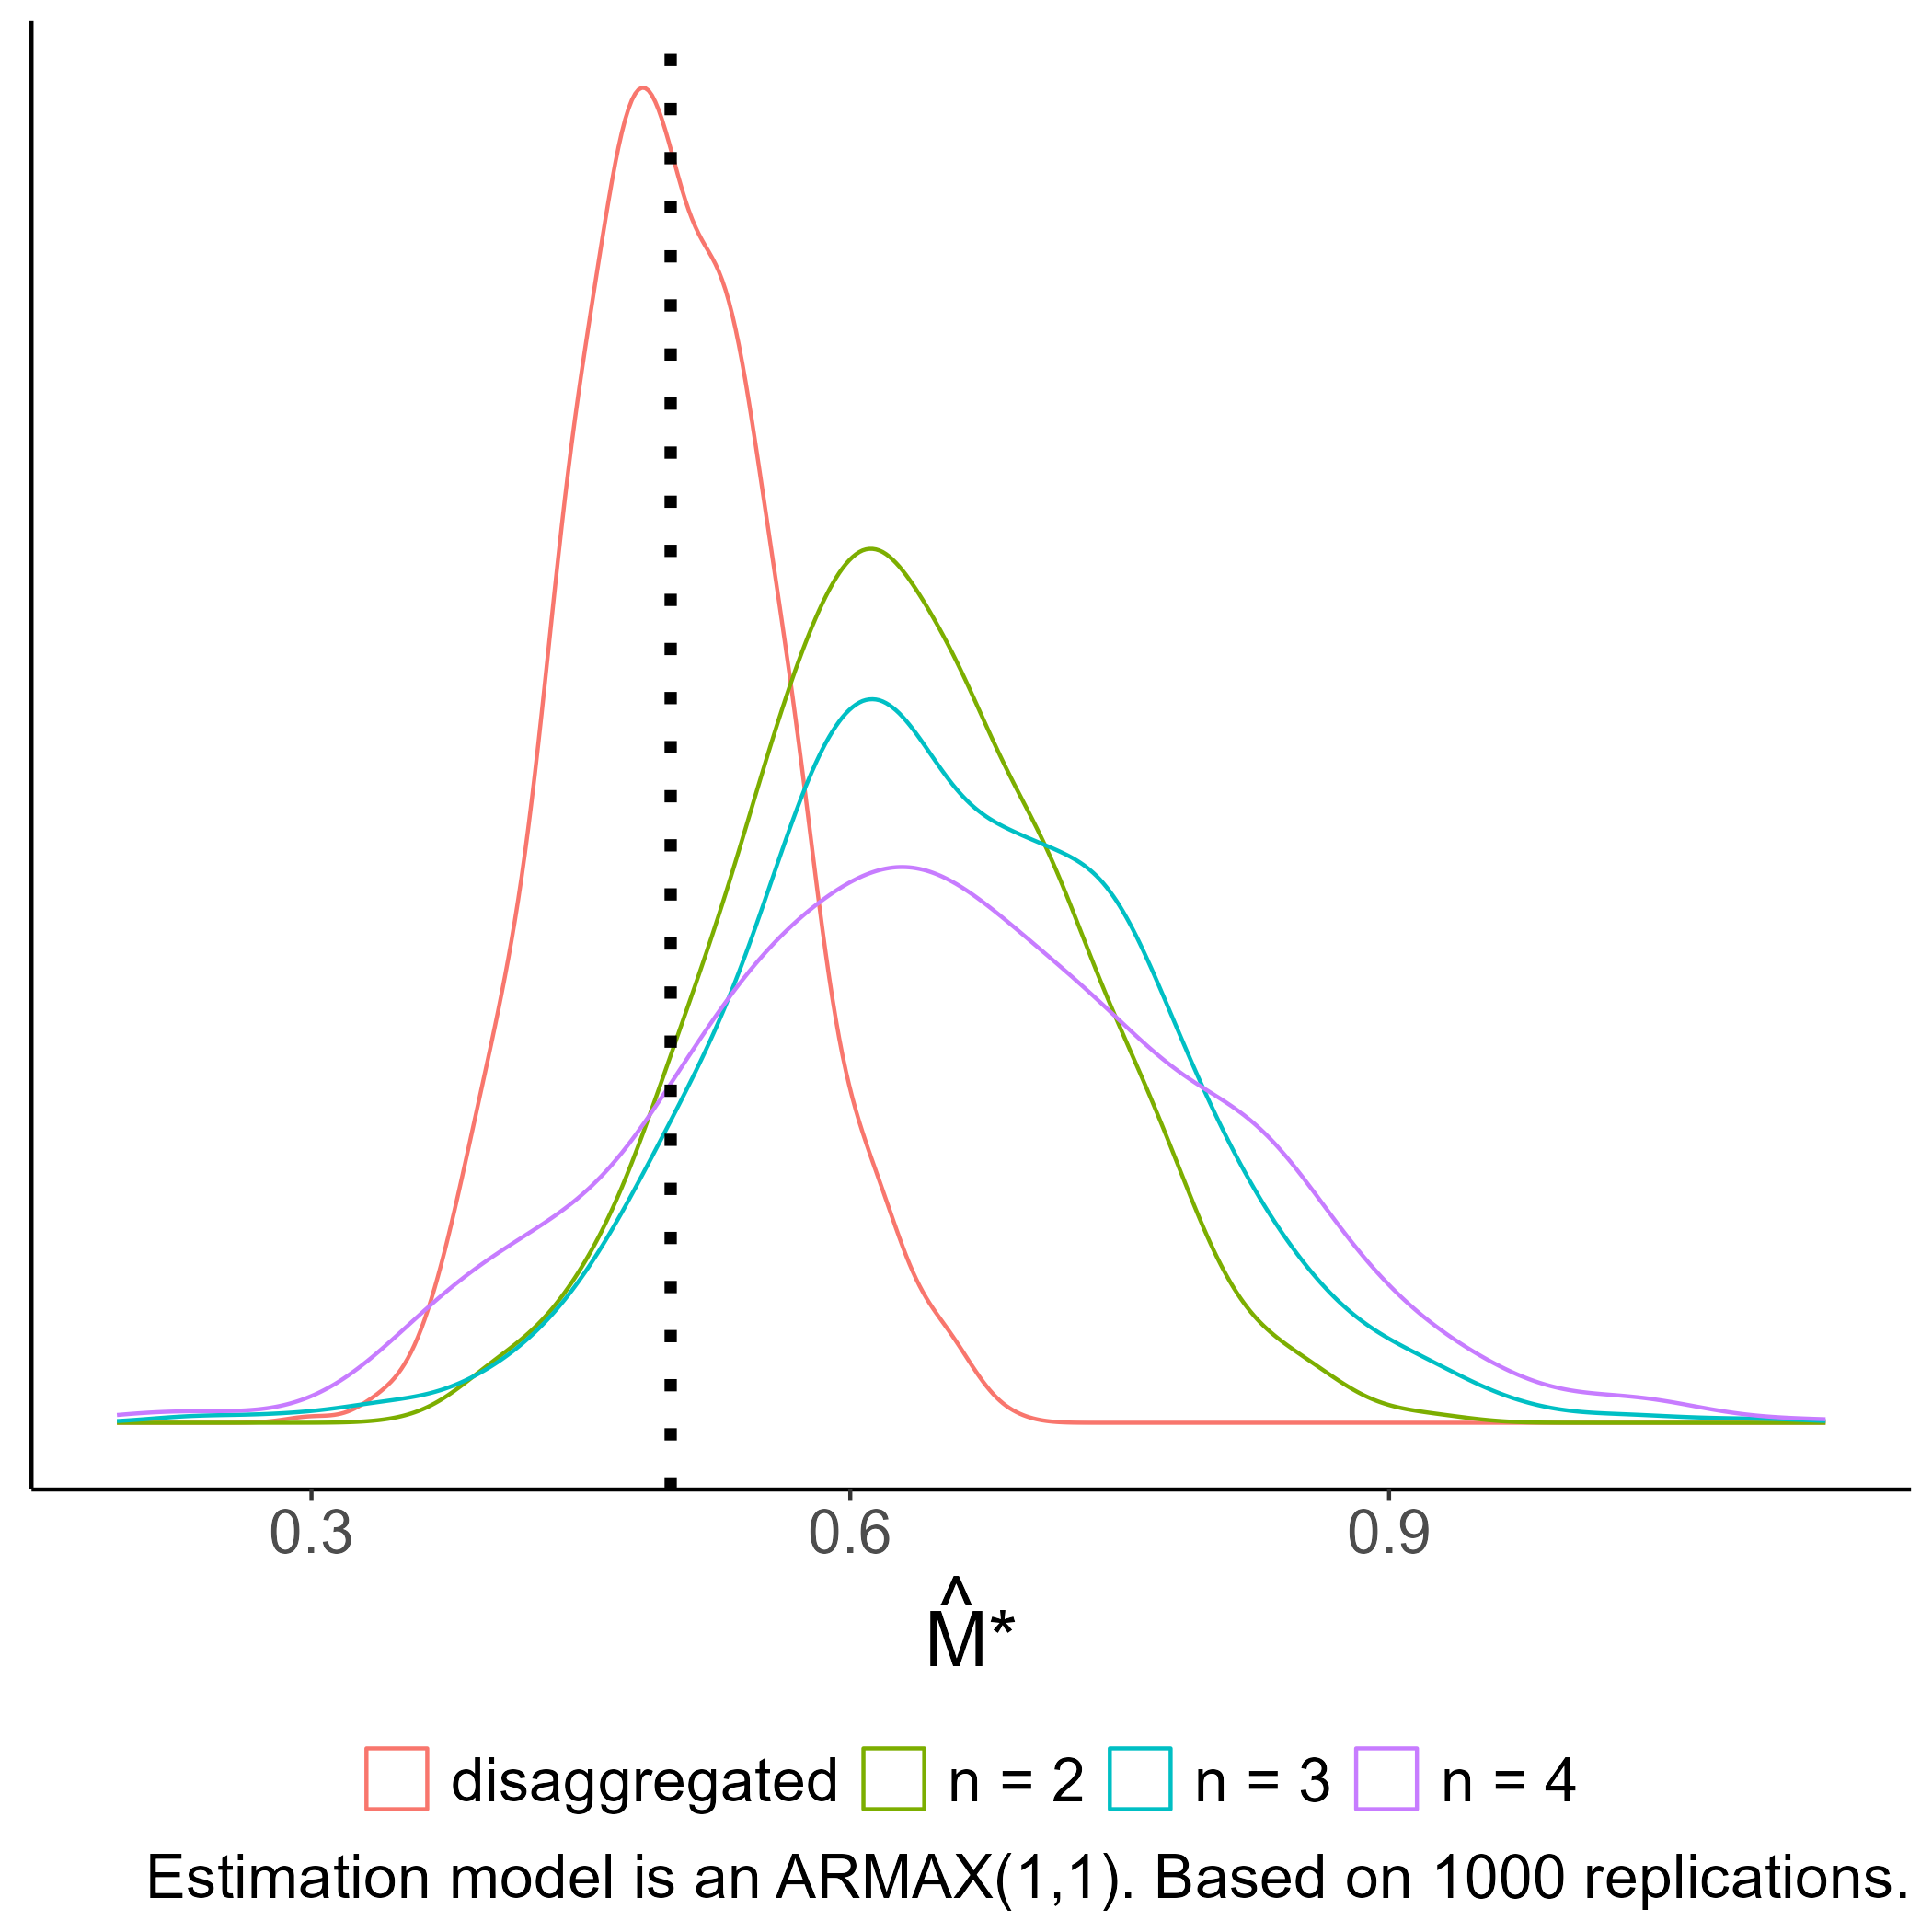
\includegraphics[width=1\linewidth]{figures/plot_MEstimates_ARMAX11.png}
            \end{figure}
        \end{column}
        \begin{column}{.5\textwidth}
            \begin{table}[]
                \centering
                \begin{tabular}[t]{lrrr}
                    \toprule
                     $n$    & Avg. & Bias & MC-SE \\
                     \midrule
                    1 & 0.500 & -0.000 & 0.002 \\
                    2 & 0.628 & 0.128 & 0.003\\
                    3 & 0.653 & 0.153 & 0.004\\
                    2 & 0.647 & 0.147 & 0.005\\
                    \bottomrule
                \end{tabular}
                \caption{\footnotesize{Average estimate (Avg.), bias, and Monte Carlo standard errors (MC-SE) of the bias for the effect $M$ of the time-dependent predictor, estimated using an ARMAX(1,1) model. Based on 1000 replications. $n = 1$ denotes the disaggregated data.}}
            \end{table}
        \end{column}
    \end{columns}
\end{frame}



%--------------------------
\subsection{Missing Frames}
%--------------------------

\begin{frame}{ARX(1) | DAG (with missing frames, every 2nd)}
    \begin{center}
        \scalebox{0.8}{
            \begin{tikzpicture}[auto, scale = 0.5,
                time/.style={rectangle, inner sep=0pt, minimum size=8mm, align=center},
                manifest/.style={rectangle,draw,very thick,inner sep=0pt,minimum width=8mm,minimum height=8mm},
                paths/.style={->, very thick, -latex},
                double/.style={very thick, -latex}
            ]
                % Nodes
                \node[manifest] (y0) at (0,0) {$Y_{0}$};
                \node[manifest, right of = y0, xshift = 2cm, text=gray, draw=gray,dotted] (y1) {$Y_{1/2}$};
                \node[manifest, right of = y1, xshift = 2cm] (y2) {$Y_{1}$};
                \node[manifest, right of = y2, xshift = 2cm, text=gray, draw=gray,dotted] (y3) {$Y_{3/2}$};
                \node[manifest, right of = y3, xshift = 2cm] (y4) {$Y_{2}$};
                
                \node[manifest, below of = y0, yshift = -1.5cm] (x0) {$\chi_{0}$};
                \node[manifest, below of = y1, yshift = -1.5cm, text=gray, draw=gray,dotted] (x1) {$\chi_{1/2}$};
                \node[manifest, below of = y2, yshift = -1.5cm] (x2) {$\chi_{1}$};
                \node[manifest, below of = y3, yshift = -1.5cm, text=gray, draw=gray,dotted] (x3) {$\chi_{3/2}$};
                \node[manifest, below of = y4, yshift = -1.5cm] (x4) {$\chi_{2}$};

                % Paths: Time-dependent effects
                \draw[paths] (x0) -- (y0);
                \draw[paths] (x1) -- (y1);
                \draw[paths] (x2) -- (y2);
                \draw[paths] (x3) -- (y3);
                \draw[paths] (x4) -- (y4);

                % Paths: Autoregressive effects
                \draw[paths] (x0) -- (x1);
                \draw[paths] (x1) -- (x2);
                \draw[paths] (x2) -- (x3);
                \draw[paths] (x3) -- (x4);
                
                \draw[paths] (y0) -- (y1);
                \draw[paths] (y1) -- (y2);
                \draw[paths] (y2) -- (y3);
                \draw[paths] (y3) -- (y4);
                
                % Time line                
                \node (timeline-start) [below of = x0, yshift = -1cm, xshift = -2cm] {};
                \node (timeline-end) [below of = x4, yshift = -1cm, xshift = 2cm] {};
            
                \draw[->, thick] (timeline-start) -- (timeline-end) node[midway, above] {};

                % Add ticks and labels for the timeline relative to the diagram nodes
                \node (t0) [below of = x0, yshift = -1.5cm] {$t_{0}$};
                \node (t1) [below of = x1, yshift = -1.5cm] {$t_{1/2}$};
                \node (t2) [below of = x2, yshift = -1.5cm] {$t_{1}$};
                \node (t3) [below of = x3, yshift = -1.5cm] {$t_{3/2}$}; 
                \node (t4) [below of = x4, yshift = -1.5cm] {$t_{2}$}; 
            
                \foreach \tick in {t0, t1, t2, t3, t4} {
                    \draw (\tick) -- ++(0,1.5); 
                }
            \end{tikzpicture}
        }
    \end{center}   
\end{frame}

%----

\begin{frame}{ARX(1) | Data file ($n = 2$)}
    \footnotesize
    \begin{table}[]
        \centering
        \begin{tabular}{ccccccc}
            \toprule
            chi & Y & t & unit & every\_2 & every\_3 & every\_4 \\
            \midrule
            1 & \textcolor{red}{0.18} & 1 & 1 & 0 & 0 & 0 \\
            1 & \textcolor{red}{-0.66} & 2 & 1 & 1 & 0 & 0 \\
            1 & \textcolor{green}{0.52} & 3 & 1 & 0 & 1 & 0 \\
            1 & \textcolor{green}{0.43} & 4 & 1 & 1 & 0 & 1 \\
            1 & \textcolor{blue}{1.41} & 5 & 1 & 0 & 0 & 0 \\
            0 & \textcolor{blue}{1.33} & 6 & 1 & 1 & 1 & 0 \\
            \bottomrule
        \end{tabular}
        \caption{First six rows of disaggregated data.}
    \end{table} \\
    \bigskip
    \begin{table}[ht]
        \centering
        \begin{tabularx}{.9\linewidth}{cccccccccc}
            \toprule
            chi & Y & t & unit & frame & chi\_mean & Y\_mean & every\_2 & every\_3 & every\_4 \\
            \midrule
            1 & -0.66 & 2 & 1 & 1 & 1.0 & \textcolor{red}{-0.24} & 0 & 0 & 0 \\
            1 & 0.43 & 4 & 1 & 2 & 1.0 & \textcolor{green}{0.48} & 1 & 0 & 0 \\
            0 & 1.33 & 6 & 1 & 3 & 0.5 & \textcolor{blue}{1.37} & 0 & 1 & 0 \\
            \bottomrule
        \end{tabularx}
        \caption{Corresponding aggregated data ($n = 2$).}
    \end{table}
\end{frame}

%----

\begin{frame}{ARX(1) | Mplus syntax (every 2nd)}
    \begin{table}
        \setlength\extrarowheight{2pt}
        \begin{center}
            \scalebox{0.7}{
                \begin{tabular}{ p{2.8cm} p{9.8cm} }
                \hline
                \\[-2.3mm]
                    \textcolor{blue}{VARIABLE:} & NAMES = chi Y t Unit frame chiAggr yAggr every\_2 every\_3 every\_4;\\
                     & USEOBSERVATIONS = (every\_2 EQ 1);\\
                     & USEVARIABLES = chiAggr yAggr;\\
                     & LAGGED = yAggr(1);\\
                    \\
                    \textcolor{blue}{ANALYSIS:} & PROCESSOR = 4;\\
                                                & ESTIMATOR = BAYES;\\
                                                & BITERATION = (1000);
                                                & \\
                    \textcolor{blue}{MODEL:}    & yAggr ON 0.5*yAggr\&1 0.5*chiAggr;\\
                \\[-2.3mm]
                \hline
                \end{tabular}
            }
        \end{center}
    \end{table}
\end{frame}

%----

\begin{frame}{ARX(1) | Results ARX(1) with missing frames (sampling distribution $\hat{A}$)}
    \begin{figure}
        \centering
        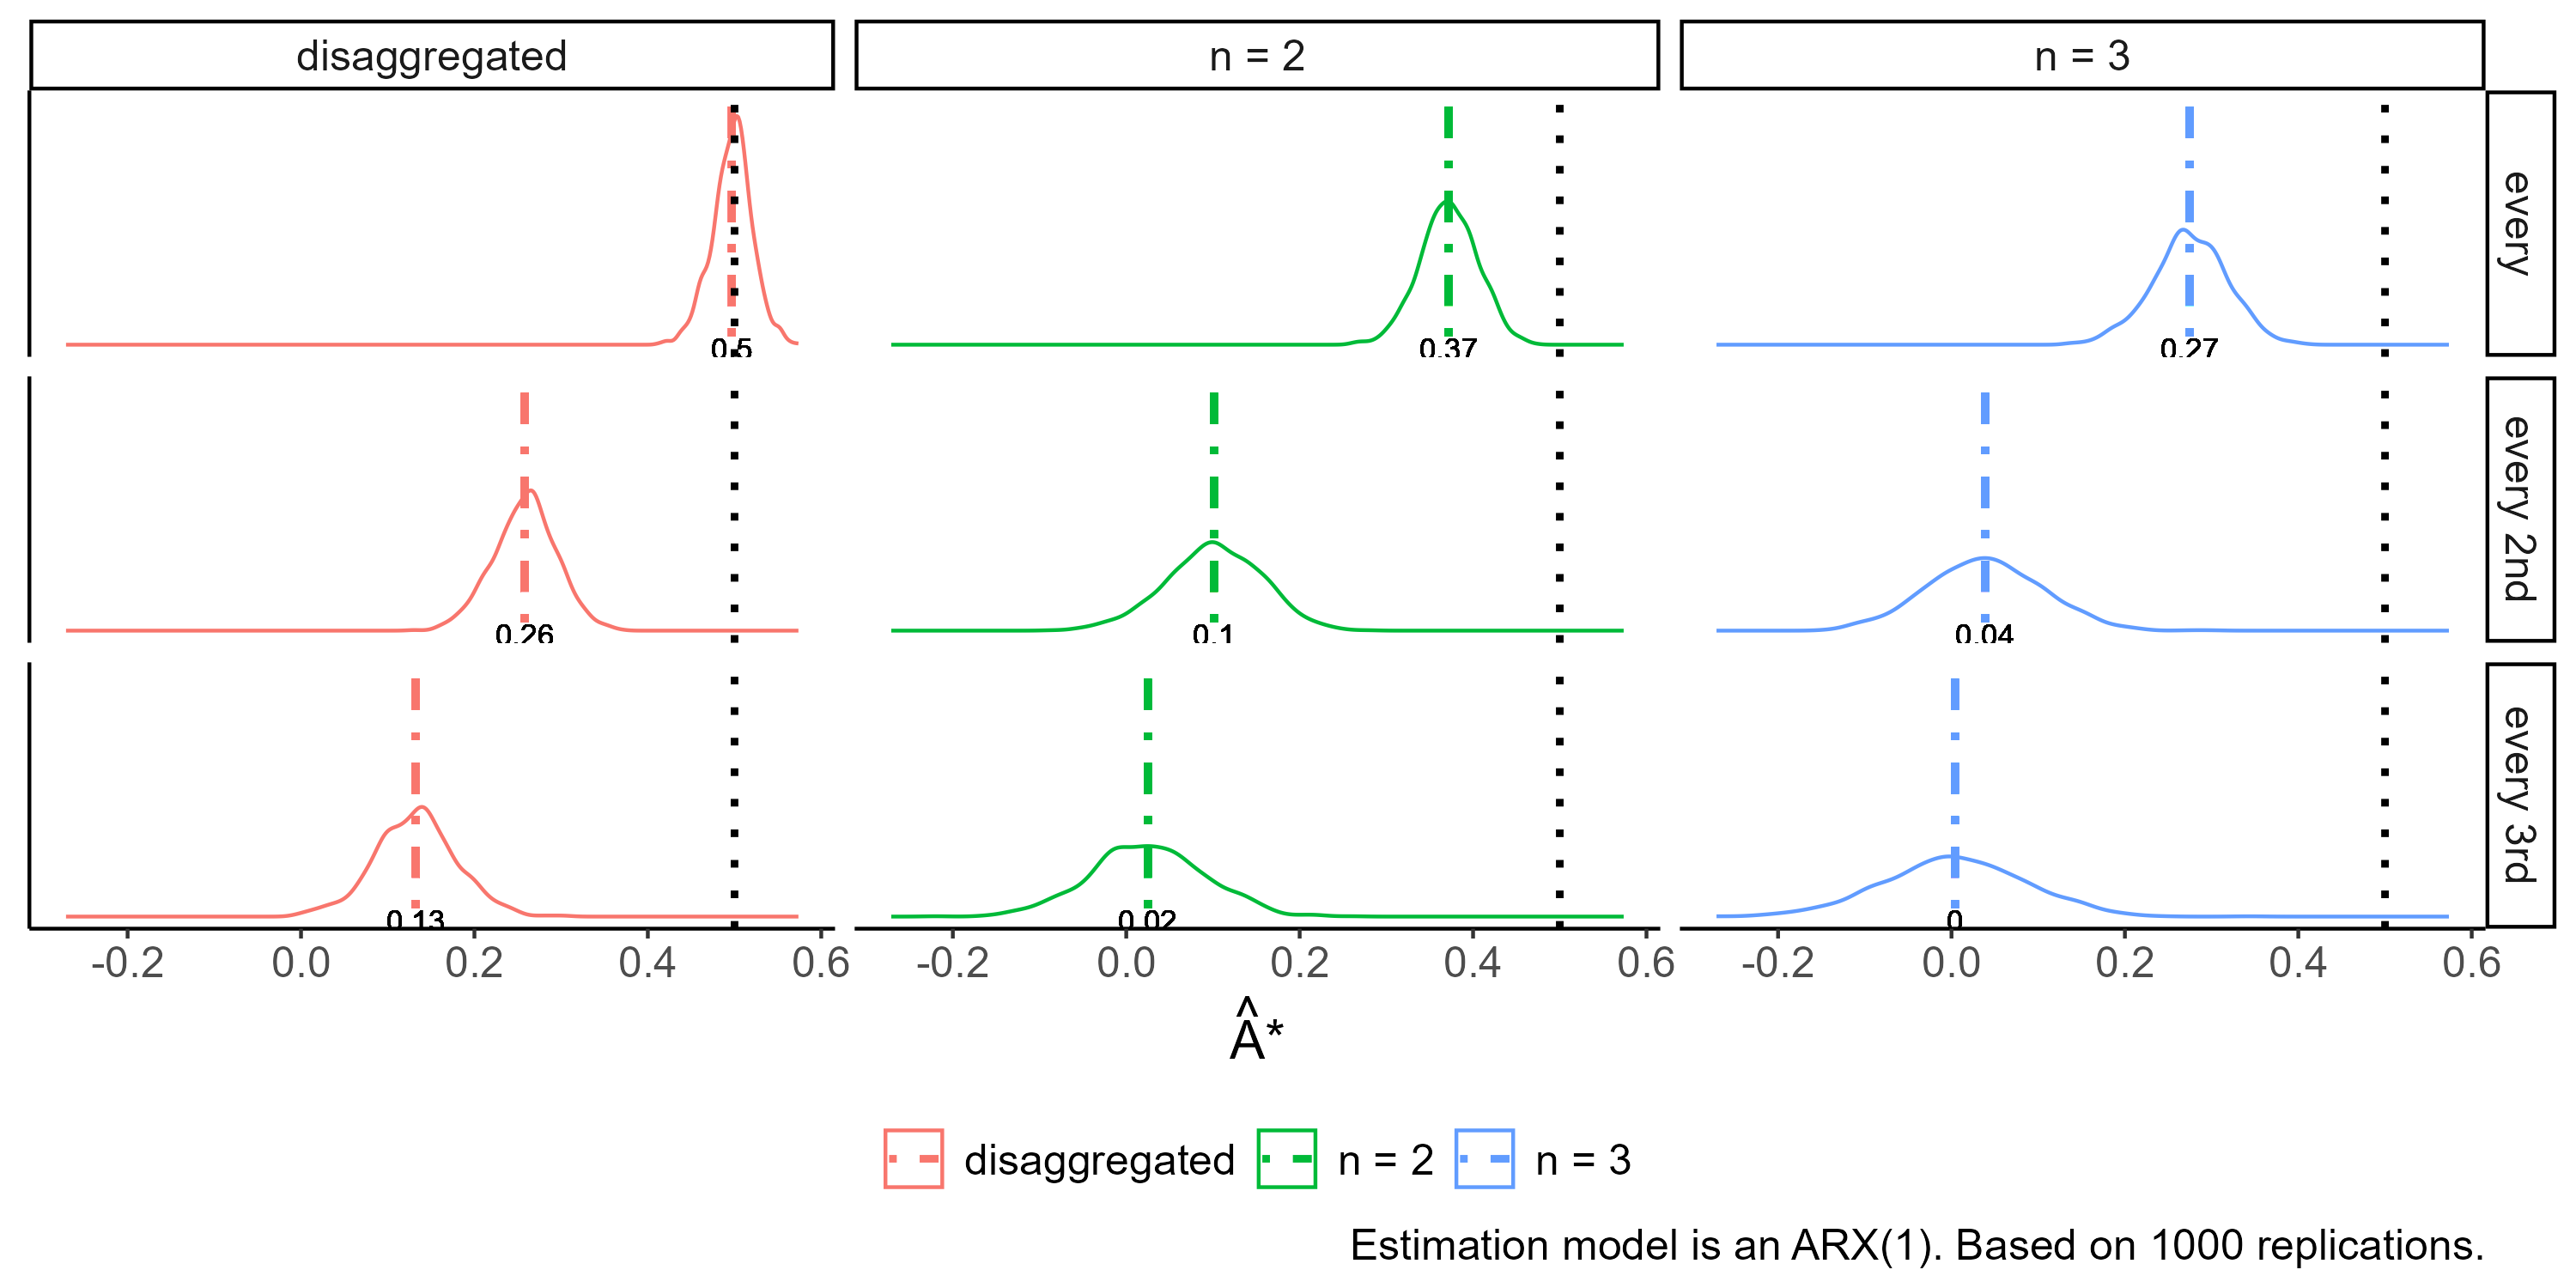
\includegraphics[width=1\linewidth]{figures/plot_AEstimates_ARX1_missing.png}
    \end{figure}
\end{frame}

%-----

\begin{frame}{ARX(1) | Results ARX(1) with missing frames (sampling distribution $\hat{M}$)}
    \begin{figure}
        \centering
        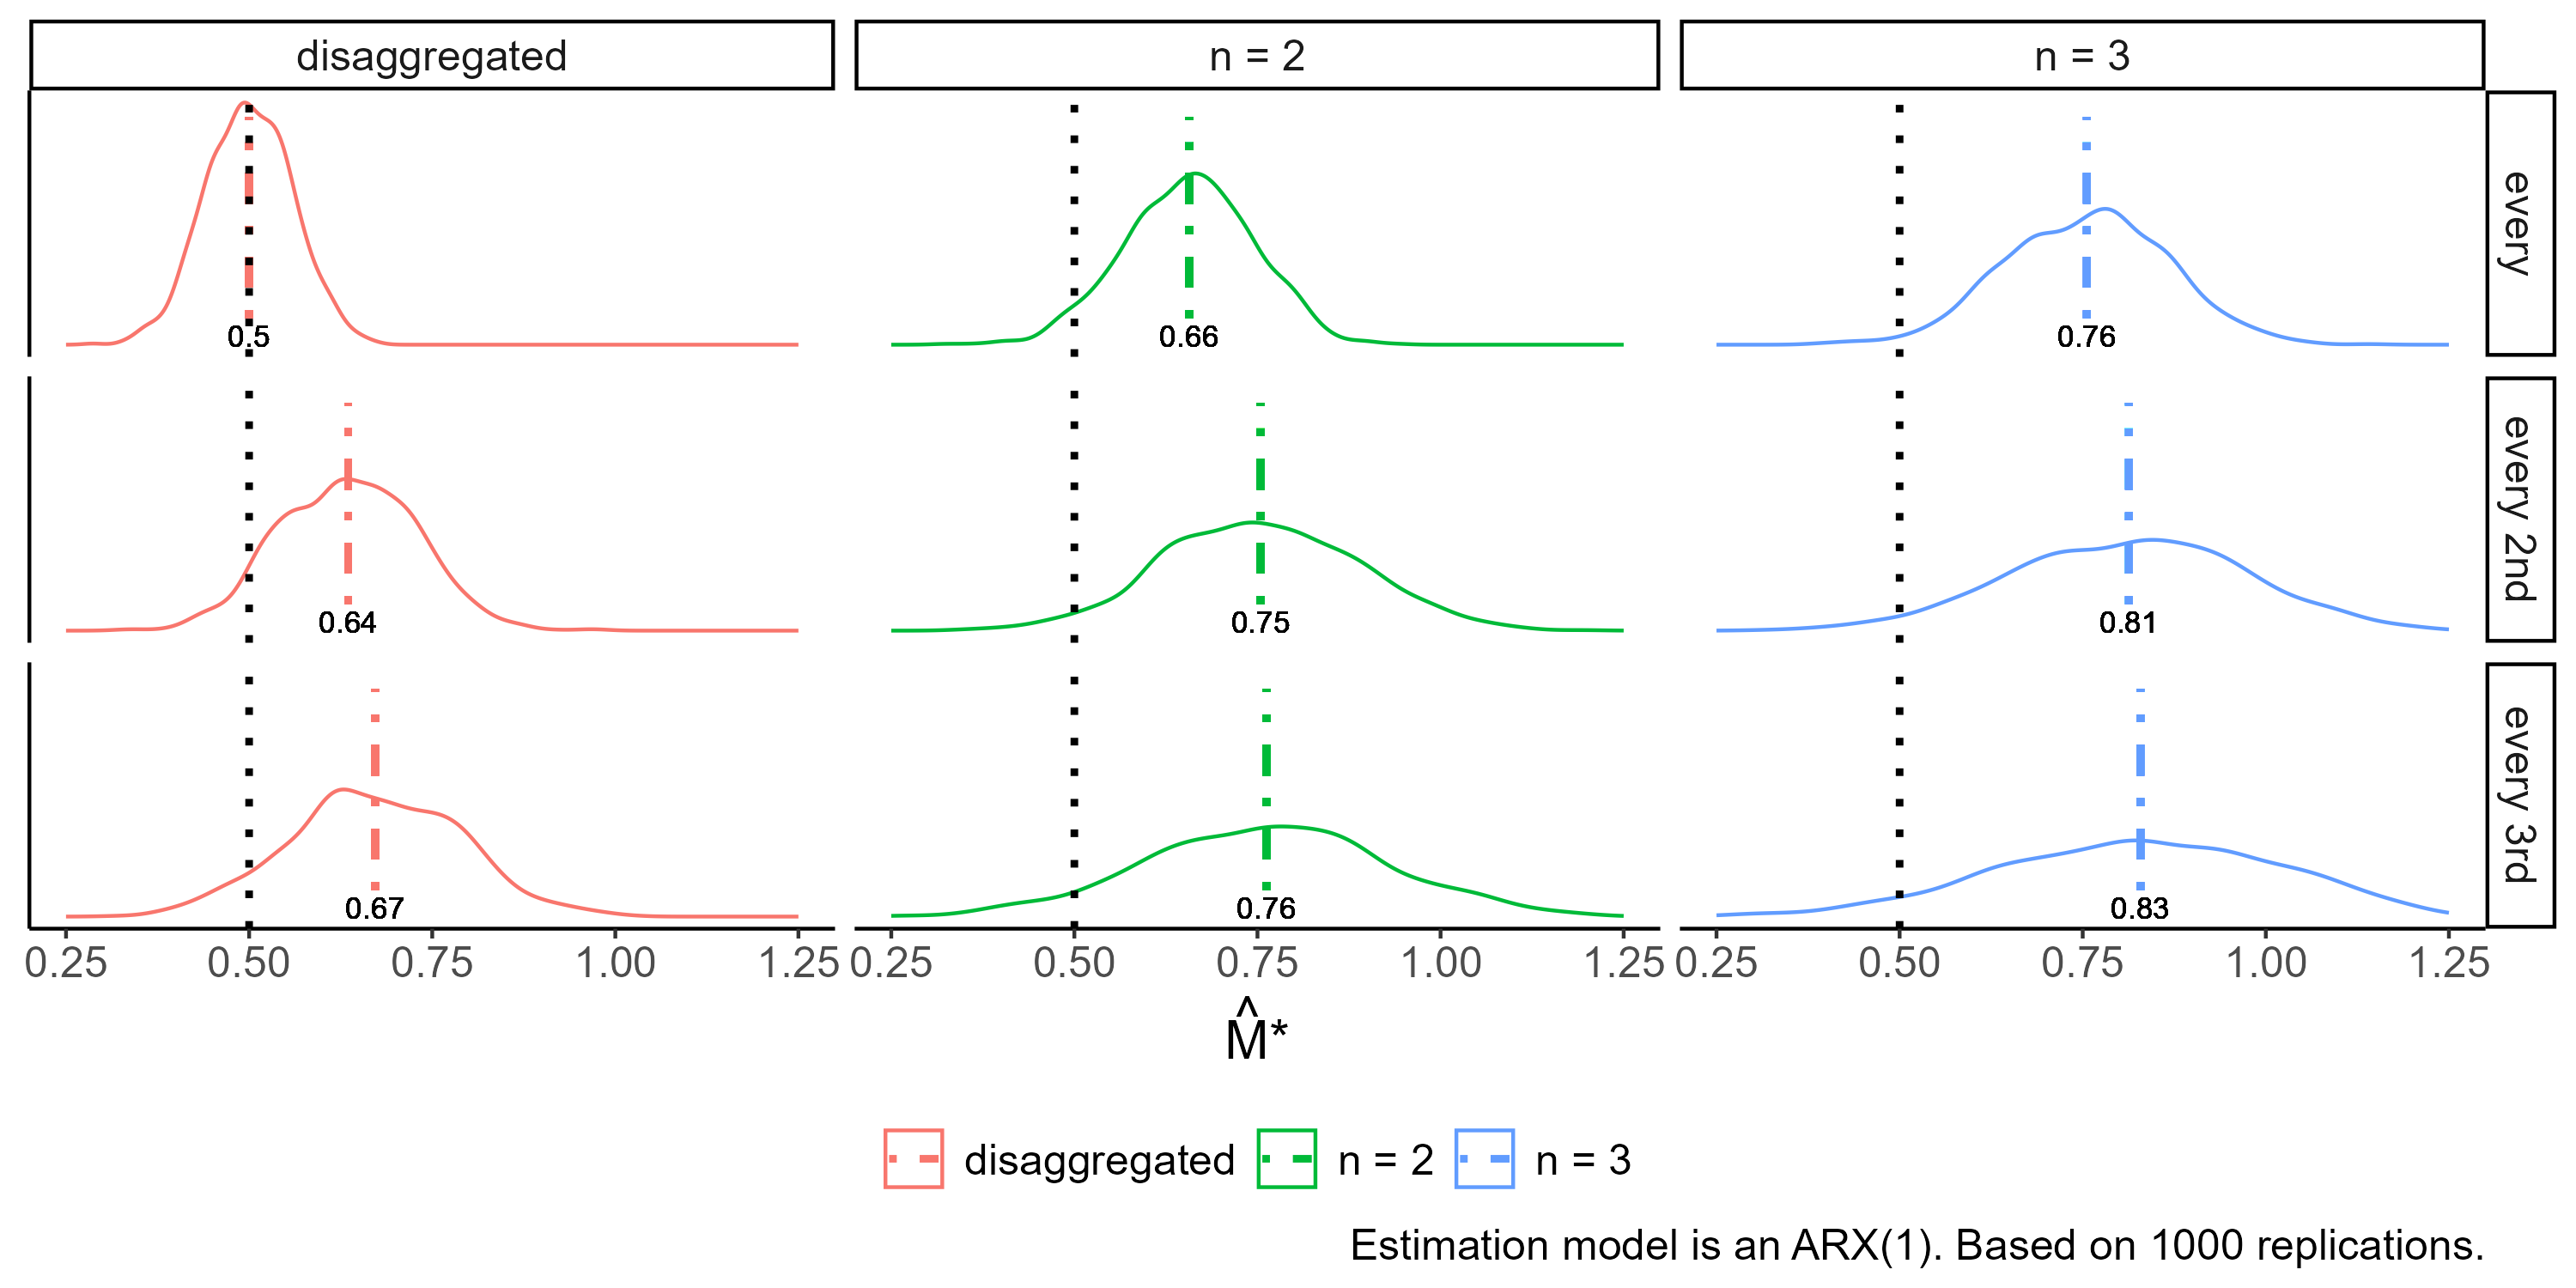
\includegraphics[width=1\linewidth]{figures/plot_MEstimates_ARX1_missing.png}
    \end{figure}
\end{frame}

%--------------------------------
\subsection{Measurement Error}
%--------------------------------

\begin{frame}{MEARX(1) | Analysis by MEARX(1)}
    Mplus syntax for ME-ARX(1) model:
    \begin{table}
        \setlength\extrarowheight{2pt}
        \begin{center}
            \scalebox{0.7}{
                \begin{tabular}{ p{2.8cm} p{9.8cm} }
                \hline
                \\[-2.3mm]
                    \textcolor{blue}{ANALYSIS:} & PROCESSOR = 4;\\
                                                & ESTIMATOR = BAYES;\\
                                                & BITERATION = (1000);
                                                & \\
                    \textcolor{blue}{MODEL:}    & \textcolor{green}{! Measurement model}\\
                                                & eta BY y@1 (\&1); \\
                                                & y; \textcolor{green}{! Measurement error}\\
                                                & \\
                                                & eta ON 0.5*eta\&1 0.5*chi;\\
                                                & eta; \textcolor{green}{! Residual error}\\
                \\[-2.3mm]
                \hline
                \end{tabular}
            }
        \end{center}
    \end{table}
\end{frame}

%----

\begin{frame}{MEARX(1) | Results MEARX(1)}
    Convergence is slow, hence I only display results for $n = 1, 2$ and an indicator reliability of 0.8: 
    \bigskip
    \begin{table}[]
        \centering
        \begin{tabular}{ccccccccc}
            \toprule
                & & \multicolumn{3}{c}{disaggregated} & & \multicolumn{3}{c}{$n = 2$}\\ 
            \cmidrule{3-5} \cmidrule{7-9} 
            Parameter & Pop. & Avg. & Std. Dev. & S.E. Avg. & & Avg. & Std. Dev. & S.E. Avg. \\
            \midrule
            $\hat{A}$ & 0.5 & 0.514 & 0.030 & 0.035 & & 0.389 & 0.035 & 0.044 \\
            $\hat{M}$ & 0.5 & 0.493 & 0.050 & 0.050 & & 0.651 & 0.072 & 0.072 \\
            \bottomrule
        \end{tabular}
        \caption{Based on 1000 replications.}
    \end{table}
\end{frame}

%----

\begin{frame}{MEARX(1) | Results ARX(1) by reliability (sampling distribution $\hat{A}$)}
    \begin{figure}
        \centering
        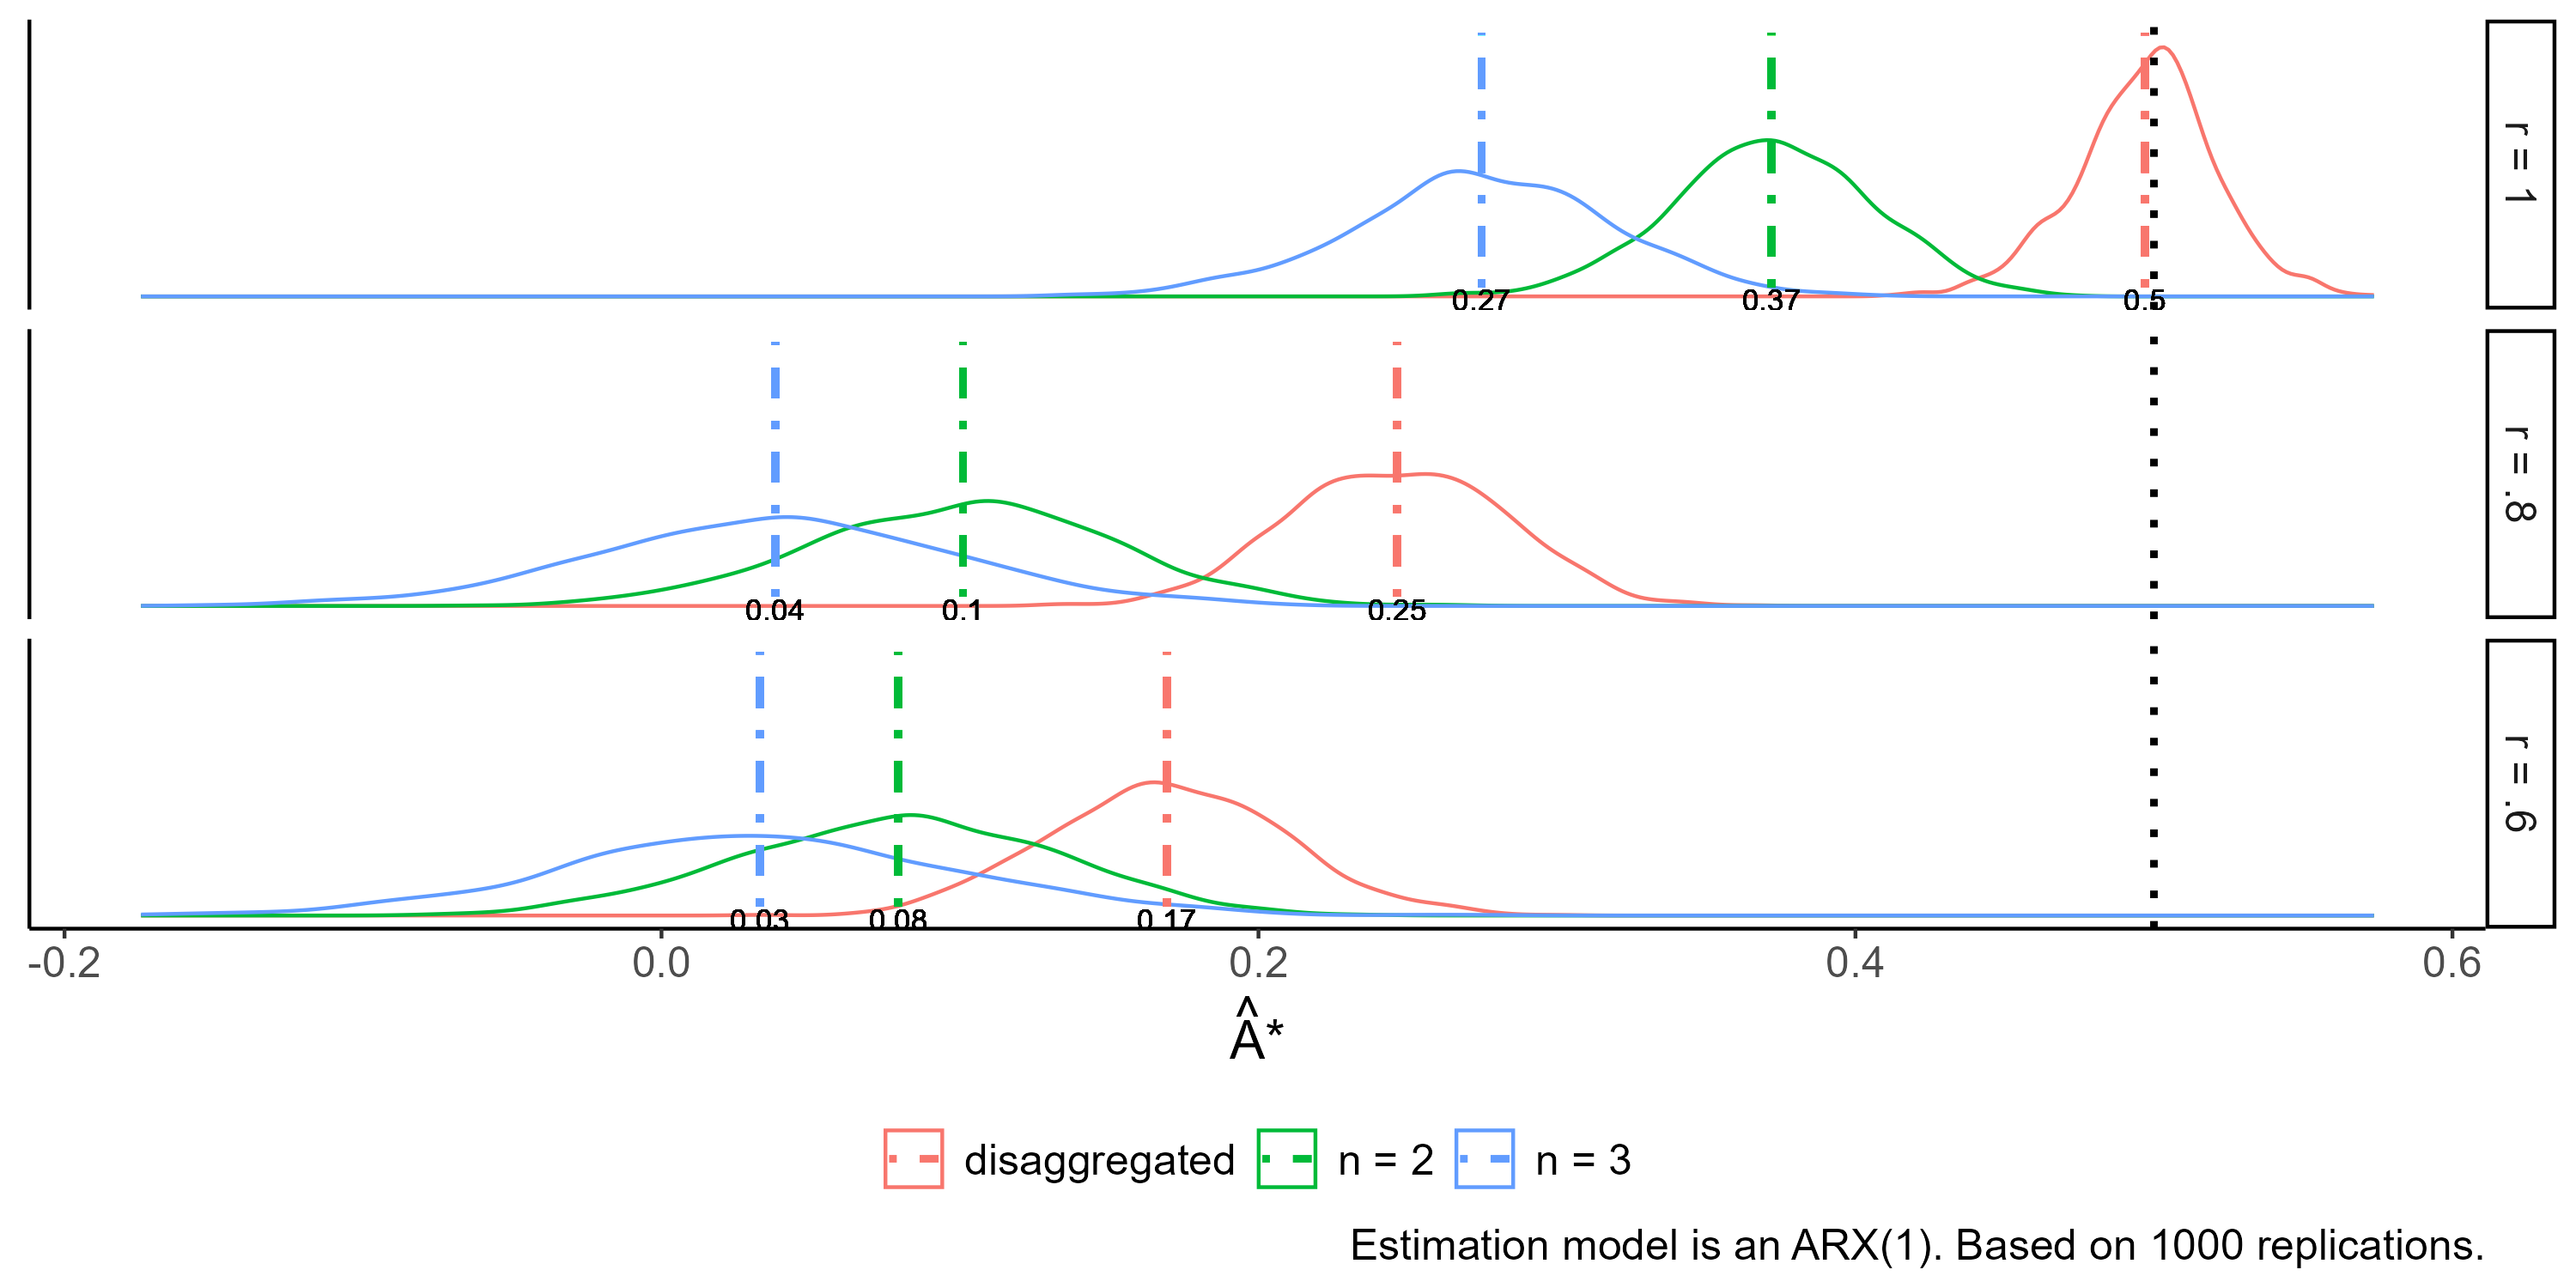
\includegraphics[width=1\linewidth]{figures/plot_AEstimates_ARX1_rel.png}
    \end{figure}
\end{frame}

%----

\begin{frame}{MEARX(1) | Results ARX(1) by reliability (sampling distribution $\hat{M}$)}
    \begin{figure}
        \centering
        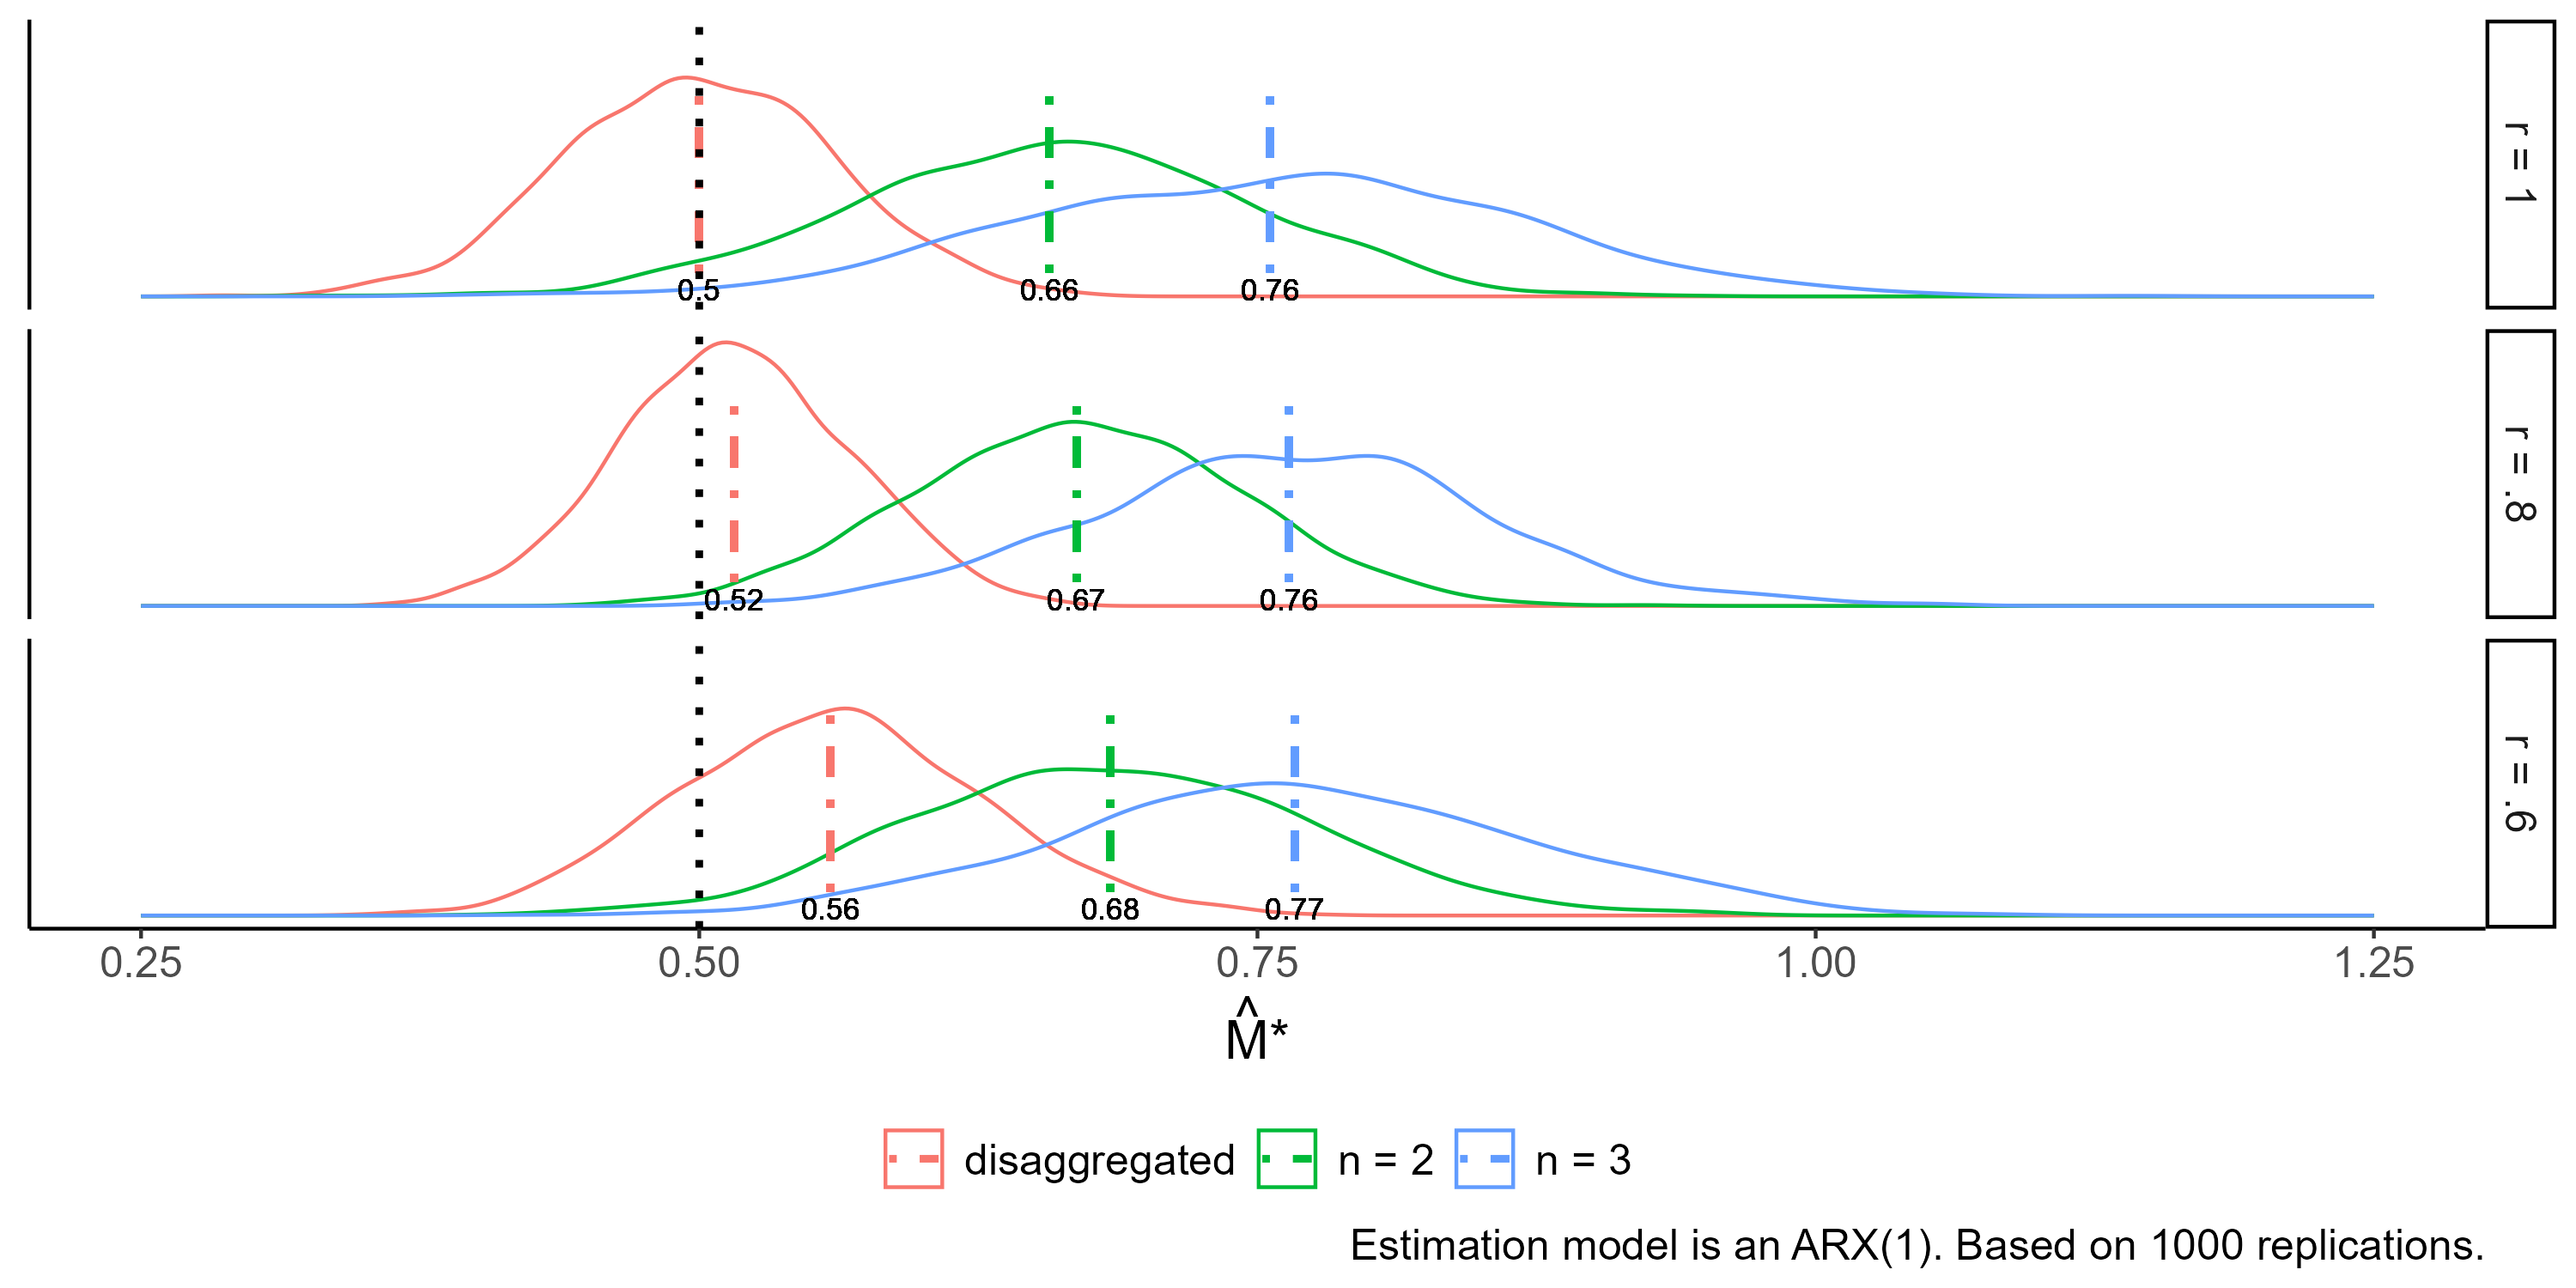
\includegraphics[width=1\linewidth]{figures/plot_MEstimates_ARX1_rel.png}
    \end{figure}    
\end{frame}

%--------------------------------
\subsection{Including Covariates}
%--------------------------------

\begin{frame}{VAR(1) | DAG (with missing frames, every 2nd) I}
    \begin{center}
        \scalebox{0.7}{
            \begin{tikzpicture}[auto, scale = 0.5,
                time/.style={rectangle, inner sep=0pt, minimum size=8mm, align=center},
                manifest/.style={rectangle,draw,very thick,inner sep=0pt,minimum width=8mm,minimum height=8mm},
                paths/.style={->, very thick, -latex},
                double/.style={very thick, -latex}
            ]
                % Nodes
                \node[manifest] (y0) at (0,0) {$Y_{0}$};
                \node[manifest, right of = y0, xshift = 2cm, text=gray, draw=gray,dotted] (y1) {$Y_{1/2}$};
                \node[manifest, right of = y1, xshift = 2cm] (y2) {$Y_{1}$};
                \node[manifest, right of = y2, xshift = 2cm, text=gray, draw=gray,dotted] (y3) {$Y_{3/2}$};
                \node[manifest, right of = y3, xshift = 2cm] (y4) {$Y_{2}$};
                
                \node[manifest, below of = y0, yshift = -1.5cm] (x0) {$\chi_{0}$};
                \node[manifest, below of = y1, yshift = -1.5cm, text=gray, draw=gray,dotted] (x1) {$\chi_{1/2}$};
                \node[manifest, below of = y2, yshift = -1.5cm] (x2) {$\chi_{1}$};
                \node[manifest, below of = y3, yshift = -1.5cm, text=gray, draw=gray,dotted] (x3) {$\chi_{3/2}$};
                \node[manifest, below of = y4, yshift = -1.5cm] (x4) {$\chi_{2}$};

                \node[manifest, below of = x0, yshift = -1.5cm] (l0) {$L_{0}$};
                \node[manifest, below of = x1, yshift = -1.5cm, text=gray, draw=gray,dotted] (l1) {$L_{1/2}$};
                \node[manifest, below of = x2, yshift = -1.5cm] (l2) {$L_{1}$};
                \node[manifest, below of = x3, yshift = -1.5cm, text=gray, draw=gray,dotted] (l3) {$L_{3/2}$};
                \node[manifest, below of = x4, yshift = -1.5cm] (l4) {$L_{2}$};

                % Paths: Time-dependent effects
                \draw[paths] (x0) -- (y0);
                \draw[paths] (x1) -- (y1);
                \draw[paths] (x2) -- (y2);
                \draw[paths] (x3) -- (y3);
                \draw[paths] (x4) -- (y4);

                \draw[paths] (l0) -- (x0);
                \draw[paths] (l1) -- (x1);
                \draw[paths] (l2) -- (x2);
                \draw[paths] (l3) -- (x3);
                \draw[paths] (l4) -- (x4);
                
                \draw[paths] (l0) -- (x0);
                \draw[paths] (l1) -- (x1);
                \draw[paths] (l2) -- (x2);
                \draw[paths] (l3) -- (x3);
                \draw[paths] (l4) -- (x4);

                \draw[double](l0.north west) to [out=135, in=225] (y0.south west);
                \draw[double](l1.north west) to [out=135, in=225] (y1.south west);
                \draw[double](l2.north west) to [out=135, in=225] (y2.south west);
                \draw[double](l3.north west) to [out=135, in=225] (y3.south west);
                \draw[double](l4.north west) to [out=135, in=225] (y4.south west);

                % Paths: Lag-1 effects
                \draw[paths] (y0.south east) -- (x1.north west);
                \draw[paths] (y1.south east) -- (x2.north west);
                \draw[paths] (y2.south east) -- (x3.north west);
                \draw[paths] (y3.south east) -- (x4.north west);

                % Paths: Autoregressive effects
                \draw[paths] (x0) -- (x1);
                \draw[paths] (x1) -- (x2);
                \draw[paths] (x2) -- (x3);
                \draw[paths] (x3) -- (x4);
                
                \draw[paths] (y0) -- (y1);
                \draw[paths] (y1) -- (y2);
                \draw[paths] (y2) -- (y3);
                \draw[paths] (y3) -- (y4);

                \draw[paths] (l0) -- (l1);
                \draw[paths] (l1) -- (l2);
                \draw[paths] (l2) -- (l3);
                \draw[paths] (l3) -- (l4);
                
                % Time line                
                \node (timeline-start) [below of = l0, yshift = -1cm, xshift = -2cm] {};
                \node (timeline-end) [below of = l4, yshift = -1cm, xshift = 2cm] {};
            
                \draw[->, thick] (timeline-start) -- (timeline-end) node[midway, above] {};

                % Add ticks and labels for the timeline relative to the diagram nodes
                \node (t0) [below of = l0, yshift = -1.5cm] {$t_{0}$};
                \node (t1) [below of = l1, yshift = -1.5cm] {$t_{1/2}$};
                \node (t2) [below of = l2, yshift = -1.5cm] {$t_{1}$};
                \node (t3) [below of = l3, yshift = -1.5cm] {$t_{3/2}$}; 
                \node (t4) [below of = l4, yshift = -1.5cm] {$t_{2}$}; 
            
                \foreach \tick in {t0, t1, t2, t3, t4} {
                    \draw (\tick) -- ++(0,1.5); 
                }
            \end{tikzpicture}
        }
    \end{center}   
\end{frame}

%----

\begin{frame}{VAR(1) | DAG (with missing frames, every 2nd) II}
    \textbf{Open backdoor paths $\chi_{1} \rightarrow Y_{1}$:}
    \begin{itemize}
        \item $\chi_{1} \leftarrow \chi_{1/2} \rightarrow Y_{1/2} \righarrow Y_{1}$
        \item $\chi_{1} \leftarrow \chi_{1/2} \leftarrow L_{1/2} \rightarrow Y_{1/2} \rightarrow Y_{1}$
        \item $\chi_{1} \leftarrow Y_{1/2} \rightarrow Y_{1}$
    \end{itemize}
    \bigskip
    \textbf{Open backdoor paths $L_{1} \rightarrow Y_{1}$:}
    \begin{itemize}
        \item $L_{1} \leftarrow L_{1/2} \rightarrow \chi_{1/2} \rightarrow Y_{1/2} \rightarrow Y_{1}$
        \item $L_{1} \leftarrow L_{1/2} \rightarrow Y_{1/2} \rightarrow Y_{1}$
        \item $L_{1} \leftarrow L_{1/2} \rightarrow \chi_{1/2} \rightarrow \chi_{1} \leftarrow Y_{1/2} \rightarrow Y_{1}$
    \end{itemize}
\end{frame}

%----

\begin{frame}{VAR(1) | Mplus syntax (adjustment for $L$, every 2nd)}
    \begin{table}
        \setlength\extrarowheight{2pt}
        \begin{center}
            \scalebox{0.7}{
                \begin{tabular}{ p{2.8cm} p{9.8cm} }
                \hline
                \\[-2.3mm]
                    \textcolor{blue}{VARIABLE:} & NAMES = chi Y t Unit frame chiAggr yAggr every\_2 every\_3 every\_4;\\
                     & USEOBSERVATIONS = (every\_2 EQ 1);\\
                     & USEVARIABLES = chiAggr yAggr;\\
                     & LAGGED = yAggr(1);\\
                    \\
                    \textcolor{blue}{ANALYSIS:} & PROCESSOR = 4;\\
                                                & ESTIMATOR = BAYES;\\
                                                & BITERATION = (1000);
                                                & \\
                    \textcolor{blue}{MODEL:}    & yAggr ON 0.5*yAggr\&1 0.5*chiAggr 0.8*1;\\
                \\[-2.3mm]
                \hline
                \end{tabular}
            }
        \end{center}
    \end{table}
\end{frame}

%----

\begin{frame}{VAR(1) | Results ARX(1) (adjustment for $L$, sampling distribution $\hat{A}$)}
    \begin{figure}
        \centering
        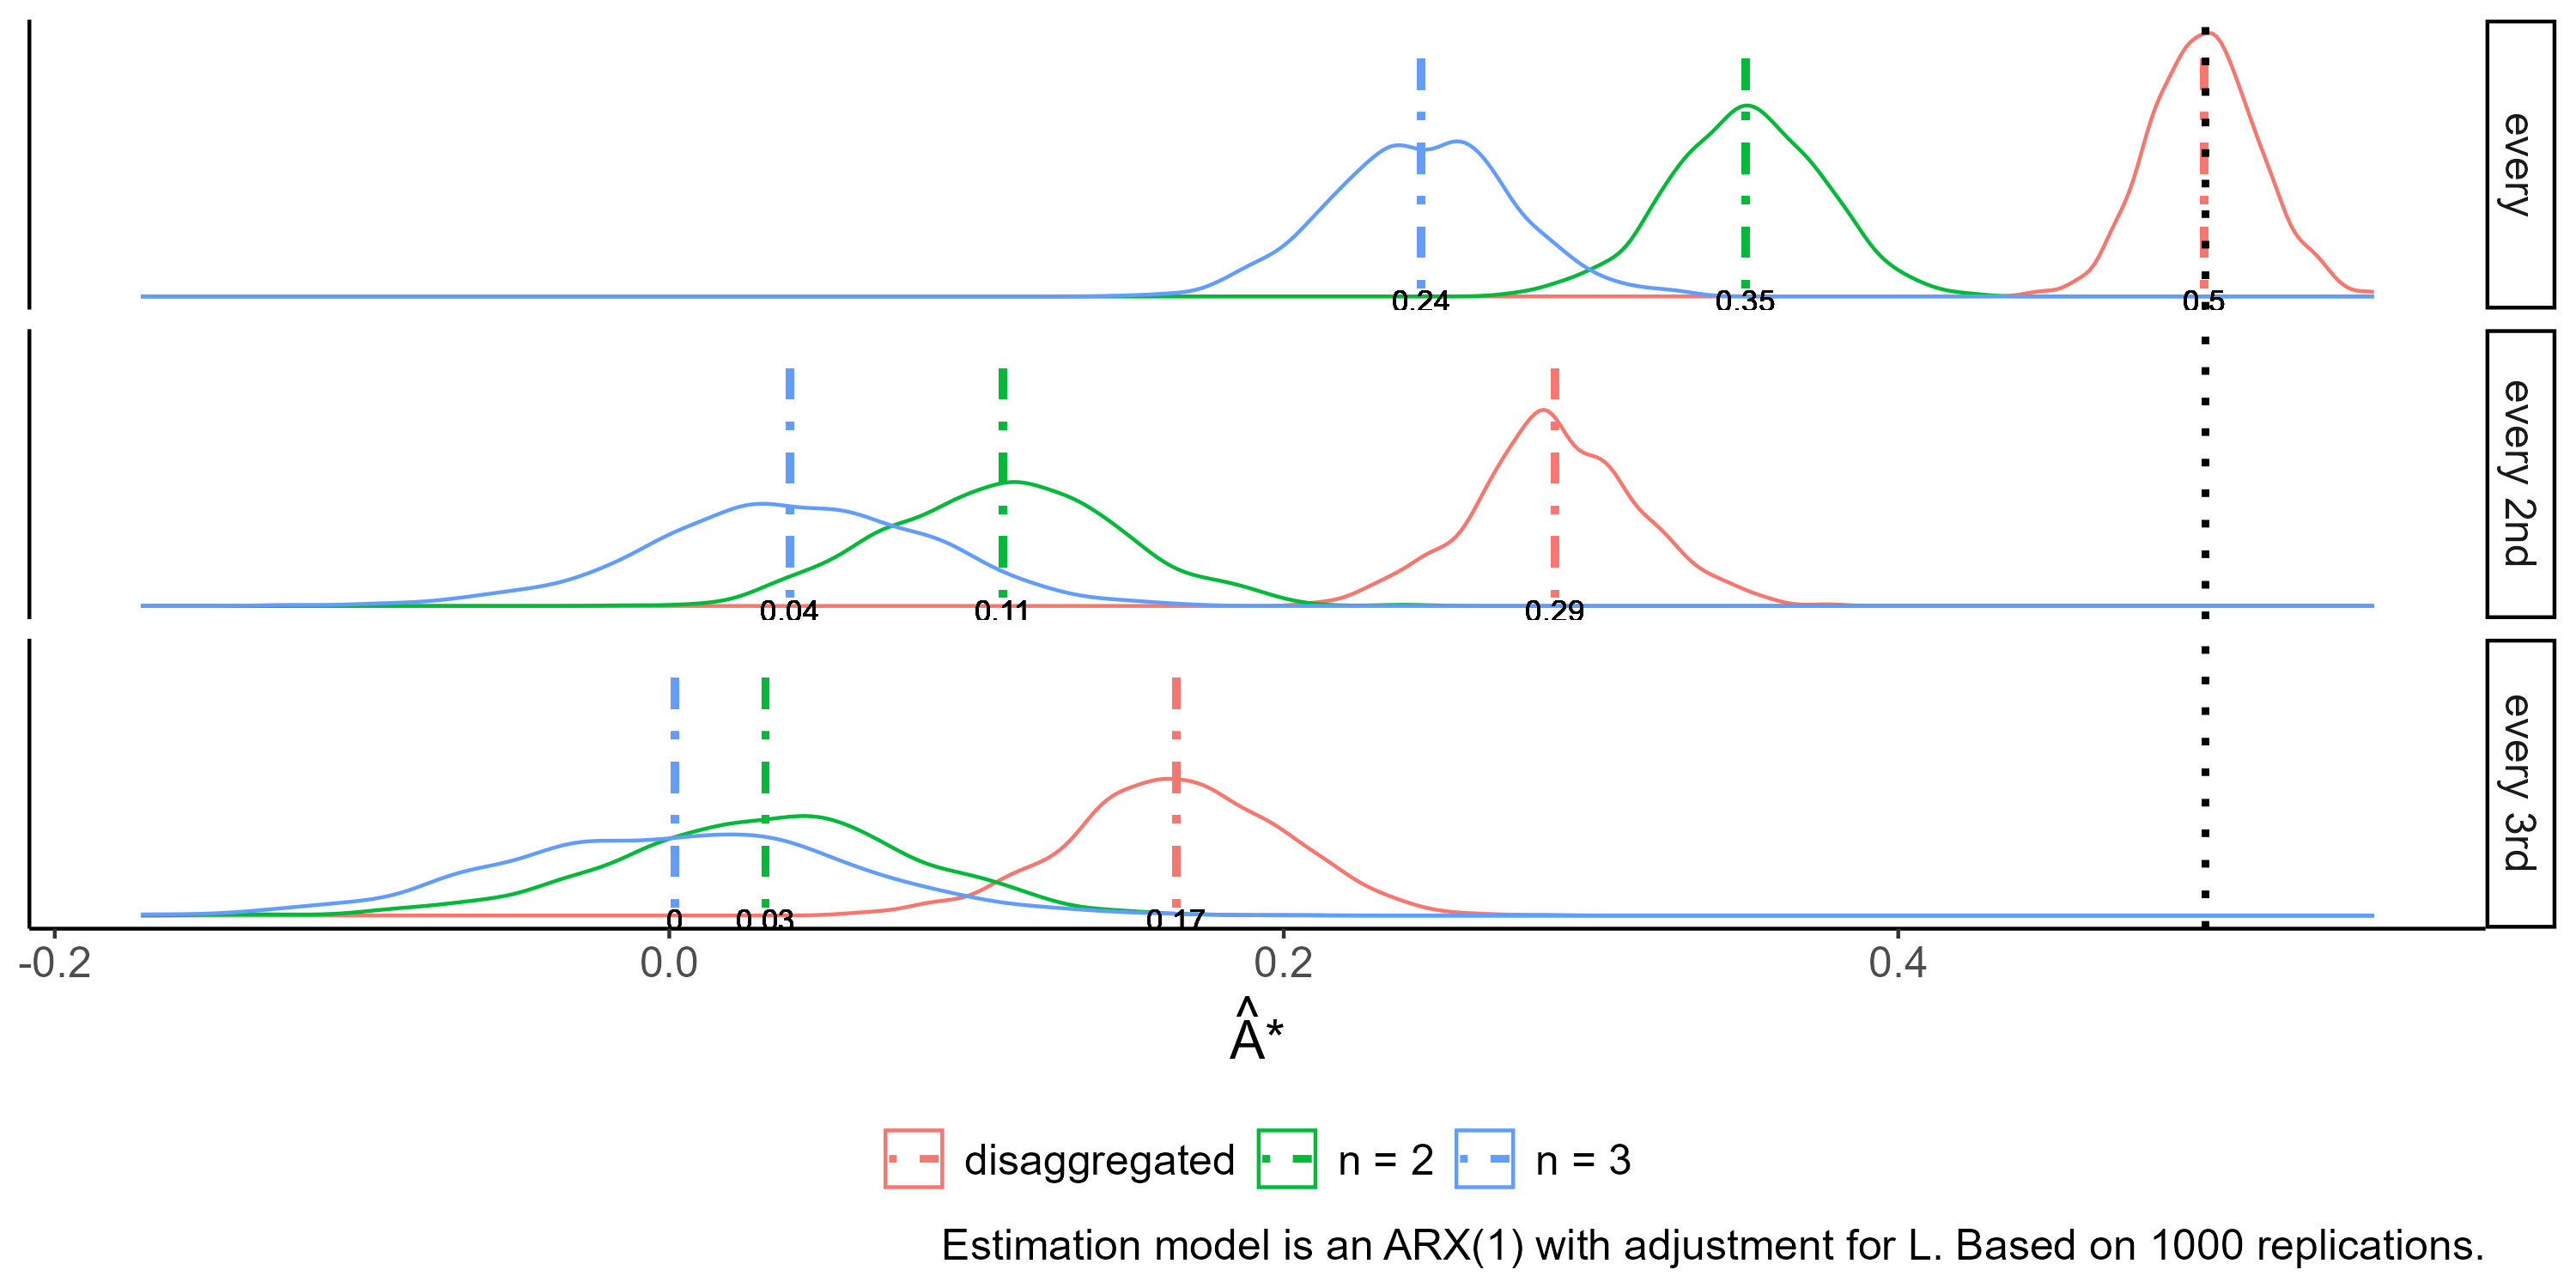
\includegraphics[width=1\linewidth]{figures/plot_AEstimates_VAR1.png}
    \end{figure}    
\end{frame}

%----

\begin{frame}{VAR(1) | Results ARX(1) (adjustment for $L$, sampling distribution $\hat{M}$)}
    \begin{figure}
        \centering
        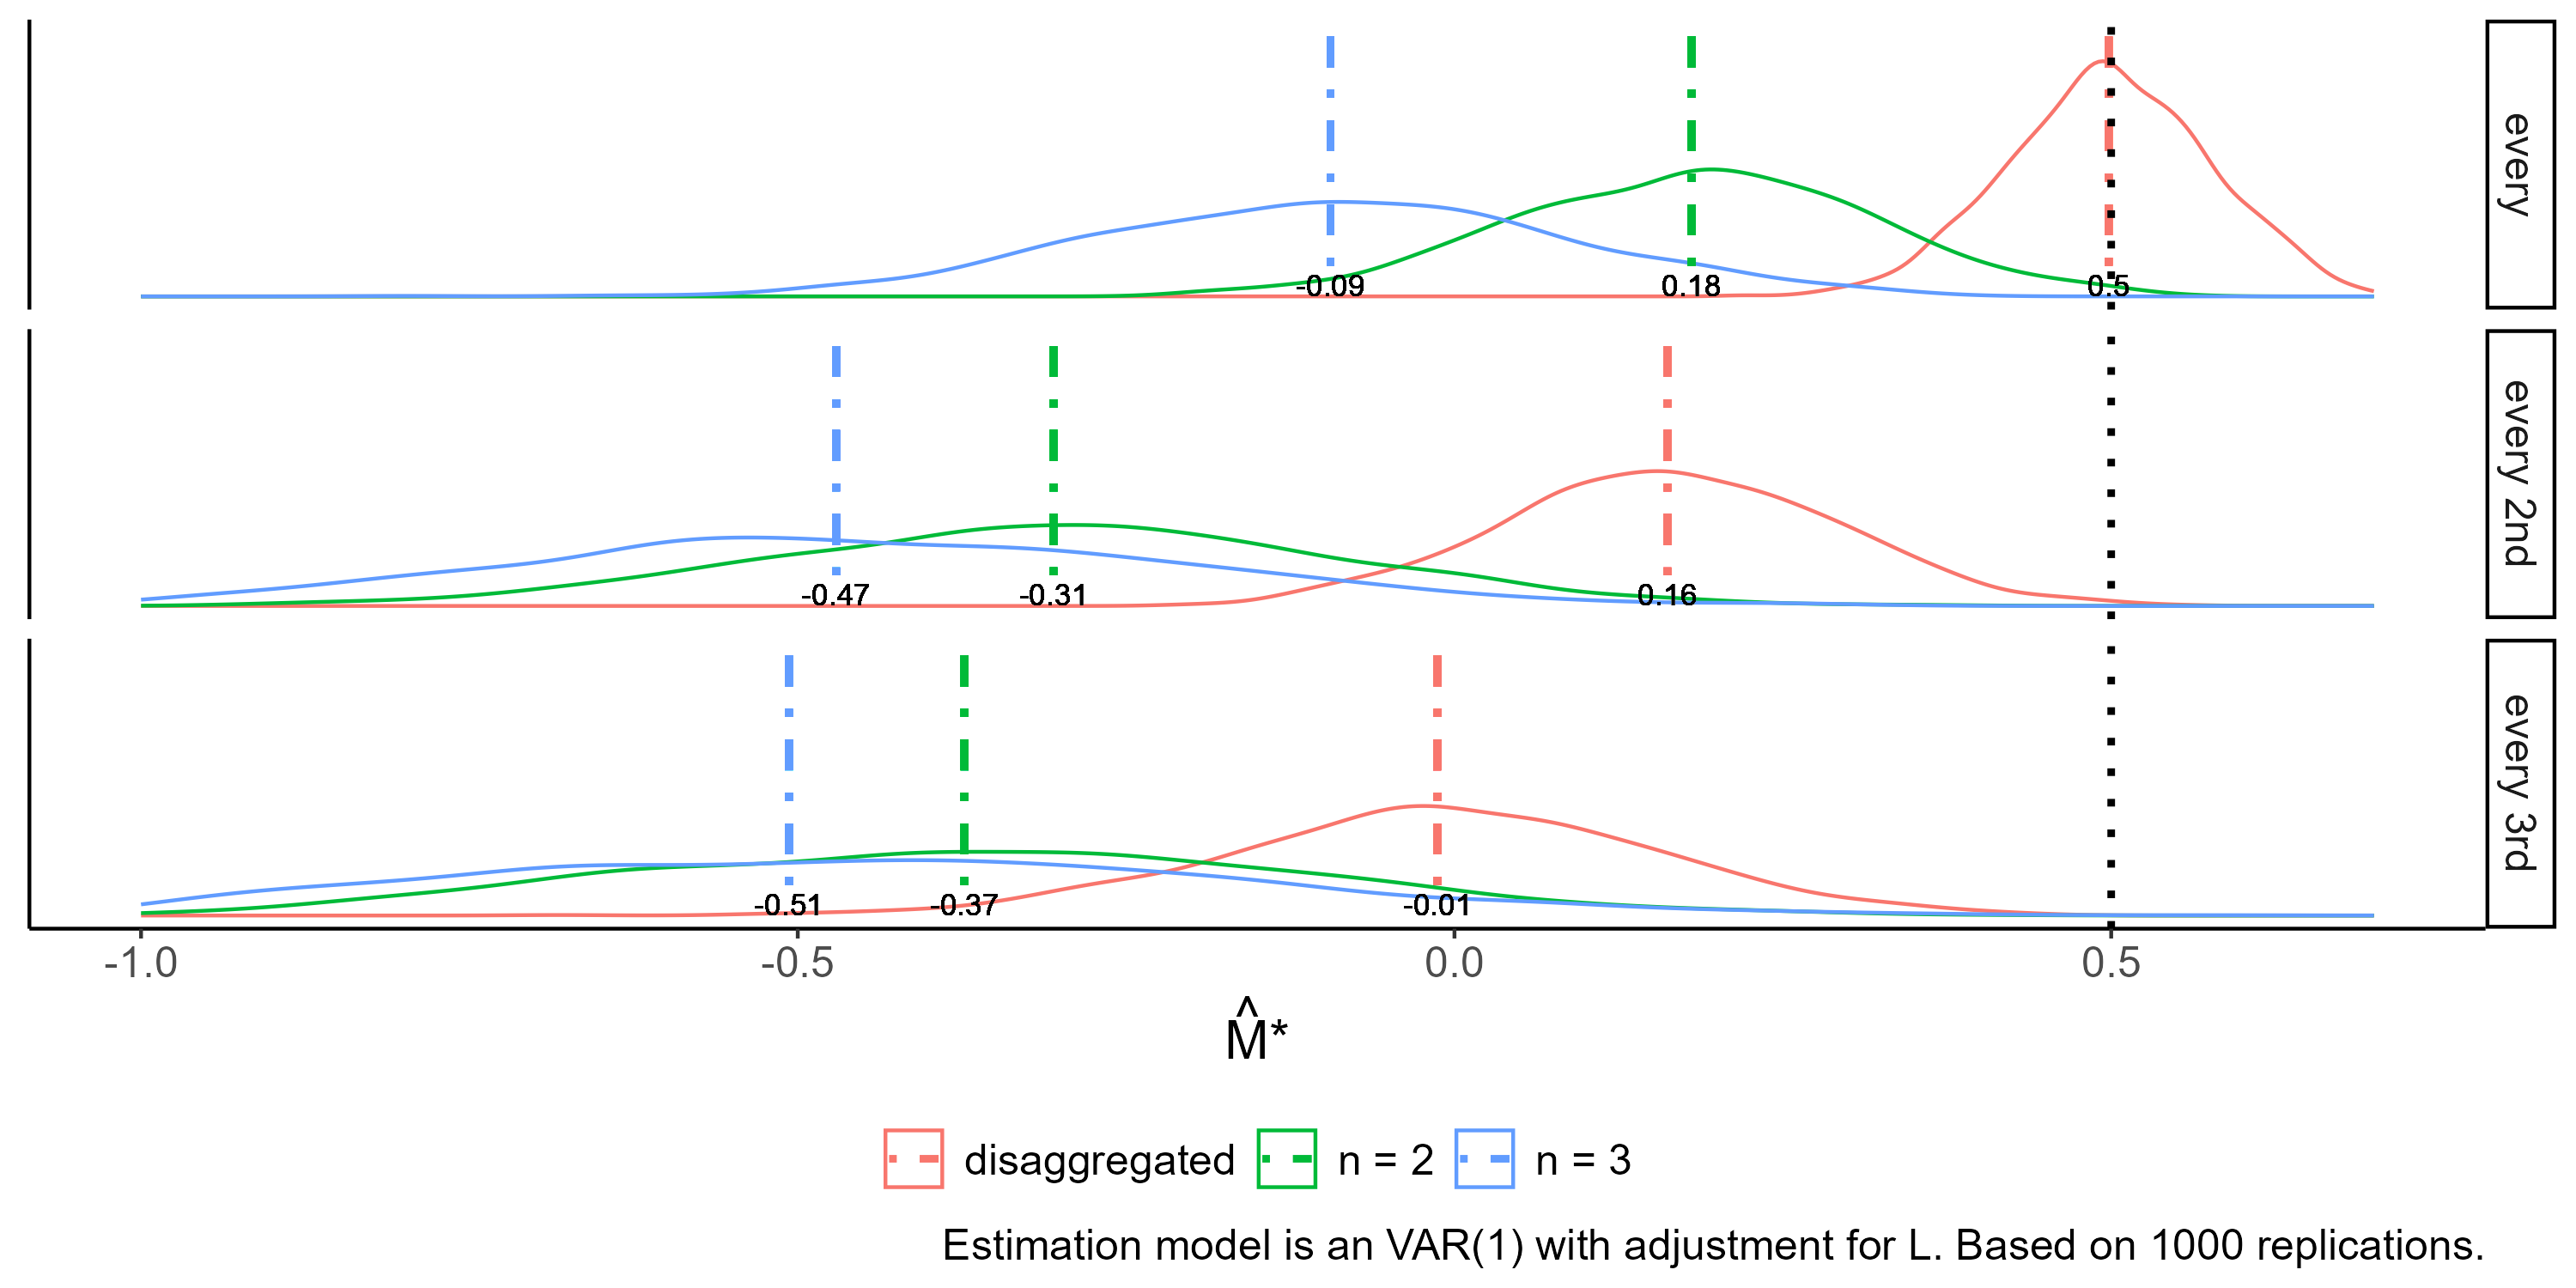
\includegraphics[width=1\linewidth]{figures/plot_MEstimates_VAR1.png}
    \end{figure}    
\end{frame}

%----

\begin{frame}{VAR(1) | Results ARX(1) (sampling distribution $\hat{\beta}_{YL}$)}
    \begin{figure}
        \centering
        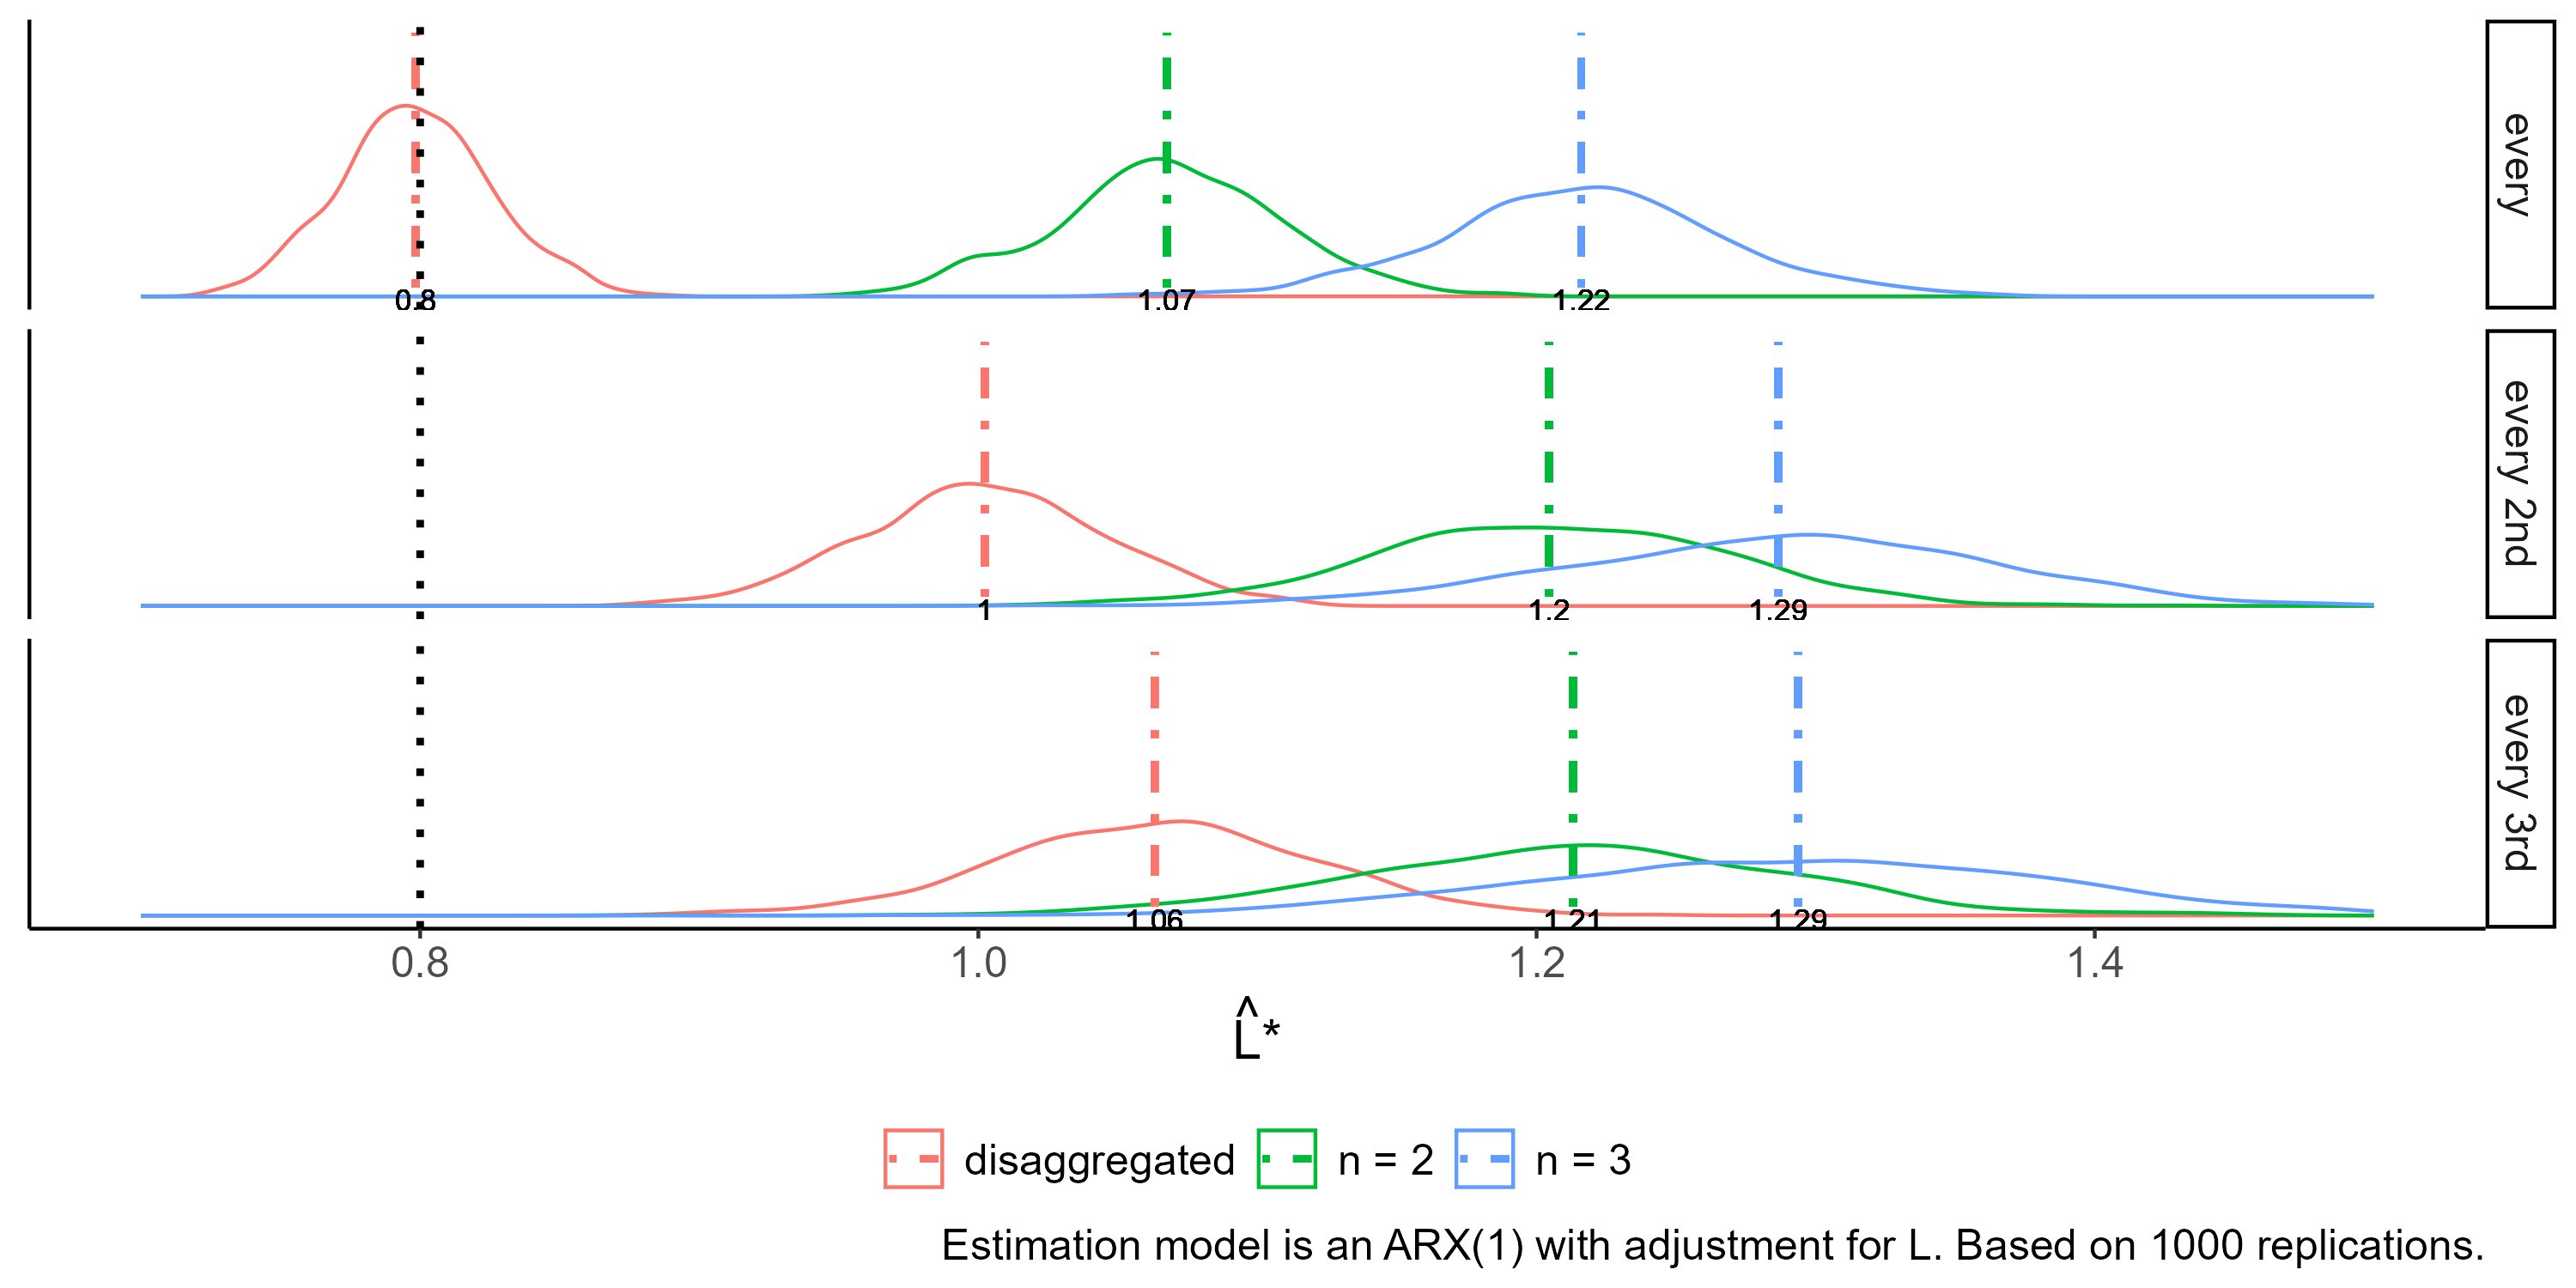
\includegraphics[width=1\linewidth]{figures/plot_hats_betaYL_VAR1.png}
    \end{figure}
\end{frame}

%-----------------------------
\section{Multiple Subjects}
%-----------------------------

%------------------------
\subsection{ML-ARX(1)}
%------------------------

\begin{frame}{ML-ARX(1) | Data generation}
    \textcolor{gray}{
        \textbf{Exposure $X$:} \\
        Exogenous CT Markov Chain with transition probabilities $q_{01} = 0.3$ and $q_{10} = 0.3$.\\
        \bigskip
        \textbf{Outcome $Y$:} \\
        Continuous outcome generated as:
        \begin{equation}
            y_{it} = a y_{i, t-1} + m x_{it} + u_{it}
        \end{equation}
        where $u \sim \mathcal{N}(0,\,\sigma^{2})$, and no random effects. \\
        \bigskip
        \textbf{Aggregation- and missingness-scheme:}\\
        Taking the mean over $n$ periods, where $n \in \{2, 3\}$, and ensure proper aggregates. Analysis with every, every 2nd, or every 3rd observation. \\
    }
    \bigskip
    \textbf{Simulation factors:}\\
    Sample size set to 100, with 120 disaggregated time points per unit. 
\end{frame}

%----

\begin{frame}{ML-ARX(1) | Estimation ML-ARX(1)}
    A multilevel time series model with only random intercept, estimated in Mplus (8.11):\\
    \bigskip
    \begin{table}
        \setlength\extrarowheight{2pt}
        \begin{center}
            \scalebox{0.7}{
                \begin{tabular}{ p{2.8cm} p{9.8cm} }
                \hline
                \\[-2.3mm]
                    \textcolor{blue}{ANALYSIS:} & TYPE = TWOLEVEL;\\
                                                & ESTIMATOR = BAYES;\\
                                                & BITERATION = (2000);
                                                & \\
                    \textcolor{blue}{MODEL:}    & \%WITHIN\%\\
                                                & y ON 0.5*y\&1 0.5*chi;\\
                                                & \\
                                                & \%BETWEEN\% \\
                                                & y;\\
                \\[-2.3mm]
                \hline
                \end{tabular}
            }
        \end{center}
    \end{table}
\end{frame}

%----

\begin{frame}{ML-ARX(1) | $\hat{A}$s from ML-ARX(1) by missingness}
    \begin{figure}
        \centering
        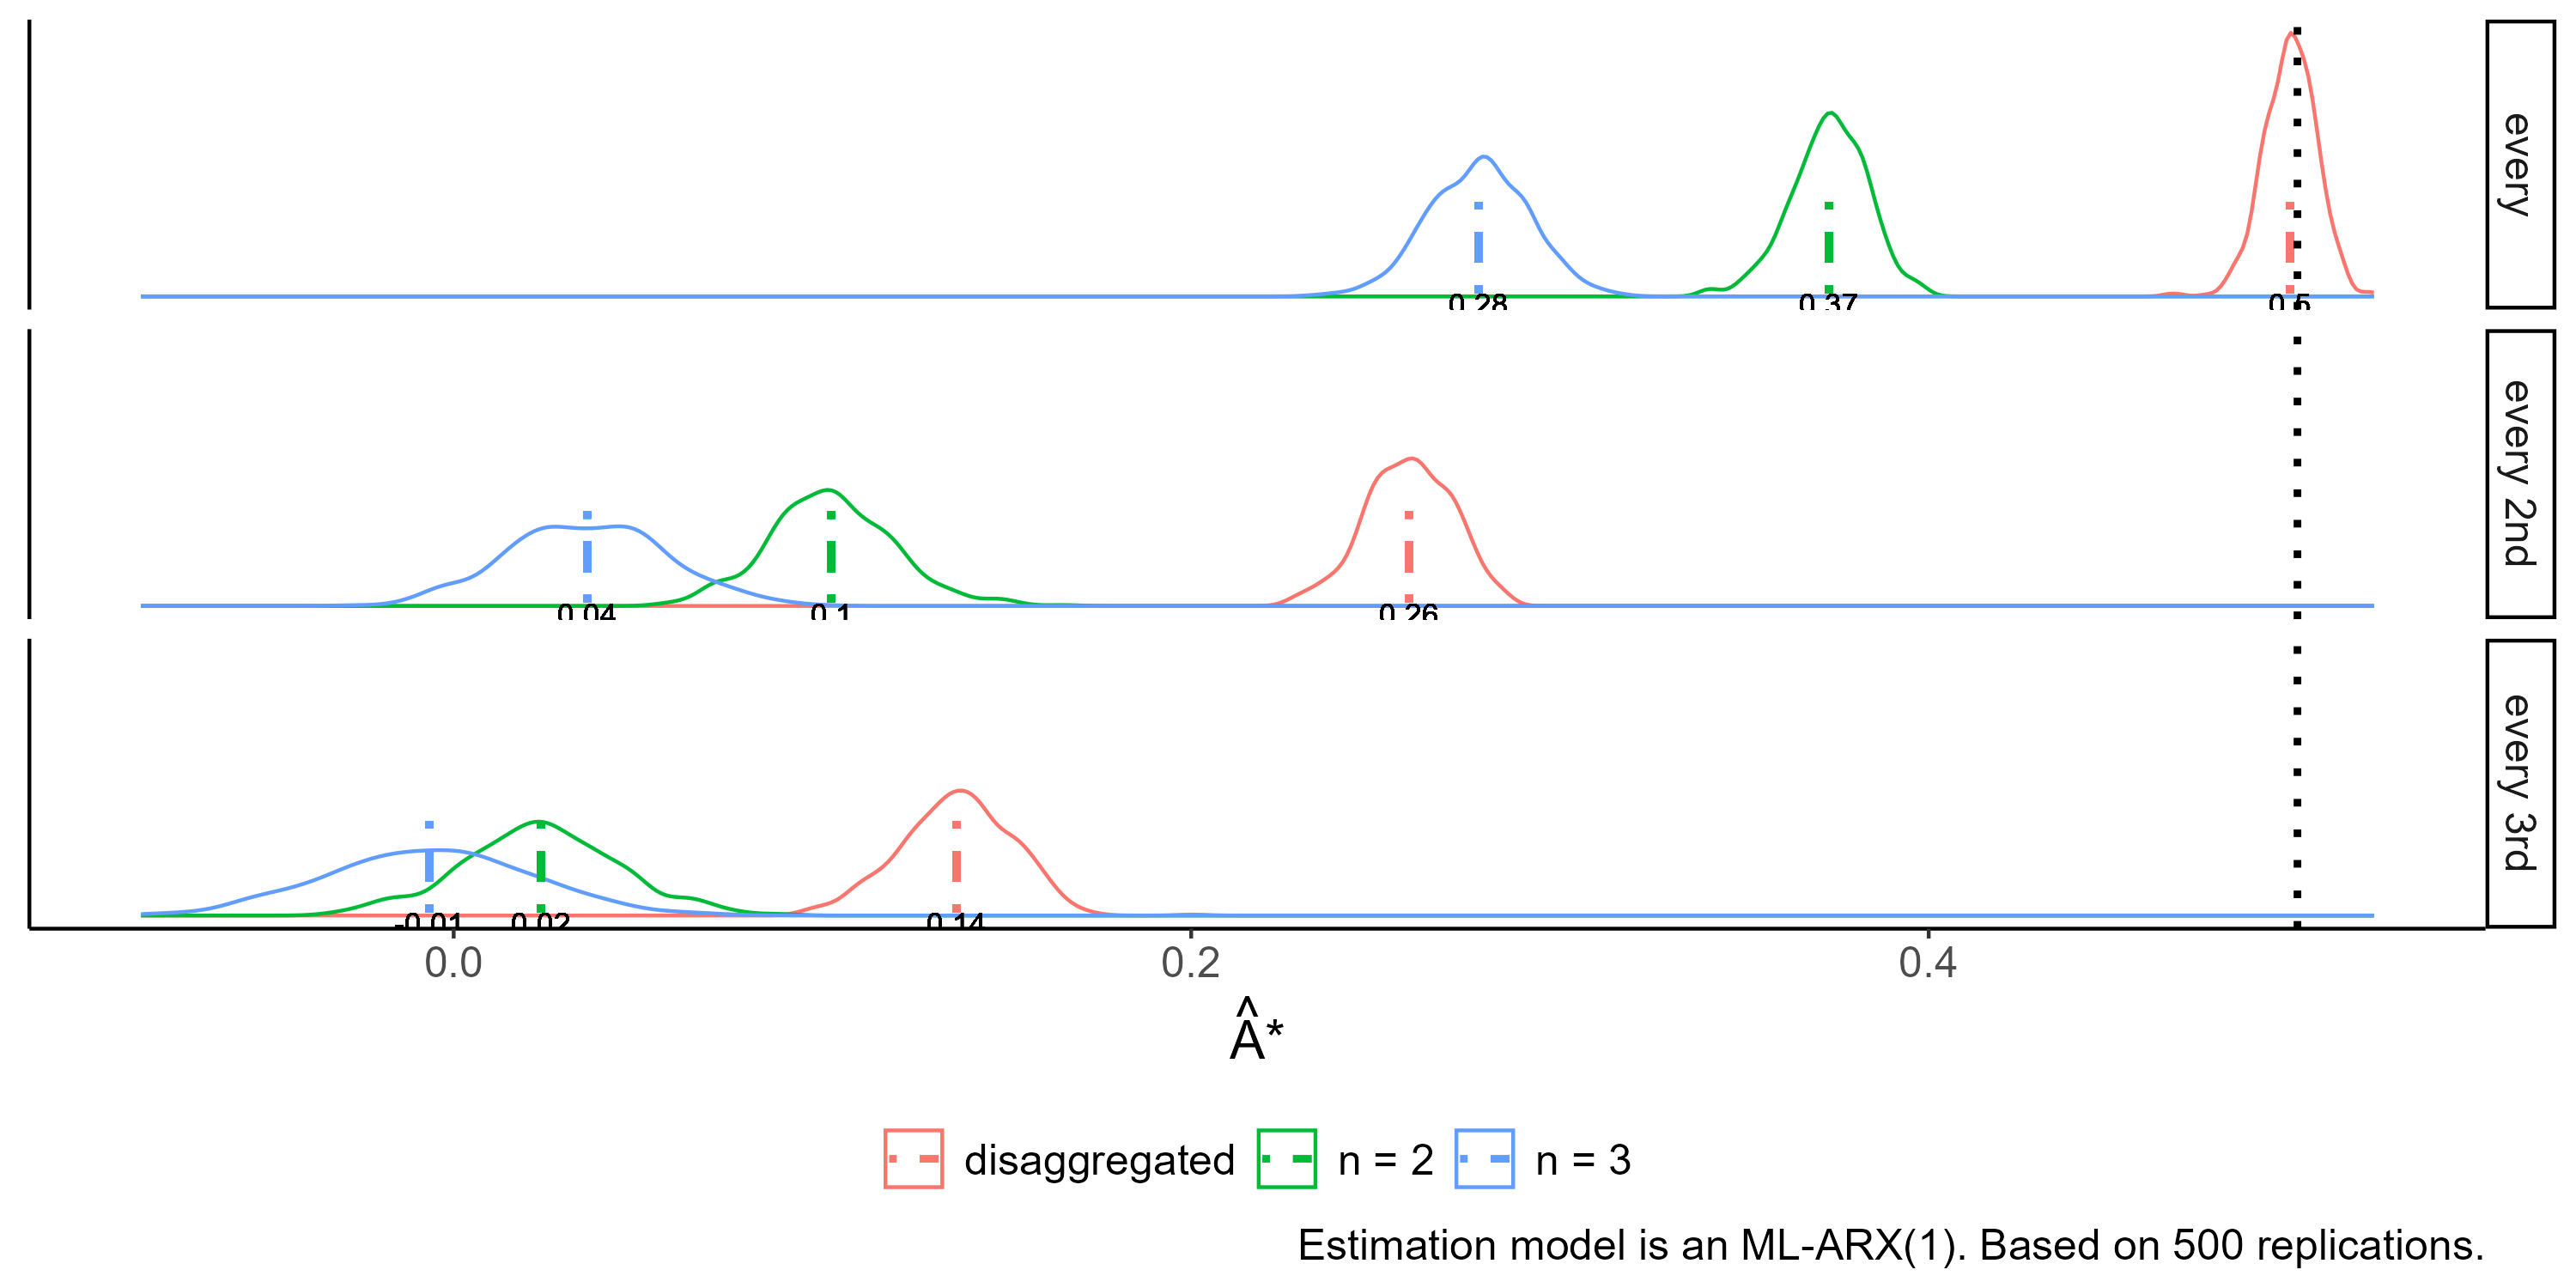
\includegraphics[width=1\linewidth]{figures/plot_AEstimates_MLARX1_missing.png}
    \end{figure}
\end{frame}

%----

\begin{frame}{ML-ARX(1) | $\hat{M}$s from ML-ARX(1) by missingness}
    \begin{figure}
        \centering
        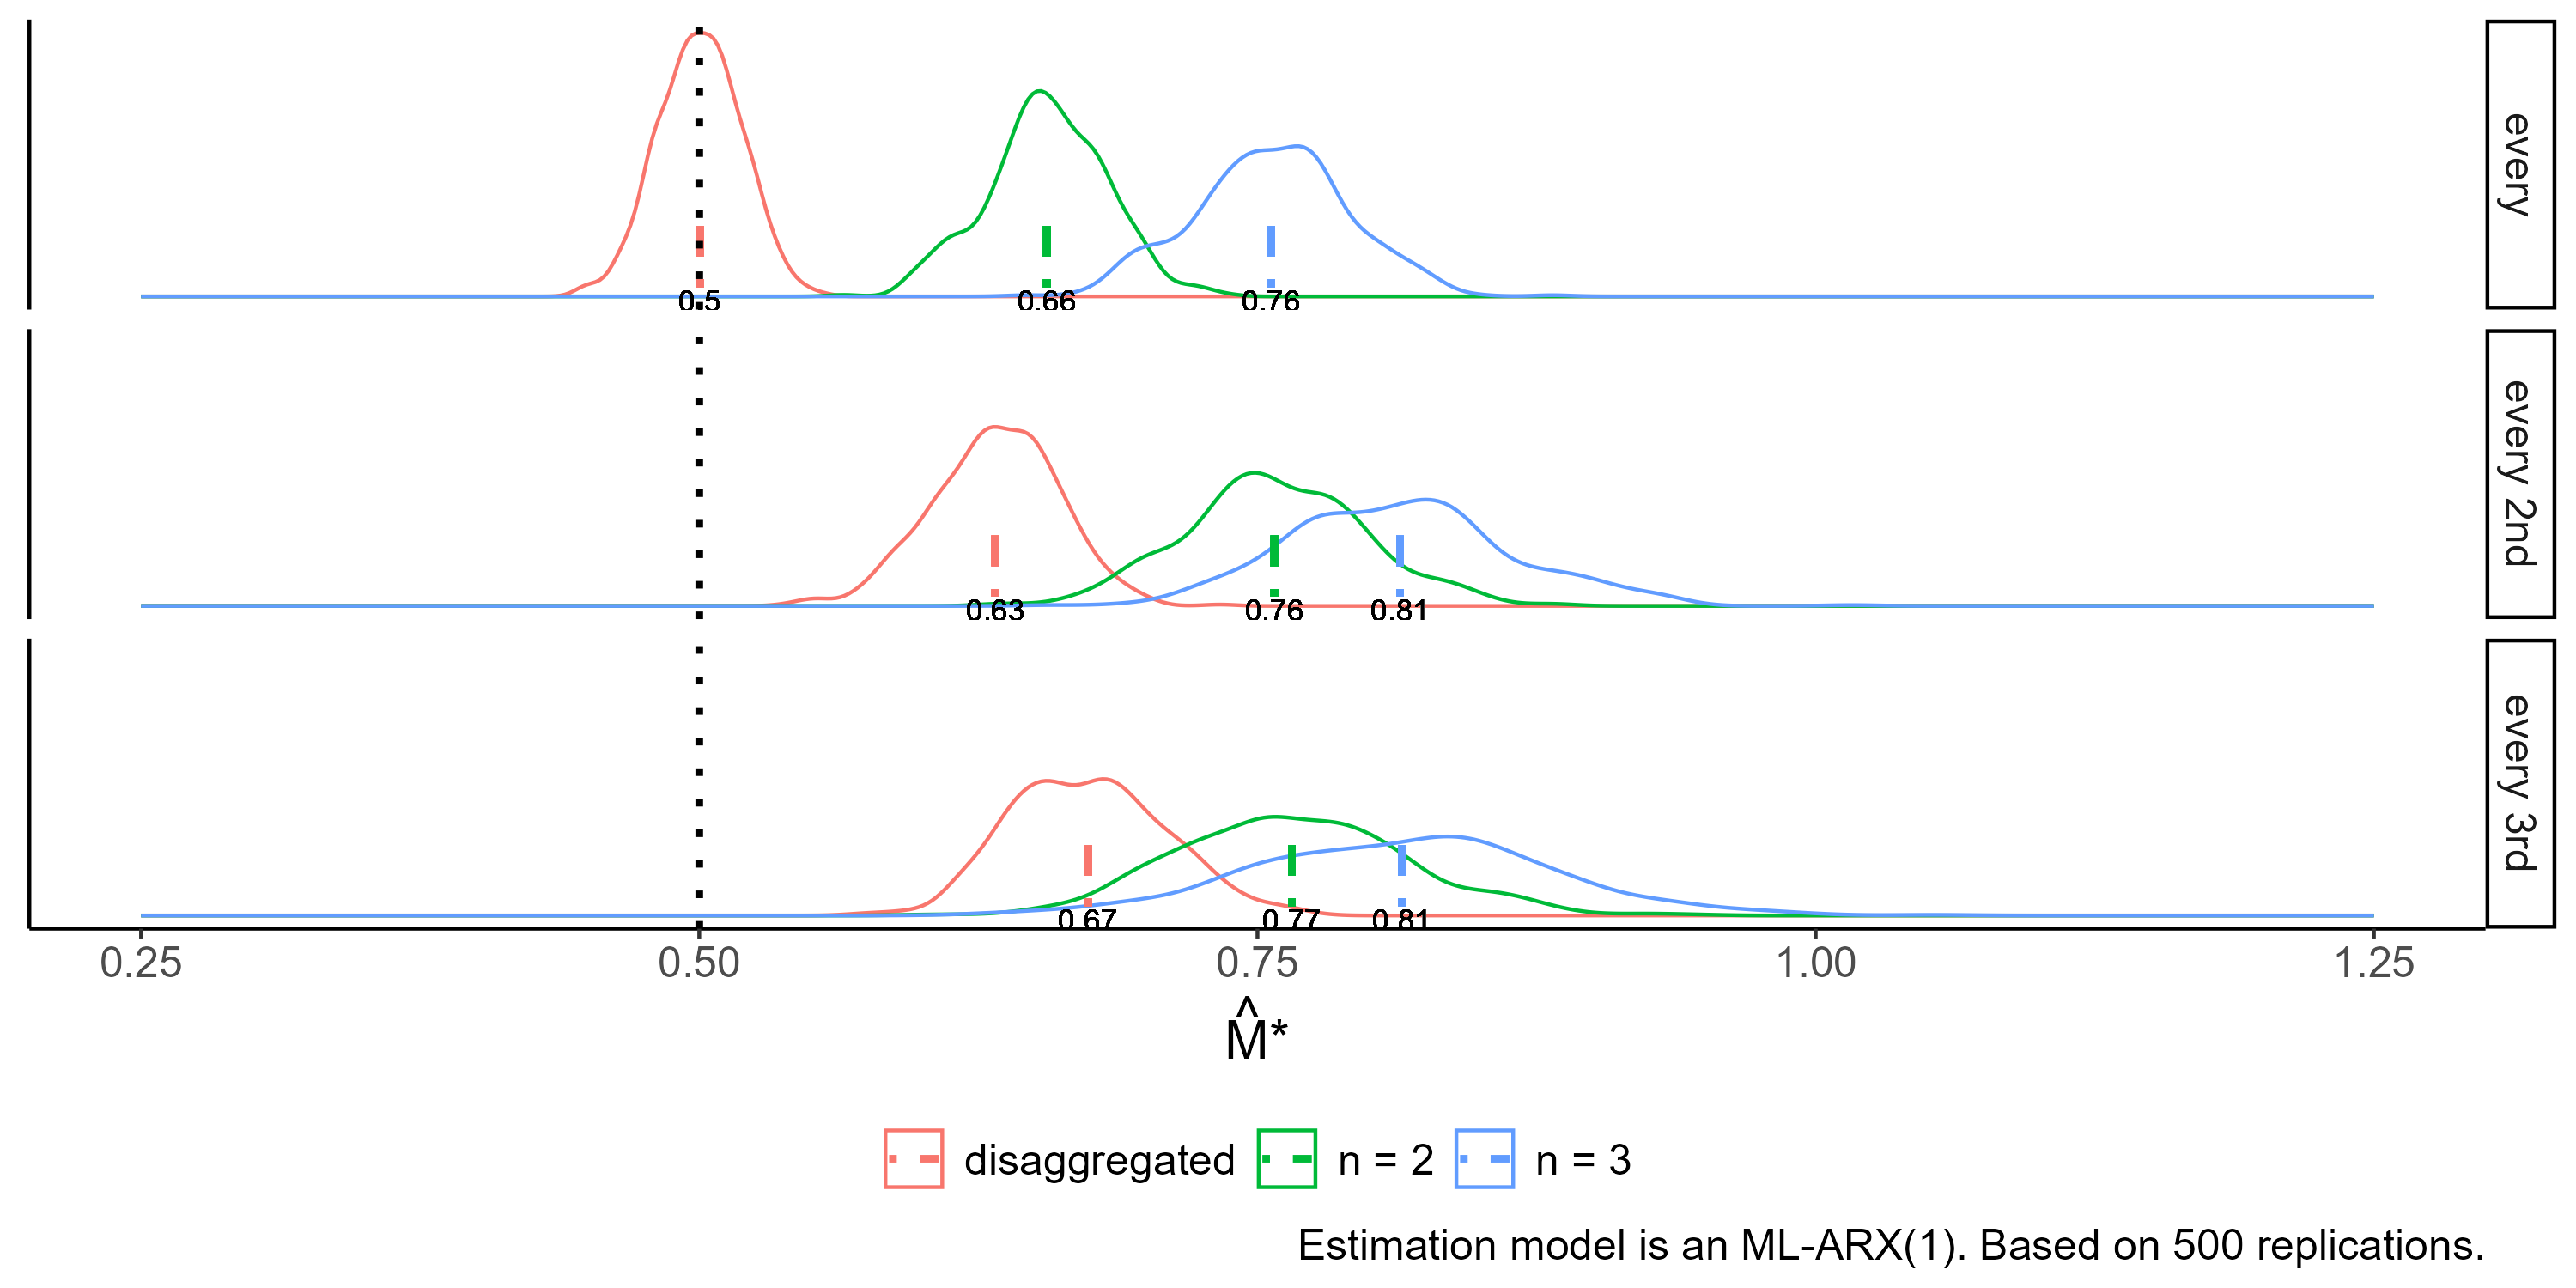
\includegraphics[width=1\linewidth]{figures/plot_MEstimates_MLARX1_missing.png}
    \end{figure}
\end{frame}

%---------------------------------------------------------------------------
\subsection{Including Covariates (Panel-Like Time-Aggregation and Time-Lag)}
%---------------------------------------------------------------------------

\begin{frame}{Data visualization (weekly aggregates, 15 monthly observations)}
    \begin{figure}
        \centering
        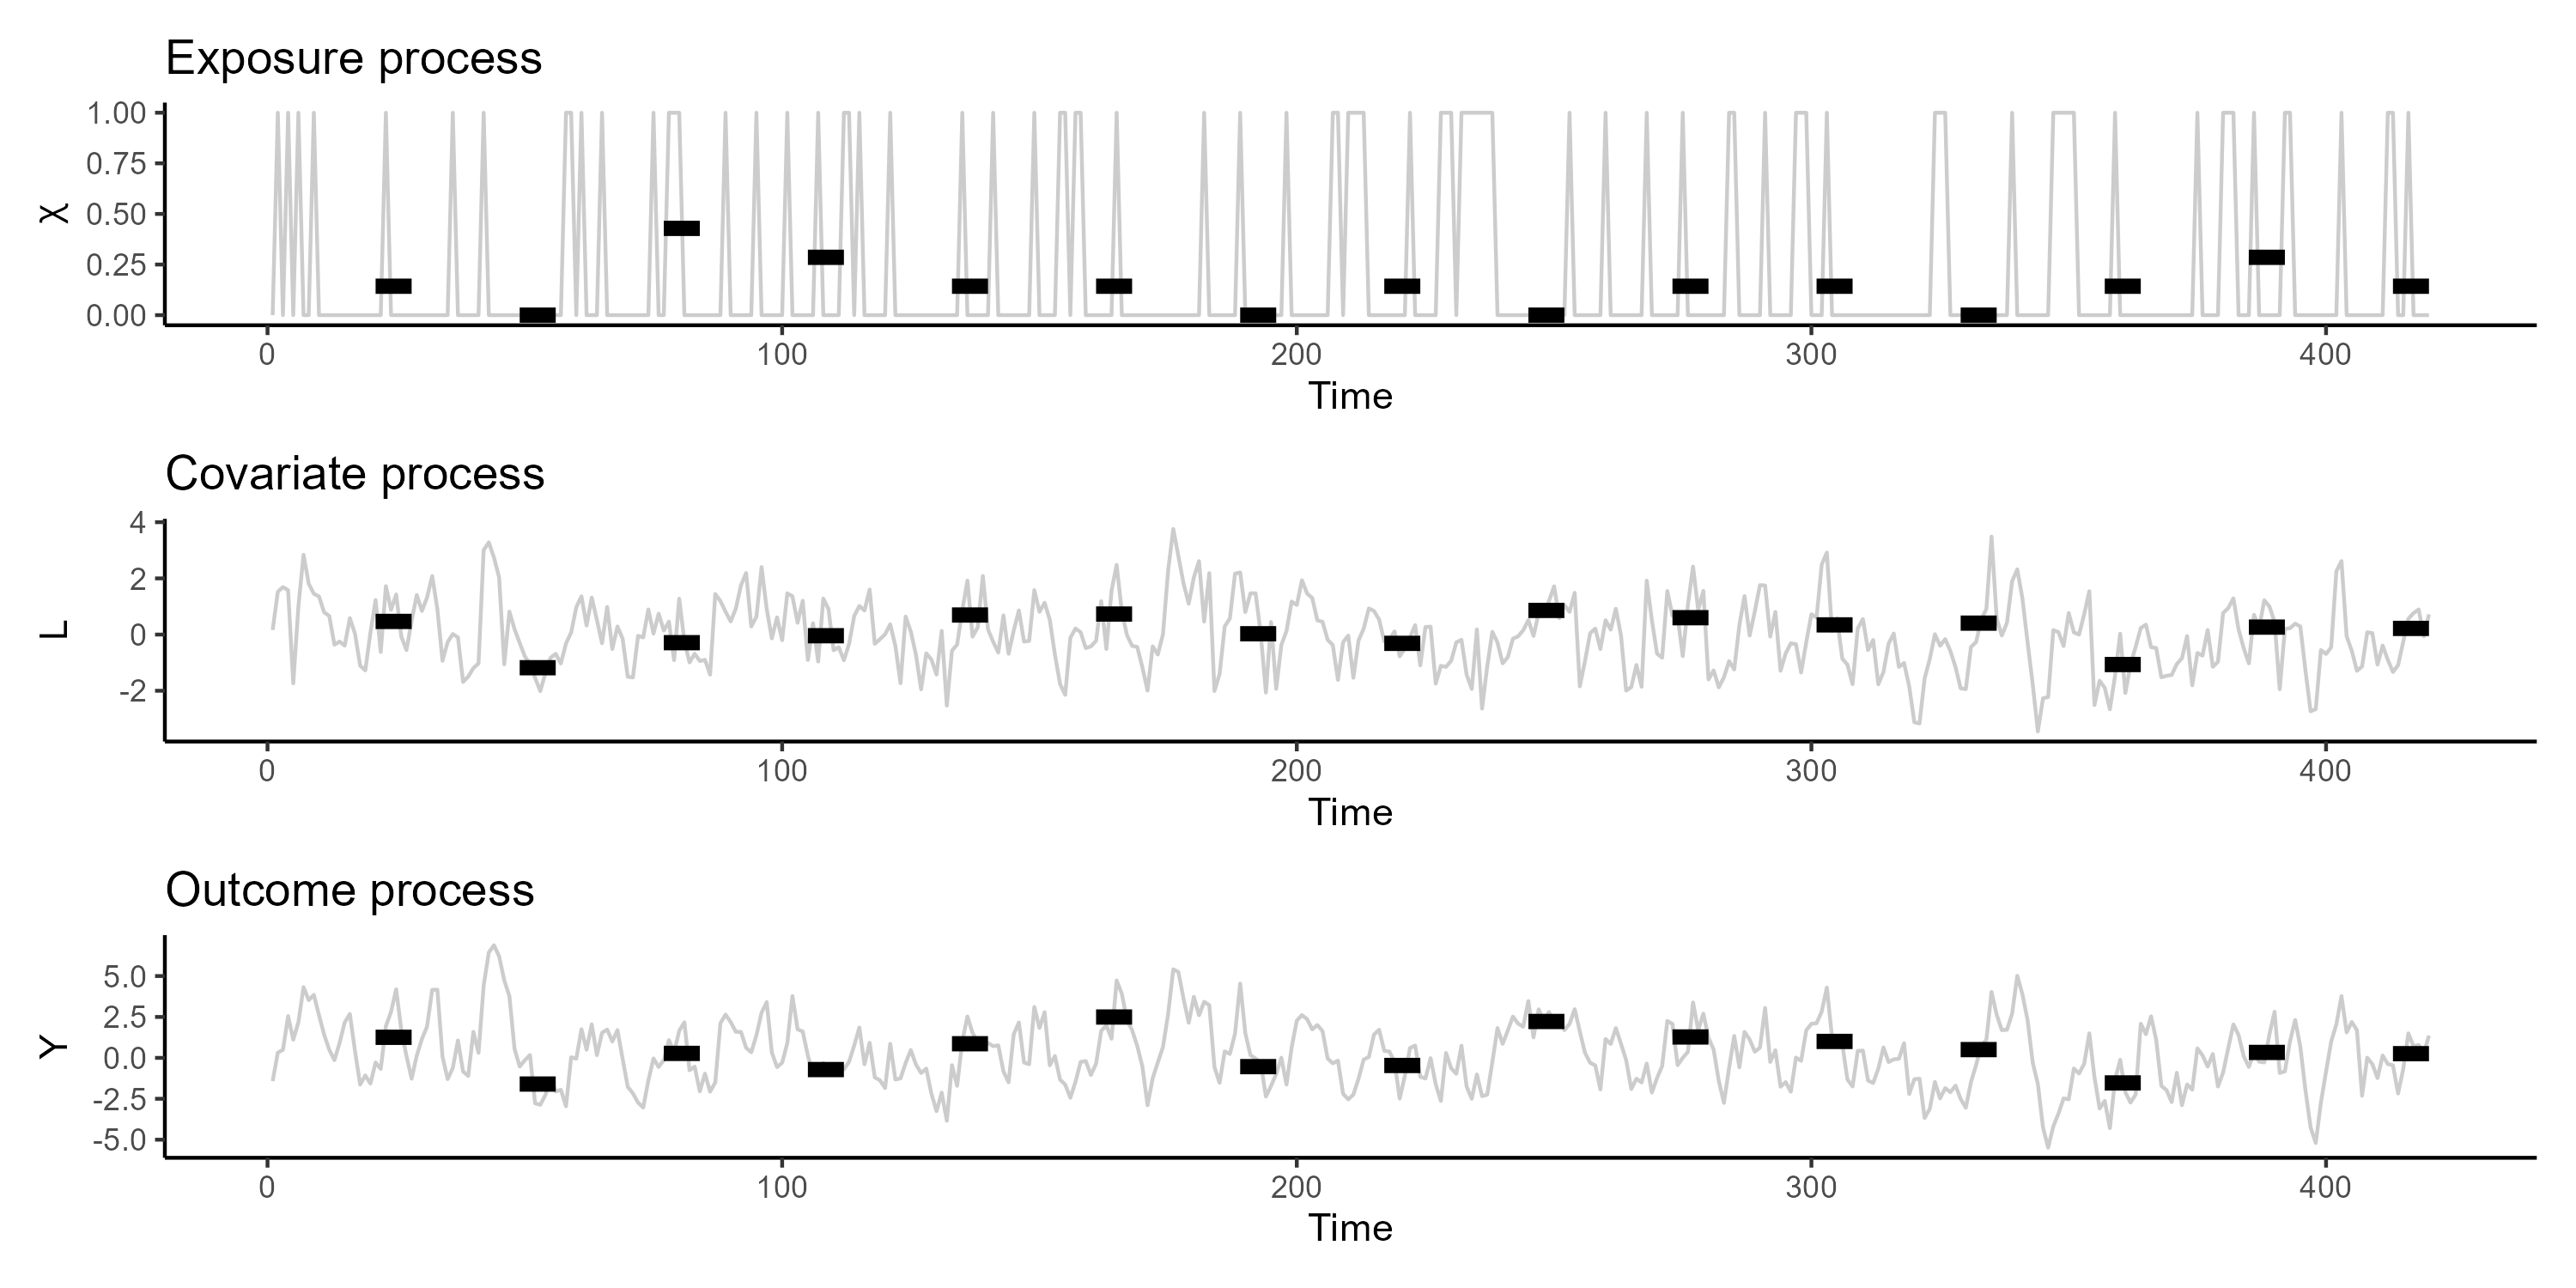
\includegraphics[width=1\linewidth]{figures/plot_dat_MLVAR1_panel.png}
    \end{figure}
\end{frame}

%----

\begin{frame}{ML-ARX(1) | Panel data (weekly aggregates, 15 monthly observations)}
    Estimation model is univariate multilevel DSEM model, in which $Y_{t}$ is regressed on $\chi_{t}$, $\chi_{t - 1}$, $L_{t}$, $L_{t - 1}$, and $Y_{t - 1}$. 
    \begin{table}[]
        \centering
        \begin{tabular}[t]{ccccc}
            \toprule
            Parameter & Population value & Avg & Bias & MCSE \\
            \midrule
            $A$ & 0.5 & -0.011 & -0.511 & 0.001\\
            $M$ & 0.5 & -0.540 & -1.040 & 0.003\\
            beta\_Y\_L & 0.8 & 1.420 & 0.623 & 0.001\\
            beta\_Y\_Lag1L & 0 & 0.022 & 0.022 & 0.001\\
            beta\_Y\_Lag1Chi & 0 & -0.018 & -0.018 & 0.003\\
            \bottomrule
        \end{tabular}
        \caption{\footnotesize{Average estimate (Avg), bias, and Monte Carlo standard errors (MCSE) of the bias for regression coefficients. Based on 1000 replications.}}
    \end{table}
\end{frame}

%----------------------
\subsection{Panel Data}
%----------------------

\begin{frame}{ML-ARX(1) | Panel data generation and estimation}
    \textbf{Data generation:}\\
    Simulated data have a sample size of 500 and 5 repeated measures.\\
    \bigskip
    \textbf{Estimation:}\\
    Overall, we regress $Y_{t}$ on $\chi_{t}$ while adjusting for $\chi_{t - 1}$, $L_{t}$, $L_{t - 1}$, and $Y_{t - 1}$. \\
    \bigskip
    Due to limited number of repeated measures, we switch to models for the analysis of longitudinal data in wide-format:
    \begin{enumerate}
        \item Unidirectional (RI-)CLPM, with both lag-0 and lag-1 relationships. 
        \item Inverse Probability Weighted (IPW) estimation of Marginal Structural Model. 
        \item G-estimation of Structural Nested Mean Model. 
    \end{enumerate}
\end{frame}

%----
    
\begin{frame}{ML-ARX(1) | Estimation using unidirectional (RI-)CLPM}
    \begin{table}[]
        \centering
        \begin{tabular}[t]{ccccc}
            \toprule
            Parameter & Population value & Avg & Bias & MCSE \\
            \midrule
            $A$ & 0.5 & -0.001 & -0.501 & 0.001 \\
            $M$ & 0.5 & -0.538 & -1.040 & 0.005\\
            beta\_Y\_L & 0.8 & 1.420 & 0.619 & 0.001\\
            beta\_Y\_Lag1L & 0 & 0.002 & 0.002 & 0.002\\
            beta\_Y\_Lag1Chi & 0 & -0.004 & -0.004 & 0.006\\
            \bottomrule
        \end{tabular}
        \caption{\footnotesize{Average estimate (Avg), bias, and Monte Carlo standard errors (MCSE) of the bias for regression coefficients. Based on 1000 replications.}}
    \end{table}
\end{frame}


%-------------------
\section{Discussion}
%-------------------

\begin{frame}{Solutions | \textcite{zhang_causal_2011} I}
    \textcite{zhang_causal_2011} focus on continuous time processes, where confounders have been measured only in discrete time. \\
    \bigskip
    They make use of the weak ignorability assumption, $\chi \perp\!\!\!\!\perp Y^{0}$, to identify the ATT. For a Markovian (lag-1) system, conditioning on $Y^{0}_{t_{2}}$ makes $Y^{0}_{t_{3+}}$ and later independent from treatment $\chi_{t_{1}}$. \\
    \bigskip
    \begin{quote}
        ``While both height [outcome] and weight [confounder] reflect the nutritional status of a child, malnutrition usually affects weight more quickly than height, that is, the weight contains leading information for the natural height of the child.''
    \end{quote}
    \bigskip
    \begin{quote}
        ``The idea behind the controlling-the-future method is to condition on a "surrogate" for $L_{1/2}$.''
    \end{quote}
\end{frame}

%----

\begin{frame}{Solutions | \textcite{zhang_causal_2011} II}
    \begin{figure}
        \centering
        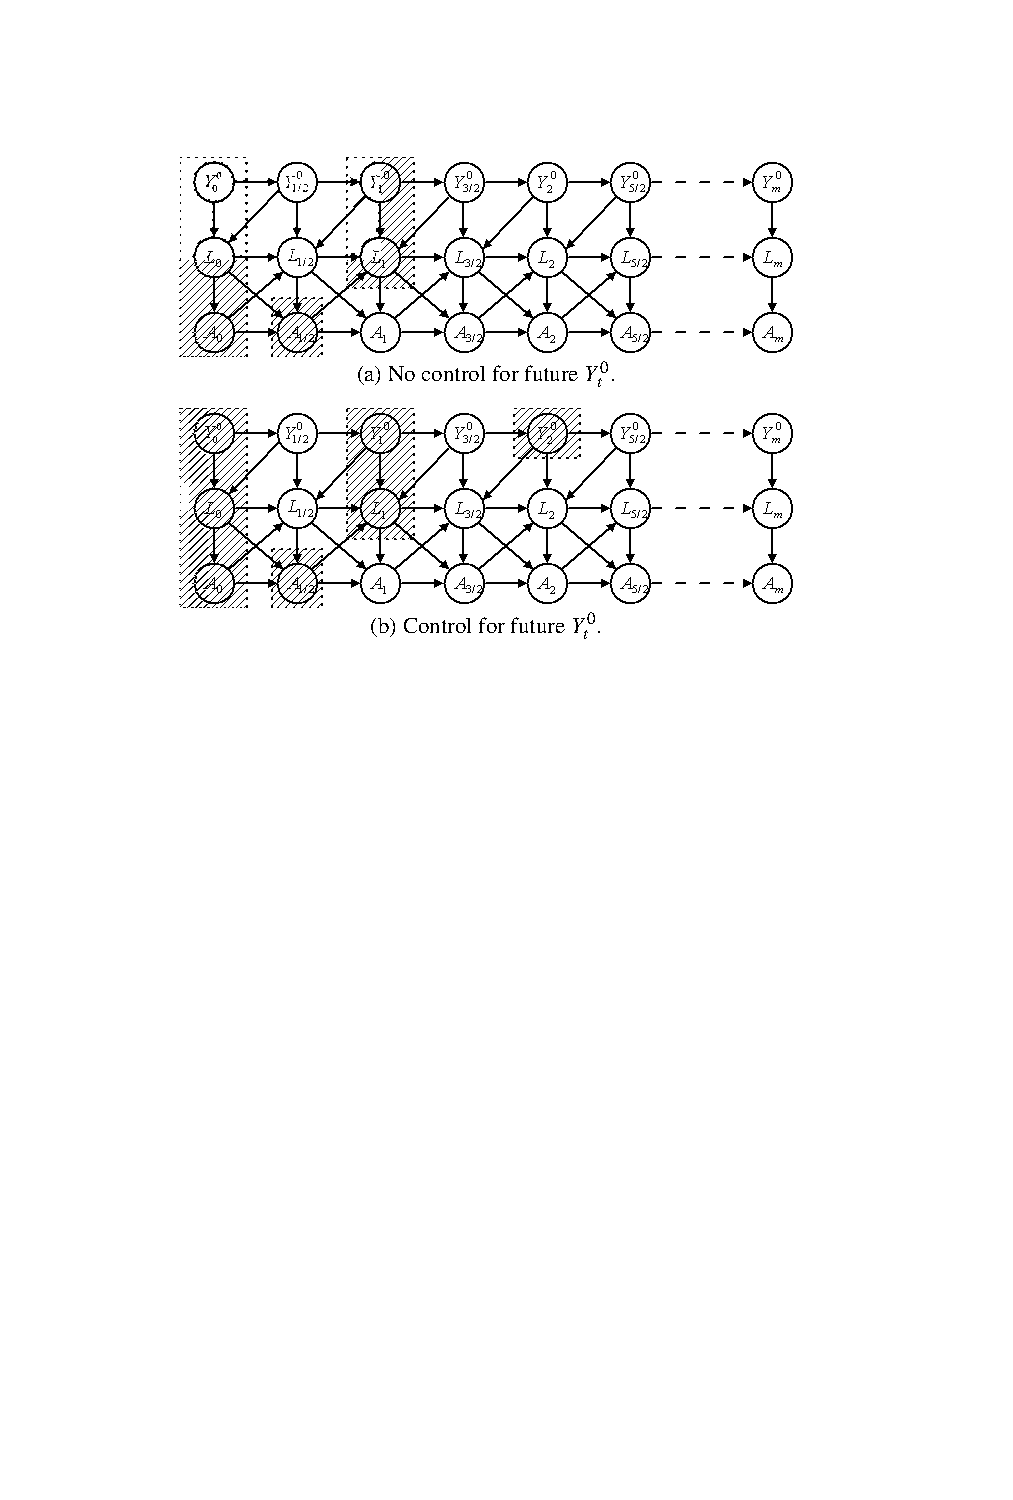
\includegraphics[width=0.65\linewidth]{figures/DAG_leadingLt.pdf}
    \end{figure}
\end{frame}

%----

\begin{frame}{Solutions | Continuous time modeling}
    When we observe individuals at random measurement occasions across time, we might have the required information for identification. 
\end{frame}

%----

\begin{frame}{Notation}
    \begin{table}[]
        \centering
        \footnotesize
        \begin{tabular}{p{2cm}p{11cm}}
            $t$ & time \\
            $m$ & number of time periods to aggregate over\\
            $k$ & measurement occasion \\
            & \\
            $X_{k_{m}}, Y_{k_{m}}, L_{k_{m}}$ & exposure, outcome, and covariate(s) aggregated over $m$ periods, where $k = \ceil{\frac{t}{m}}$\\
                & \\
            $\epsilon_{k_{m}}$ & residual in model for aggregated process\\
            & \\
            $\phi_{k_{m}}$ & autoregressive effect of outcome in aggregated process\\
            & \\
            $\beta_{Y_{k_{m}}X_{k_{m} - 1}}$ & cross(-lagged) effect exposure to outcome in aggregated process\\
        \end{tabular}
    \end{table}
\end{frame}

%----

\begin{frame}{Literature to be explored}
    
\end{frame}

%----

\begin{frame}{Take-aways}
    \begin{itemize}
        \item Yet another reminder to incorporate time explicitly in your causal estimand, rather than posthoc time-aggregation? 
        
    \end{itemize}
\end{frame}

%----

\begin{frame}[allowframebreaks, noframenumbering]{References}
    \printbibliography
\end{frame}
    
\end{document}
